\documentclass[]{DissertateUSU}
\usepackage{lmodern}
\usepackage{amssymb,amsmath}
\usepackage{ifxetex,ifluatex}
\usepackage{fixltx2e} % provides \textsubscript
\ifnum 0\ifxetex 1\fi\ifluatex 1\fi=0 % if pdftex
  \usepackage[T1]{fontenc}
  \usepackage[utf8]{inputenc}
\else % if luatex or xelatex
  \ifxetex
    \usepackage{mathspec}
  \else
    \usepackage{fontspec}
  \fi
  \defaultfontfeatures{Ligatures=TeX,Scale=MatchLowercase}
\fi
% use upquote if available, for straight quotes in verbatim environments
\IfFileExists{upquote.sty}{\usepackage{upquote}}{}
% use microtype if available
\IfFileExists{microtype.sty}{%
\usepackage{microtype}
\UseMicrotypeSet[protrusion]{basicmath} % disable protrusion for tt fonts
}{}
\usepackage[top=1in,bottom=1in,right=1in,left=1.5in]{geometry}
\usepackage{hyperref}
\hypersetup{unicode=true,
            pdftitle={Marginal Mediation Analysis: A New Framework for Interpretable Mediated Effects},
            pdfauthor={Tyson S. Barrett},
            pdfborder={0 0 0},
            breaklinks=true}
\urlstyle{same}  % don't use monospace font for urls
\usepackage{color}
\usepackage{fancyvrb}
\newcommand{\VerbBar}{|}
\newcommand{\VERB}{\Verb[commandchars=\\\{\}]}
\DefineVerbatimEnvironment{Highlighting}{Verbatim}{commandchars=\\\{\}}
% Add ',fontsize=\small' for more characters per line
\usepackage{framed}
\definecolor{shadecolor}{RGB}{248,248,248}
\newenvironment{Shaded}{\begin{snugshade}}{\end{snugshade}}
\newcommand{\KeywordTok}[1]{\textcolor[rgb]{0.13,0.29,0.53}{\textbf{#1}}}
\newcommand{\DataTypeTok}[1]{\textcolor[rgb]{0.13,0.29,0.53}{#1}}
\newcommand{\DecValTok}[1]{\textcolor[rgb]{0.00,0.00,0.81}{#1}}
\newcommand{\BaseNTok}[1]{\textcolor[rgb]{0.00,0.00,0.81}{#1}}
\newcommand{\FloatTok}[1]{\textcolor[rgb]{0.00,0.00,0.81}{#1}}
\newcommand{\ConstantTok}[1]{\textcolor[rgb]{0.00,0.00,0.00}{#1}}
\newcommand{\CharTok}[1]{\textcolor[rgb]{0.31,0.60,0.02}{#1}}
\newcommand{\SpecialCharTok}[1]{\textcolor[rgb]{0.00,0.00,0.00}{#1}}
\newcommand{\StringTok}[1]{\textcolor[rgb]{0.31,0.60,0.02}{#1}}
\newcommand{\VerbatimStringTok}[1]{\textcolor[rgb]{0.31,0.60,0.02}{#1}}
\newcommand{\SpecialStringTok}[1]{\textcolor[rgb]{0.31,0.60,0.02}{#1}}
\newcommand{\ImportTok}[1]{#1}
\newcommand{\CommentTok}[1]{\textcolor[rgb]{0.56,0.35,0.01}{\textit{#1}}}
\newcommand{\DocumentationTok}[1]{\textcolor[rgb]{0.56,0.35,0.01}{\textbf{\textit{#1}}}}
\newcommand{\AnnotationTok}[1]{\textcolor[rgb]{0.56,0.35,0.01}{\textbf{\textit{#1}}}}
\newcommand{\CommentVarTok}[1]{\textcolor[rgb]{0.56,0.35,0.01}{\textbf{\textit{#1}}}}
\newcommand{\OtherTok}[1]{\textcolor[rgb]{0.56,0.35,0.01}{#1}}
\newcommand{\FunctionTok}[1]{\textcolor[rgb]{0.00,0.00,0.00}{#1}}
\newcommand{\VariableTok}[1]{\textcolor[rgb]{0.00,0.00,0.00}{#1}}
\newcommand{\ControlFlowTok}[1]{\textcolor[rgb]{0.13,0.29,0.53}{\textbf{#1}}}
\newcommand{\OperatorTok}[1]{\textcolor[rgb]{0.81,0.36,0.00}{\textbf{#1}}}
\newcommand{\BuiltInTok}[1]{#1}
\newcommand{\ExtensionTok}[1]{#1}
\newcommand{\PreprocessorTok}[1]{\textcolor[rgb]{0.56,0.35,0.01}{\textit{#1}}}
\newcommand{\AttributeTok}[1]{\textcolor[rgb]{0.77,0.63,0.00}{#1}}
\newcommand{\RegionMarkerTok}[1]{#1}
\newcommand{\InformationTok}[1]{\textcolor[rgb]{0.56,0.35,0.01}{\textbf{\textit{#1}}}}
\newcommand{\WarningTok}[1]{\textcolor[rgb]{0.56,0.35,0.01}{\textbf{\textit{#1}}}}
\newcommand{\AlertTok}[1]{\textcolor[rgb]{0.94,0.16,0.16}{#1}}
\newcommand{\ErrorTok}[1]{\textcolor[rgb]{0.64,0.00,0.00}{\textbf{#1}}}
\newcommand{\NormalTok}[1]{#1}
\usepackage{graphicx,grffile}
\makeatletter
\def\maxwidth{\ifdim\Gin@nat@width>\linewidth\linewidth\else\Gin@nat@width\fi}
\def\maxheight{\ifdim\Gin@nat@height>\textheight\textheight\else\Gin@nat@height\fi}
\makeatother
% Scale images if necessary, so that they will not overflow the page
% margins by default, and it is still possible to overwrite the defaults
% using explicit options in \includegraphics[width, height, ...]{}
\setkeys{Gin}{width=\maxwidth,height=\maxheight,keepaspectratio}
\IfFileExists{parskip.sty}{%
\usepackage{parskip}
}{% else
\setlength{\parindent}{0pt}
\setlength{\parskip}{6pt plus 2pt minus 1pt}
}
\setlength{\emergencystretch}{3em}  % prevent overfull lines
\providecommand{\tightlist}{%
  \setlength{\itemsep}{0pt}\setlength{\parskip}{0pt}}
\setcounter{secnumdepth}{0}
% Redefines (sub)paragraphs to behave more like sections
\ifx\paragraph\undefined\else
\let\oldparagraph\paragraph
\renewcommand{\paragraph}[1]{\oldparagraph{#1}\mbox{}}
\fi
\ifx\subparagraph\undefined\else
\let\oldsubparagraph\subparagraph
\renewcommand{\subparagraph}[1]{\oldsubparagraph{#1}\mbox{}}
\fi

%%% Use protect on footnotes to avoid problems with footnotes in titles
\let\rmarkdownfootnote\footnote%
\def\footnote{\protect\rmarkdownfootnote}

%%% Change title format to be more compact
\usepackage{titling}

% Create subtitle command for use in maketitle
\newcommand{\subtitle}[1]{
  \posttitle{
    \begin{center}\large#1\end{center}
    }
}

\setlength{\droptitle}{-2em}

  \title{Marginal Mediation Analysis: A New Framework for Interpretable Mediated
Effects}
    \pretitle{\vspace{\droptitle}\centering\huge}
  \posttitle{\par}
    \author{Tyson S. Barrett}
    \preauthor{\centering\large\emph}
  \postauthor{\par}
    \date{}
    \predate{}\postdate{}
  
\newcommand{\yeardegree}{ 2018 } \newcommand{\degree}{ Doctor of Philosophy }
 \newcommand{\field}{ Quantitative Psychology }
 \newcommand{\chairperson}{ Ginger Lockhart, Ph.D. }
 \newcommand{\committeeone}{ Jamison Fargo, Ph.D. }
 \newcommand{\committeetwo}{ Rick Cruz, Ph.D. }
 \newcommand{\committeethree}{ Michael Levin, Ph.D. }
 \newcommand{\committeefour}{ Adele Cutler, Ph.D. }
 \newcommand{\gradschoolguy}{ Mark McLellan, Ph.D. }
 % Tables
      \usepackage{booktabs}
      \usepackage{threeparttable}
      \usepackage{array}
      \newcolumntype{x}[1]{%
      >{\centering\arraybackslash}m{#1}}%
      \usepackage{placeins}
      \usepackage{chngcntr}
      \counterwithin{figure}{chapter}
      \counterwithin{table}{chapter}
      \usepackage[makeroom]{cancel}

\begin{document}
\maketitle

\pagenumbering{roman} \pagestyle{empty} \copyrightpage

\newpage

\pagestyle{fancy} \fancyhead[L]{Abstract} \fancyhead[R]{\thepage}
\fancyfoot[C]{} \chapter*{ABSTRACT}
\addcontentsline{toc}{section}{Abstract}

\doublespacing

\begin{center}
Marginal Mediation Analysis: A New Framework \\ 
For Interpretable Mediated Effects \\
\vspace{12pt}
by \\
\vspace{12pt}
Tyson S. Barrett \\
Utah State University, 2018
\end{center}

\vspace{12pt}

\singlespacing
\noindent Major Professor: Ginger Lockhart, Ph.D.

\noindent Department: Psychology

\vspace{12pt}

\doublespacing
Researchers in health and prevention are increasingly interested in, not
only \emph{if} one variable affects another, but \emph{how} the effect
takes place. Mediation analysis is built for this very question.
However, it lacks interpretable effect size estimates in situations
where the mediator (intermediate variable) and/or the outcome is
categorical or otherwise far from normally distributed. By integrating a
powerful approach known as average marginal effects within mediation
analysis---termed \emph{Marginal Mediation Analysis} (MMA)---the issues
regarding categorical mediators and/or outcomes is, in large part,
resolved. The project discussed herein presents the development,
evaluation, and application of this novel approach to understand its
utility to researchers. The aims of this project were four-fold: 1)
develop MMA and the software to perform it, 2) test its accuracy,
robustness, and coverage via Monte Carlo simulations and develop
guidelines for MMAs use, and 4) apply it to real prevention science
data.

First, MMA is built on generalized linear modeling and is available in R
as the \texttt{MarginalMediation} package. Second, Monte Carlo
simulations were used to assess the method's accuracy, statistical
power, confidence interval coverage, and ability to have the indirect
plus direct effect equal the total effect. Results demonstrated accurate
estimation of the effects and relatively accurate confidence interval
coverage, although in some situations the confidence interval was too
narrow. Further, sample sizes needed for ample statistical power ranged
from 50 (large effects) to 1000 (very small effects). Finally, the
indirect plus direct effect consistently equaled the total effect,
although this depended in part on the sample size. Finally, the
application of MMA was based on a replication of a study wherein
categorical mediators and outcomes were assessed. Using MMA, the present
project reassessed the research questions using more recent data. The
additional information provided by MMA sheds light on the small effect
sizes of the effects of interest. This information can help
interventionists and lawmakers understand where efforts and resources
can make the greatest impact.

\hspace{11 cm} (128 pages)

\singlespacing

\newpage

\fancyhead[L]{Public Abstract} \fancyhead[R]{\thepage} \fancyfoot[C]{}
\chapter*{PUBLIC ABSTRACT}
\addcontentsline{toc}{section}{Public Abstract}

\doublespacing

\begin{center}
Marginal Mediation Analysis: A New Framework \\ 
For Interpretable Mediated Effects \\
Tyson S. Barrett
\end{center}

\vspace{12pt}

Mediation analysis is built to answer not only \emph{if} one variable
affects another, but \emph{how} the effect takes place. However, it
lacks interpretable effect size estimates in situations where the
mediator (an intermediate variable) and/or the outcome is categorical or
otherwise non-normally distributed. By integrating a powerful approach
known as average marginal effects within mediation analysis---termed
\emph{Marginal Mediation Analysis} (MMA)---the issues regarding
categorical mediators and/or outcomes are, in large part, resolved. This
new approach allows the estimation of the indirect effects (those
effects of the predictor that affect the outcome through the mediator)
that are interpreted in the same way as mediation analysis with
continuous, normally-distributed mediators and outcomes. This also, in
turn, resolves the troubling situation wherein the indirect plus the
direct effect does not equal the total effect (i.e., the total effect
does not equal the total effect). By offering this information in
mediation, interventionists and lawmakers can better understand where
efforts and resources can make the greatest impact.

This project presents the development and the software of MMA, describes
the evaluation of its performance, and reports an application of MMA to
health data. The approach is successful in several aspects: 1) the
software works across a wide variety of situations as the
\texttt{MarginalMediation} R package; 2) MMA performed well and was
statistically powered much like other mediation analysis approaches; and
3) the application demonstrated the increased amount of interpretable
information that is provided in contrast to other approaches.

\singlespacing

\newpage

\fancyhead[L]{Dedication} \fancyhead[R]{\thepage} \fancyfoot[C]{}
\chapter*{DEDICATION} \addcontentsline{toc}{section}{Dedication}

This work---the dissertation and all work associated with it---is
dedicated to my wife, CarolAnn, who supported and motivated me
throughout the many years of school, making the process about much more
than simply obtaining a degree. She provided the drive to continue
forward during the difficult times. Her smile and laugh provided a more
balanced perspective. I will always be grateful to her and for her. I
also dedicate this work to my children, who patiently loved a father who
was often busy working, even when at home. Finally, I dedicate this work
to my parents and siblings, who kept me level-headed throughout the
process, providing wise and thoughtful advice.

This work is truly evidence of the love I am surrounded by.

\hspace{10.5 cm} \emph{Tyson S. Barrett}

\newpage

\fancyhead[L]{Acknowledgments} \fancyhead[R]{\thepage} \fancyfoot[C]{}
\chapter*{ACKNOWLEDGEMENTS}
\addcontentsline{toc}{section}{Acknowledgments}

Several individuals deserve recognition for their help in this work.
First, I am greatly indebted to Dr.~Ginger Lockhart for giving me the
opportunity to find where my research passions are---especially
quantitatively. She provided guidance in my budding career with the
right amount of understanding and pressure to push me to be a more
productive and capable researcher. I also owe a great deal to
Dr.~Jamison Fargo, for many, many reasons including helping me get into
the program when my application was delayed. He has also proven to be an
important mentor and friend. Relatedly, I am grateful to Dr.~Karl White
in allowing me to become his first student in many years, providing
opportunities to develop as a researcher in an important field.

My friends and colleagues in the program also deserve serious
recognition for their help and support. Specifically, Dr.~Emily Brignone
played an invaluable role as a leader and friend as I pursued my goals
in the program. She provided timely and important help throughout the
process. I appreciate her loyal, honest, genuine friendship. Another
good friend that deserved mentioning is Sara Doutré, who also provided
support and laughs when I needed it (and sometimes when I did not need
it but still welcomed it!). My friends in the Prevention Science Lab
continually offered support and collaboration that made my job easier
and more enjoyable.

I also want to acknowledge my committee, in providing feedback,
guidance, and support throughout my graduate student career. The
department's and college's administrative staff and heads, although
working in the background, were a huge help in getting me to where I am
today. Finally, Utah State University as a school has proven to be a
fantastic place to grow academically and to mature into a researcher.

\newpage

\fancyhead[L]{Table of Contents} \fancyhead[R]{\thepage} \fancyfoot[C]{}
\tableofcontents

\newpage

\fancyhead[L]{List of Tables} \fancyhead[R]{\thepage} \fancyfoot[C]{}
\listoftables

\newpage

\fancyhead[L]{List of Figures} \fancyhead[R]{\thepage} \fancyfoot[C]{}
\listoffigures

\newpage

\pagenumbering{arabic}

\newpage

\fancyhead[L]{Introduction} \fancyhead[R]{\thepage} \fancyfoot[C]{}

\chapter{INTRODUCTION}

\begin{quote}
\emph{Relations between variables are often more complex than simple bivariate relations.}
--- Fairchild and MacKinnon, 2009
\end{quote}

\doublespacing

\section{The Problem}\label{the-problem}

The health and prevention sciences are increasingly interested in not
only \emph{if} one variable affects another but \emph{how} that effect
is transmitted. For example, research suggests that chronic illness in
adolescence can lead to poor health and behavioral outcomes (Pinquart
and Shen, 2011). But the question remains, how does this affect take
place? Does chronic illness decrease mental health which in turn causes
poor outcomes? Answering this question is not only intellectually
interesting but it can provide more meaningful avenues of intervention.
\emph{Mediation Analysis} is designed to help researchers statistically
investigate these questions.

Mediation analysis is a widely used technique that allows researchers to
investigate \emph{how} one variable may affect another through an
intermediate variable. Fields that seek malleable targets of
intervention (e.g., the prevention sciences; Coie et al., 1993) find
mediation analysis to be an indispensable tool for it allows researchers
to evaluate the processes or pathways of an effect---of interventions,
risk-factors, and protective-factors alike (Fairchild and MacKinnon,
2009; Hayes, 2009; Iacobucci, 2008; MacKinnon, 2008; MacKinnon,
Fairchild, and Fritz, 2007; Shrout and Bolger, 2002). It uses
predictors, mediators, and outcomes within a single conceptual model
where ``the independent {[}predictor{]} variable influences the
mediator, which in turn exerts an influence on the dependent
{[}outcome{]} variable,'' (Serang, Jacobucci, Brimhall, and Grimm, 2017,
pg. 1).

But, as it currently stands, mediation analysis is highly restricted to
be used with certain types of data in certain situations. Specifically,
when the hypothesized mediator and/or outcome is categorical or
otherwise non-normal (e.g., binary, count, multinomial) current
approaches are difficult to apply, are restricted to only a few useful
cases, and are even more difficult to interpret. If the goal of the
health and prevention sciences is to communicate important findings to
impact policy, intervention, behavior, and future research, both
\emph{utility} (the number of situations wherein it can be used) and
\emph{interpretability} (how easily the results can be understood and
applied) are key. Without these, results can be misunderstood and
misconstrued, leading to false beliefs and ineffective interventions.

Therefore, this project is designed to alleviate this issue through the
synthesis of two established methods, in effect creating a new framework
for mediation analysis that comfortably incorporates previous work.
Establishing this framework requires several key aims that this project
ultimately achieves: 1) the development of the general framework and its
software, 2) the evaluation of its performance in situations common to
health and prevention research, and 3) the application of it to
prevention data to demonstrate its use and to better understand
important relationships. Before establishing this new interpretable
framework, mediation analysis is discussed, highlighting its strengths
and current weaknesses.

\section{Mediation Analysis}\label{mediation-analysis}

Mediation analysis, as built on linear regression (Edwards and Lambert,
2007; Hayes, 2009), combines two or more regression models to estimate
the full conceptual mediation model. It is sometimes referred to as
\emph{Conditional Process Analysis} (or Moderated Mediation, Mediated
Moderation) when combined with moderation (i.e., interaction effects;
Hayes, 2013) and is often portrayed via path diagrams and directed
acyclic graphs. Confirmatory analysis within mediation is well
established for a variety of situations (e.g., Lockhart, Mackinnon, and
Ohlrich, 2011) while exploratory analysis is beginning to take shape
(Serang et al., 2017). Confirmatory mediation has been applied often in
health behavior research---showing pathways leading to health-risk
behavior such as drug use (Lockhart et al., 2017; Luk, Wang, and
Simons-Morton, 2010; Shih et al., 2010; Wang, Simons-Morton, Farhart,
and Luk, 2009), tobacco use (Ennett et al., 2001), and alcohol use
(Catanzaro and Laurent, 2004).

Knowing the pathway of effect allows clinicians, interventionists and
policymakers to target modifiable parts of the pathway. For example,
there is evidence that bully victimization in adolescence increases
depression, which subsequently increases drug use (Luk et al., 2010). In
this example, assuming no confounding, there are at least two immediate
targets of intervention: the victimization and the depression.
Interventions based on a model without the mediator will be incomplete
and may fail to alleviate the risk-factor(s). Further, without the
mediating effect included in the model, we are at risk of confounding,
causing our estimates to be misleading.

In its simplest form, as shown in Figure \ref{fig:simplemed}, X is the
predictor, M is the mediator (intermediate variable), and Y is the
outcome. The paths labeled \(a\) and \(b\) make up the mediated effect
(i.e., ``indirect'' effect) of X on Y whereas path \(c'\) is the direct
effect of X on Y (Hayes, 2009). The total effect is equal to
\(a \times b + c'\), which in linear models, should equal the \(c\)
estimate in the simple regression of \(Y = c_0 + cX + error\). It is
important to note that mediation analysis can become much more complex
than that in the figure, potentially for a more causal interpretation
(Hayes, 2013; Small, 2013).

\begin{figure}
  \centering
  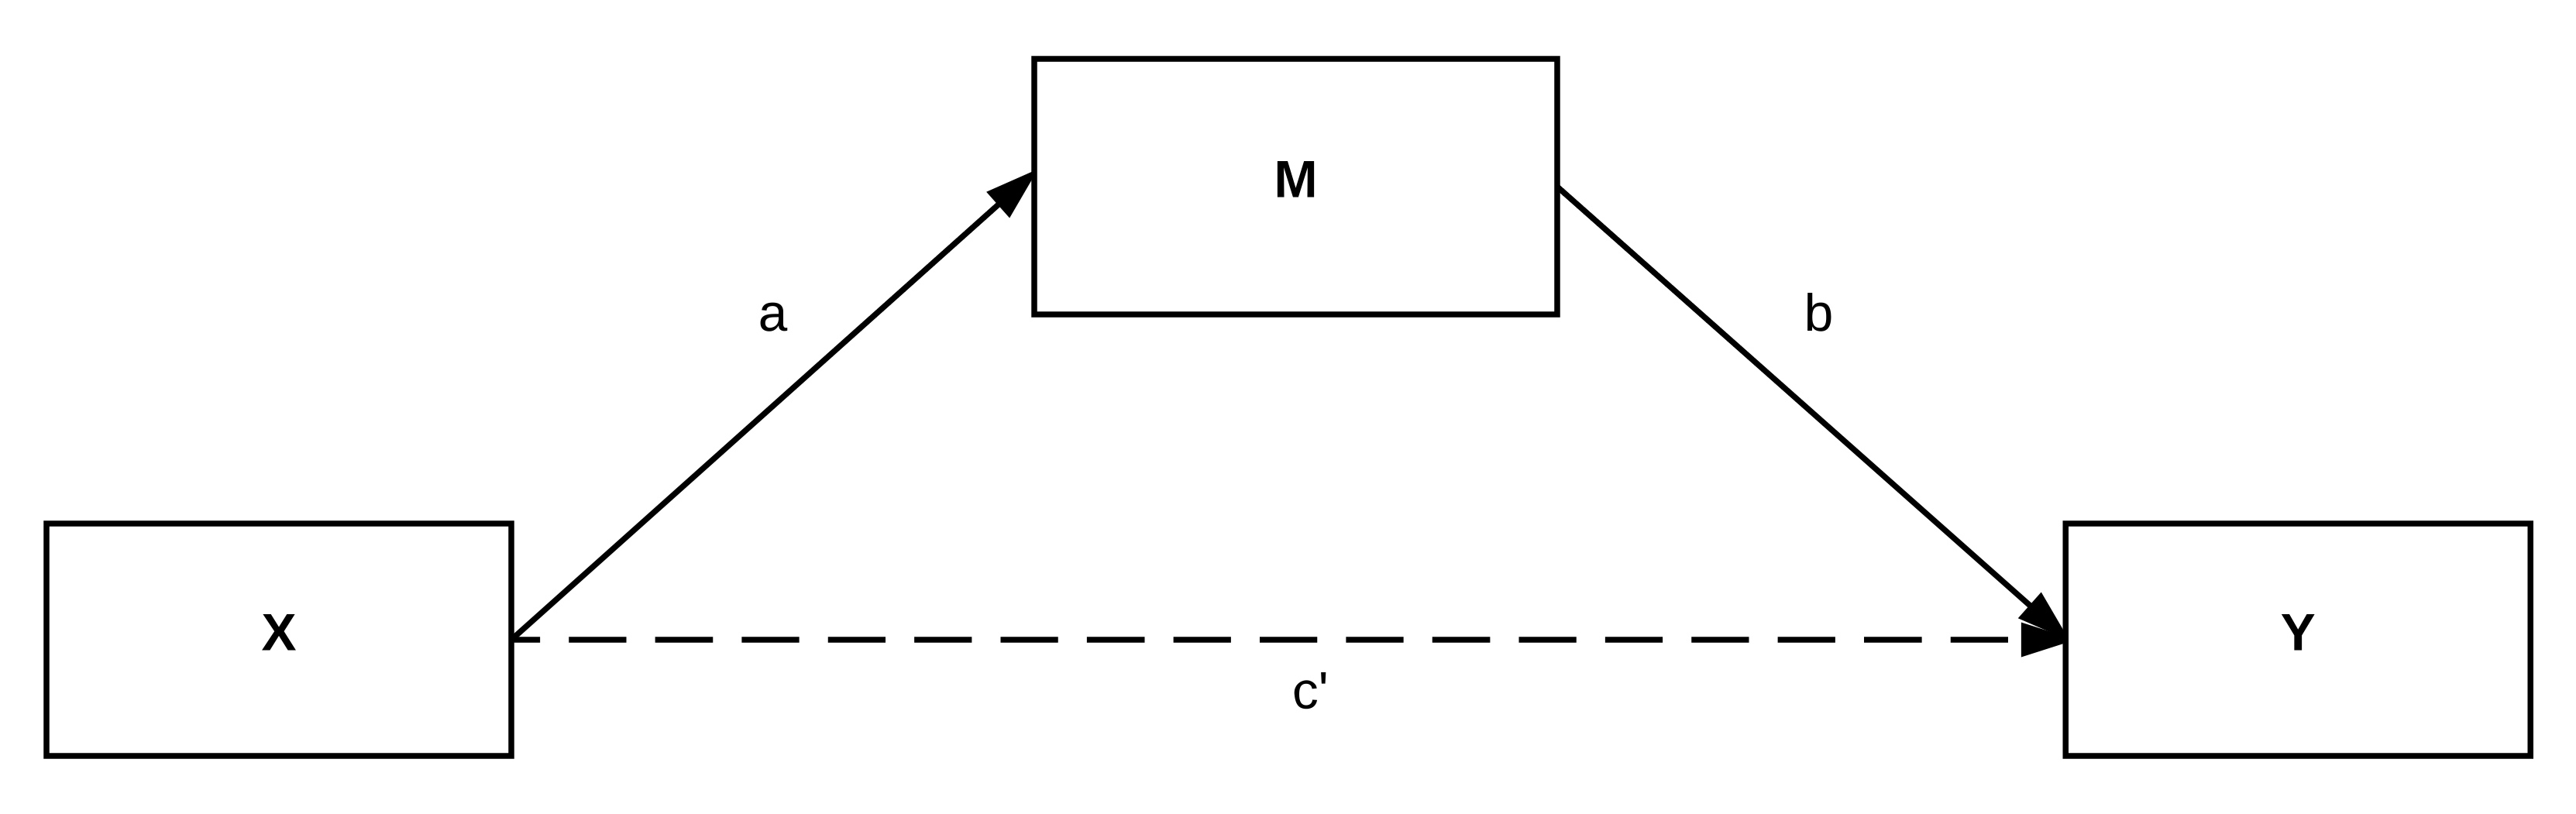
\includegraphics[width=100mm]{figures/Fig_SimpleMediation.jpg}
  \caption{Path diagram of a simple mediation analysis model with a single predictor, a single mediator, and a single outcome.}
  \label{fig:simplemed}
\end{figure}

\subsection{Definitions}\label{definitions}

Before discussing mediation further, it is helpful to note some
terminology that are often used in the field. In Figure
\ref{fig:simplemed}, X is a predictor or an exogenous variable (i.e., a
variable that is not predicted or influenced by something in the model;
``independent variable'') while M and Y are mediators and outcomes,
respectively. These are also known as endogenous variables (i.e.,
variables that are, in part, predicted or influenced by other variables
in the model). These distinctions are useful as the frameworks and
assumptions of the models are discussed.

\section{Frameworks}\label{frameworks}

Two highly related frameworks exist to perform mediation analysis
(Iacobucci, 2008). First, as mentioned previously, mediation analysis
can be built on linear regression including ordinary least squares (OLS)
and generalized linear modeling (GLM; Hayes, 2009, 2013). This requires
separate models for the \(a\) paths and the \(b\) and \(c'\) paths, fit
independently, to be combined into one mediation model. This approach is
flexible in terms of the types of variables and model specifications as
compared to the other---structural equation modeling (SEM). For example,
performing moderated mediation is more straightforward in this framework
(Edwards and Lambert, 2007; Hayes, 2013) than in SEM. Ultimately, the
regression-based framework is what this project builds upon.

Under the SEM paradigm, all the paths are simultaneously estimated,
sometimes providing more statistical power (Iacobucci,
2008).\footnote{The idea that SEM is "superior" to the regression paradigm was refuted by Hayes (2013) by noting that in most situations differences in the estimation is extremely minor and will not alter the conclusions. This can be seen in the small effect sizes presented in Iacobucci et al. (2007). Further, additional assumptions inherent in the SEM approach may not hold, although some are not easily tested (e.g., multivariate normality). With this said, SEM still provides a powerful framework for mediation analysis.}
This approach notably allows more testing of the full model fit and can
easily include latent variables but assumes, in general, that all
variables are continuous with a multivariate normal distribution. This
is a strict assumption that is difficult to assess. However, it has
extensions allowing for categorical (generally ordinal) variables to be
included, although this changes the estimation procedure. The issues
relating to categorical mediators/outcomes are discussed in the
``Analytic and Interpretation Issues with Mediation Analysis'' section.

\section{Assumptions}\label{assumptions}

In his 2008 book ``Introduction to Mediation Analysis,'' MacKinnon
(2008) discusses the
assumptions\footnote{The assumptions described herein are for both the regression and SEM frameworks for mediation, although, as noted above, SEM has a few additional assumptions as well.}
of the mediation modeling procedure. Of these primary assumptions, note
that there are no major differences from the assumptions of regression
analysis.

\begin{enumerate}
\def\labelenumi{\arabic{enumi}.}
\tightlist
\item
  \emph{Correct Functional Form}. In general, mediation assumes a linear
  relationship between predictors and mediators/outcomes. This can be
  adjusted using transformations or, more pertinently, generalized
  linear models (e.g., logistic regression). MacKinnon (2008) also
  points out that it is assumed the relationships are additive; if they
  are not, then the correct interactions (moderators) need to be
  included in the model specification. This, in many ways, needs to be
  driven by theory and prior literature (Lockhart et al., 2011).
\item
  \emph{No Omitted Influences}. A key to any mediation analysis is that
  variables that: 1) correlate with both the predictor and the mediator
  (path \(a\)), 2) correlate with both the mediator and the outcome
  (path \(b\)), or 3) correlate with both the predictor and the outcome
  (path \(c'\)) are included in the model. A more general form of this
  assumption has been termed ``sequential ignorability'' (Imai, Keele,
  and Tingley, 2010a). This more general form includes a sensitivity
  analysis to assess how important deviations from this assumption are
  on the conclusions (Imai et al., 2010a; Imai, Keele, and Yamamoto,
  2010b).
\item
  \emph{Accurate Measurement}. Random measurement error produces
  attenuated paths (in large sample sizes) and random bias (in small
  sample sizes) in regression (Loken and Gelman, 2017) and therefore can
  affect the paths in various ways (e.g., attenuate the \(b\) path which
  can inflate the \(c'\) path). When possible, reliable measures and/or
  proper latent variable modeling should be used for this assumption to
  be met.
\item
  \emph{Well-Behaved Residuals}. The residuals are assumed to be random,
  ``have constant variance at each value of the predictor variable'' and
  ``residual error terms are uncorrelated across equations'' (pg. 55).
  The assumption about uncorrelated errors can stem from ``No Omitted
  Influences'' for, if there are omitted variables in both equations,
  the error terms will correlate. This is one of the few assumptions
  that can be investigated in many situations.
\end{enumerate}

With the addition of \emph{temporal precedence} (predictor comes before
mediator) and \emph{appropriate measurement timing} (the mediator is
measured at the appropriate time when the effect of the predictor has
occurred), the resulting estimates are asymptotically (i.e., with a
large enough sample size) unbiased, allowing proper (causal) inference
regarding the effects' magnitude and direction (MacKinnon, 2008). This
interpretation, to aid in reproducibility, needs to be highlighted with
the associated uncertainty (e.g., confidence intervals) in a meaningful
metric.

\subsection{Other Considerations}\label{other-considerations}

\subsubsection{Causality}\label{causality}

To discuss causality in mediation analysis, one should be familiar with
the \emph{counter-factual} framework (or sometimes referred to as the
potential outcomes framework; Hofler, 2005). As Imai et al. (2010a)
states: ``the causal effect \ldots{} can be defined as the difference
between two potential outcomes: one that would be realized {[}in the
intervention{]} and the other that would be realized if {[}not in the
intervention{]},'' (pg. 3). In other words, the causal effect is the
difference in potential outcomes depending on the predictor (e.g., an
intervention). In reality, only one such outcome is observed---if
individual ``i'' is assigned to the treatment group, we only observe the
outcome from the treatment group and not from the control group. Imai et
al. (2010a) continues: ``Given this setup, the causal effect of the
{[}intervention{]} can be defined as \(Y_i(1) - Y_i(0)\). Because only
either \(Y_i(1)\) or \(Y_i(0)\) is observable \ldots{} researchers often
focus on the identification and estimation of the average causal
effect.'' If the conditions are randomly assigned, this is simply
\(E(Y_i(1) - Y_i(0))\), or the expected value across multiple
individuals and/or observations.

The counter-factual framework helps clarify causality in mediation
analysis by defining the necessary conditions. Using this framework,
Imai et al. (2010b) demonstrated that \emph{sequential ignorability}
(essentially the assumption that there are no omitted influences) is
required for a causal interpretation in mediation analysis. However,
this assumption is difficult to assess. Because of this difficulty, Imai
et al. (2010a) developed a general mediation model that allows a
researcher to assess how deviations from it, via sensitivity analysis,
affect the estimates.

As will be shown, the present project incorporates the counter-factual
framework intuitively. Because of its importance, this will be discussed
more in the next chapter.

\subsubsection{Modeling}\label{modeling}

Shrout and Bolger (2002) highlight a number of other important
considerations in mediation analysis. First, multi-collinearity can
produce problems, especially when it occurs between predictors and
mediators. It can distort the statistical power of the analysis,
potentially producing misleading results. The second consideration is
suppression: ``Suppression occurs when the indirect effect
\(a \times b\) has the opposite sign of the direct effect,'' (pg. 430).
This can, if not interpreted correctly, produce confusing estimates
(e.g., a positive indirect path and a negative direct path).

Shrout and Bolger (2002) also recommend using bootstrapping (also Hayes,
2009, 2013) to understand the variability in the estimates. This is due
to the asymmetric distribution of indirect effects (see Figure 6 in
Shrout and Bolger, 2002) that boostrapping can handle naturally.
Bootstrapping uses repeated random sampling of the data with replacement
and estimates the model on that sampled data. Generally, between 500 and
10,000 bootstrapped samples are used to get an accurate confidence
interval. In regards to mediation analysis, bootstrapping produces as
accurate (or more accurate) Type-I error rates than other methods in
mediation analysis. Because of this, bootstrapping plays a major role in
this project.

Two other considerations should be made regarding mediation analysis.
First, only the predictors can be randomized (i.e., the mediator cannot
be randomized in most situations). That is, even when the \(a\) and
\(c'\) paths can portray an experimental manipulation, the \(b\) path(s)
cannot. Therefore, the need for proper covariates, interpretation,
reporting, and replication is even more important in mediation analysis.
David MacKinnon said it well: ``It is not likely that a true mechanism
can be demonstrated in one statistical analysis. \ldots{} These analyses
inform the next experiment that provides more information,'' (MacKinnon,
2008, pg. 67). Therefore, the conceptual model must be considered
carefully in light of theory, prior literature, and proper covariates
(Lockhart et al., 2011). Iacobucci (2008) also recommends to evaluate
competing models and theories---thus presenting the effects and paths in
light of alternative model specifications.

Even when done properly, replication of mediated effects is important
(MacKinnon, 2008). To help make the replications most useful, the
interpretation---comprising the magnitude and direction of the
effect---needs to be reported with the proper uncertainty and include
information on a) bivariate correlations, b) information on all relevant
paths (even non-significant ones), c) must include information on the
process of variable and covariate selection, d) report standardized and
unstandardized results, and e) provide de-identified data and code {[}if
possible{]}. It is important to note that much of this information can
be included as supplemental material. In this way, results are reported
that can be combined with others in order to provide ``convincing
evidence of {[}or lack of{]} a mediating mechanism'', (MacKinnon, 2008,
pg. 67).

Second, interpretation is built on combining multiple estimates, and
often subsequently comparing those combinations with other estimates.
For example, the indirect effect is a combination of the \(a\) and \(b\)
paths and is often compared with the \(c'\) path. Therefore, if either
of the \(a\) or \(b\) paths are in units that cannot be easily combined,
the interpretation quickly becomes very difficult (see ``Analytic and
Interpretation Issues with Mediation Analysis'' section). This is
particularly true when the mediator(s) and/or outcome is non-normal.

This second hurdle, that of interpretation, is particularly important in
this project. Below, the general interpretation guidelines are
discussed, followed by when these guidelines are not straightforward.

\section{Interpretation}\label{interpretation}

In linear models, the interpretation is simple, straightforward and
intuitive. The \(a\) path coefficient means: ``for a one unit change in
X there is an associated \(a\) units change in the mediator.'' Likewise,
the \(b\) path coefficient means: ``for a one unit change in M there is
an associated \(b\) units change in the outcome, controlling for the
effect of X.'' Finally, the \(c'\) path is: ``for a one unit change in
X, controlling for the effect of M, there is an associated change of
\(c'\) units in the outcome.'' The indirect effect is \(a \times b\);
the total effect is \(a \times b + c'\).

Each element of the mediation (i.e., the indirect, the direct, and total
effects and also the individual \(a\), \(b\), and \(c'\) paths) needs to
be considered without only trying to answer: ``Is there a mediated
effect?'' Otherwise, researchers can lose sight of the complete story.
For example, the various \(a\) paths may be important on their own
(e.g., if the \(a\) path effect size is small then maybe the predictor
is not a beneficial place to focus an intervention even though the
effect is significant). Therefore, understanding a mediated effect is
best told through several avenues: the indirect, direct, and total
effects; the individual paths; these effects and paths in light of
covariates; among others. This approach is also best if those effects
are in meaningful and intuitive metrics.

However, once the analysis ventures into non-normal, non-linear
relationships, the interpretation becomes more difficult---particularly
when it comes to the indirect and total effects. For example, if the
mediator is binary, often logistic regression is used to assess the
\(a\) path. But that changes the \(a\) path interpretation to: ``for a
one unit change in X, there is an associated \(a\) log odds units change
in the mediator.'' This interpretation is anything but intuitive. In
general, the log odds are transformed into odds ratios, which improve
the interpretation. But these units do not mix well with other units.
This is detrimental to understanding the indirect and total effects as
will be discussed further in the sections below.

\section{Analytic and Interpretation Issues with Mediation
Analysis}\label{analytic-and-interpretation-issues-with-mediation-analysis}

\subsection{Categorical and Non-Normal
Mediators/Outcomes}\label{categorical-and-non-normal-mediatorsoutcomes}

Mediation analysis is more difficult when the mediator and/or the
outcome is not continuous, including binary variables (e.g., an
individual either uses marijuana or not), ordinal variables (e.g., the
self-reported confidence in social settings), other polytomous variables
(e.g., sub-types of a disease), and count variables (e.g., number of
hospital visits). These data situations are difficult because mediation
analysis requires the mediators and/or outcomes to be continuous and
approximately normal (to meet the assumption of well-behaved residuals).

There are several strategies taken in the literature to address this
problem. However, each makes its own set of assumptions and each
contains limitations in interpretation. The variability in approaches
and the subsequent interpretations make combining results across studies
far more difficult---reducing the chance to concretely show
relationships via meta-analyses and systematic reviews. The difficulty
of these data situations are likely reducing reliability and
interpretability for a number of reasons:

\begin{itemize}
\tightlist
\item
  It may be easier to ignore the assumptions that are violated when
  using categorical mediators and/or outcomes. Results from these
  analyses may not be valid.
\item
  Different approaches produce varying assumptions and interpretations.
  This can be difficult for other researchers, clinicians, lawmakers,
  and laypersons to keep in mind, possibly leading to misunderstandings
  regarding results and their validity.
\item
  Analyses with categorical outcomes are not typically well-emphasized
  in graduate training, even in more simple modeling techniques, not to
  mention more complex techniques like mediation analysis. With fewer
  individuals well-trained, more errors are likely in analyzing these
  data.
\item
  The interpretation regarding analyses with categorical outcomes is
  often far less intuitive than with continuous outcomes. This can
  produce a higher cognitive load for both the researchers and those
  utilizing the study.
\end{itemize}

With this in mind, the following subsection discusses the current
approaches to mediation analysis with categorical mediators and/or
outcomes and the assumptions these approaches make.

\subsection{Current Approaches}\label{current-approaches}

\begin{quote}
``The quest for sound methods of incorporating categorical variables is
perhaps the last dilemma in mediation analysis that lacks a strong
solution---it's the `final frontier,'\,'' (Iacobucci, 2012, pg. 583).
\end{quote}

Although there are possibly other ``frontiers'' in mediation analysis,
categorical mediators and/or outcomes certainly produce several
challenges. Iacobucci (2008, 2012) thoroughly discusses the issues of
assessing categorical variables within a mediation analysis and some of
the current practices along with their associated
problems\footnote{For the present, only situations when a mediator or outcome is categorical is under consideration since a categorical predictor poses very few problems (Iacobucci, 2012).}.
Four approaches are of note here: 1) a series of logistic regression
models, 2) polychoric correlation in SEM, 3) the method suggested by
Iacobucci (2012) regarding standardization, and 4) interpreting each
path separately. A fifth, but certainly least, is to ignore the
distribution of the outcomes and purposefully misspecify the model.
These are highlighted in Table \ref{tab_approaches}.

\begin{table}[tb]
\centering
\caption{The various approaches to handling mediation with categorical mediators/outcomes.} 
\label{tab_approaches}
\begin{tabular}{p{40mm}p{45mm}p{55mm}}
\toprule
Approach & Pros & Cons \\ 
\midrule
1. Series of logistic regressions & Simple to apply in most software & Cannot obtain indirect effect size, only useful in few situations \\ 
2. SEM's approach (polychoric correlation) & Powerful, well-designed, Easy to implement with proper software & Only works with ordinal variables, only standardized effect sizes \\ 
3. Standardize the coefficients & Provides significance test of indirect effect & Assumptions regarding distributions, difficult to interpret beyond p-value \\ 
4. Interpret each path separately & Simplest approach with proper models & Ignores some information, cannot obtain indirect effect size \\ 
5. Pretend all variables are continuous & Simplest approach & Purposeful mis-specification, poor model fit \\ 
\bottomrule
\end{tabular}
\end{table}

Of these approaches, only the SEM approach allows any proper estimation
of effect sizes. This approach was developed by Muthén (1984), which
uses polychoric correlations (for ordered categorical variables) within
the structural equation modeling framework. In this approach, Muthén
(1984) assumes that the ordered categorical manifest variable results
from a continuous latent variable, ``with observed categorical data
arising through a threshold step function,'' (Iacobucci, 2012, pg. 583).
In many cases, a continuous latent variable is a reasonable assumption.
For example, in a binary variable describing whether an adolescent has
ever smoked marijuana, assuming a continuous latent variable comprised
of the probability of smoking may adequately represent reality. This
method relies on using a probit regression ``to model the relationship
between the observed categorical variable and the latent \emph{normally
distributed} variable,'' (MacKinnon, 2008, pg. 320, emphasis added) and
requires large sample sizes (Iacobucci, 2008). Using this
latent-observed sub-model, the probit is used as the threshold value to
estimate the full model. Notably, both the assumption of a normally
distributed latent variable and the requirement of large sample sizes
are limitations of this approach.

The other approaches, including the series of logistic regression models
and the interpretation of each path separately, do not allow any effect
size estimation of indirect effects. Although there are some ways to
discuss the proportion of mediation (Ford and Hill, 2012), this still
does not provide any measures of effect size. The third approach,
recommended by Iacobucci (2012), proposed using a new standardization
solution using logistic regression output (for a categorical variable)
that can combine linear and logistic models' estimates. It is built on
the same idea as the Sobel test (MacKinnon, 2008; Sobel, 1982) but is
more flexible; for ``the mechanics of testing for mediation do not
{[}need to{]} change whether the variables are continuous or categorical
or some mix,'' (Iacobucci, 2012, pg. 593). However, MacKinnon and Cox
(2012) criticized this approach. Ultimately, the most fatal flaw may be
that a focus on the significance (relying on Null Hypothesis
Significance Testing) of the effects without regard to their effect size
in meaningful terms is less interpretable and impactful.

In the end, none of these approaches can flexibly handle categorical
variables of various kinds (e.g., binary, multinomial) or other
non-normal distributions (e.g., costs, counts); none can produce
intuitive and meaningful effect sizes and confidence intervals across
these variable types; and none can consistently combine two differing
types of estimates (e.g., binary mediator with continuous outcome, count
mediator with binary outcome). Although the current approaches are
useful in some situations---particularly the SEM approach---a more
complete framework is needed.

\section{Conclusions}\label{conclusions}

Mediation analysis is a powerful framework for understanding the
processes by which one variable influences another. The assumptions are
not much more than that of regression analysis. The interpretation, in
linear models, is straightforward and simple. However, once the analysis
ventures into non-normal, non-linear relationships, the interpretation
becomes more difficult---particularly when it comes to the indirect and
total effects.

In the end, Iacobucci (2012) is correct in saying this problem ``lacks a
strong solution'' (pg. 583). Although important information can be
obtained from the current methods, mediation analysis with categorical
mediator(s) and/or outcome(s) still misses the mark on intuitive,
meaningful effect sizes.

This project aims to alleviate these issues by integrating a
post-estimation approach known as \emph{Average Marginal Effects} (AMEs)
within mediation analysis. This integration can allow simple and
meaningful interpretation across variable types and combinations thus
far shown to be problematic. The following chapter introduces AMEs,
showing their benefit in interpretation and reporting when working with
non-normal variables within generalized linear models.

\singlespacing

\FloatBarrier

\newpage

\fancyhead[L]{Average Marginal Effects} \fancyhead[R]{\thepage}
\fancyfoot[C]{}

\chapter{AVERAGE MARGINAL EFFECTS}

\begin{quote}
\emph{Any fool can know. The point is to understand.}
--- Albert Einstein
\end{quote}

\doublespacing

\section{Introduction}\label{introduction-1}

When the outcome variable is not continuous and/or has a distribution
far from normal, researchers in prevention science often rely on
generalized linear models (GLMs). The power of GLMs is clear when you
consider the broad range of situations it estimates with asymptotic
consistency.\footnote{Asymptotic consistency refers to the ability to, as the sample size increases, produce estimates that converge to the proper value.}
However, the problem with GLMs is that the estimates are not in an
easily interpretable form. For example, in logistic regression (one type
of GLM), the results are in ``log-odds''. To overcome this lack of
interpretability, a simple exponentiation of the coefficient produces
what is known as an odds ratio. Similarly, Poisson regression (another
form of GLM), with an exponentiation, produces the risk ratio. Although
some fields have adopted odds ratios (or relative risk, risk ratios, and
other related metrics), these metrics have notable shortcomings.

\begin{enumerate}
\item Most of these metrics can be difficult to understand (i.e., many are not intuitive).
\item They cannot be combined with other metrics in a meaningful manner.
\end{enumerate}

First, data have suggested that individuals, although with some
variability, are able to intuitively grasp the meaning of phrases such
as ``highly probable'' or ``not likely'' (Heuer Jr., 1999). Yet, this
same intuition is not found in odds or odds ratios. For example,
Montreuil, Bendavid, and Brophy (2005) found, of 84 articles in several
epidemiology journals that used odds ratios, only 7 (8.3\%) accurately
interpreted the odds ratio and 22 (26\%) interpreted odds as though they
were probabilities (``risk''). Figure \ref{fig:orprob} highlights the
large discrepancy between the odds ratio, the risk ratio, and the
average marginal risk. Ultimately, reporting odds and interpreting them
as risk is common.

The second is particularly important in the case of mediation analysis
given the importance of the indirect effect (the combination of the
\(a\) and \(b\) paths). If \(a\) is not in a unit that can be combined
with \(b\), then obtaining a meaningful indirect effect is not generally
possible. Given its commonality and the limitation that it cannot be
combined with other metrics, it is time to consider other
strategies---at least in some situations.

\begin{figure}[tb]
  \centering
  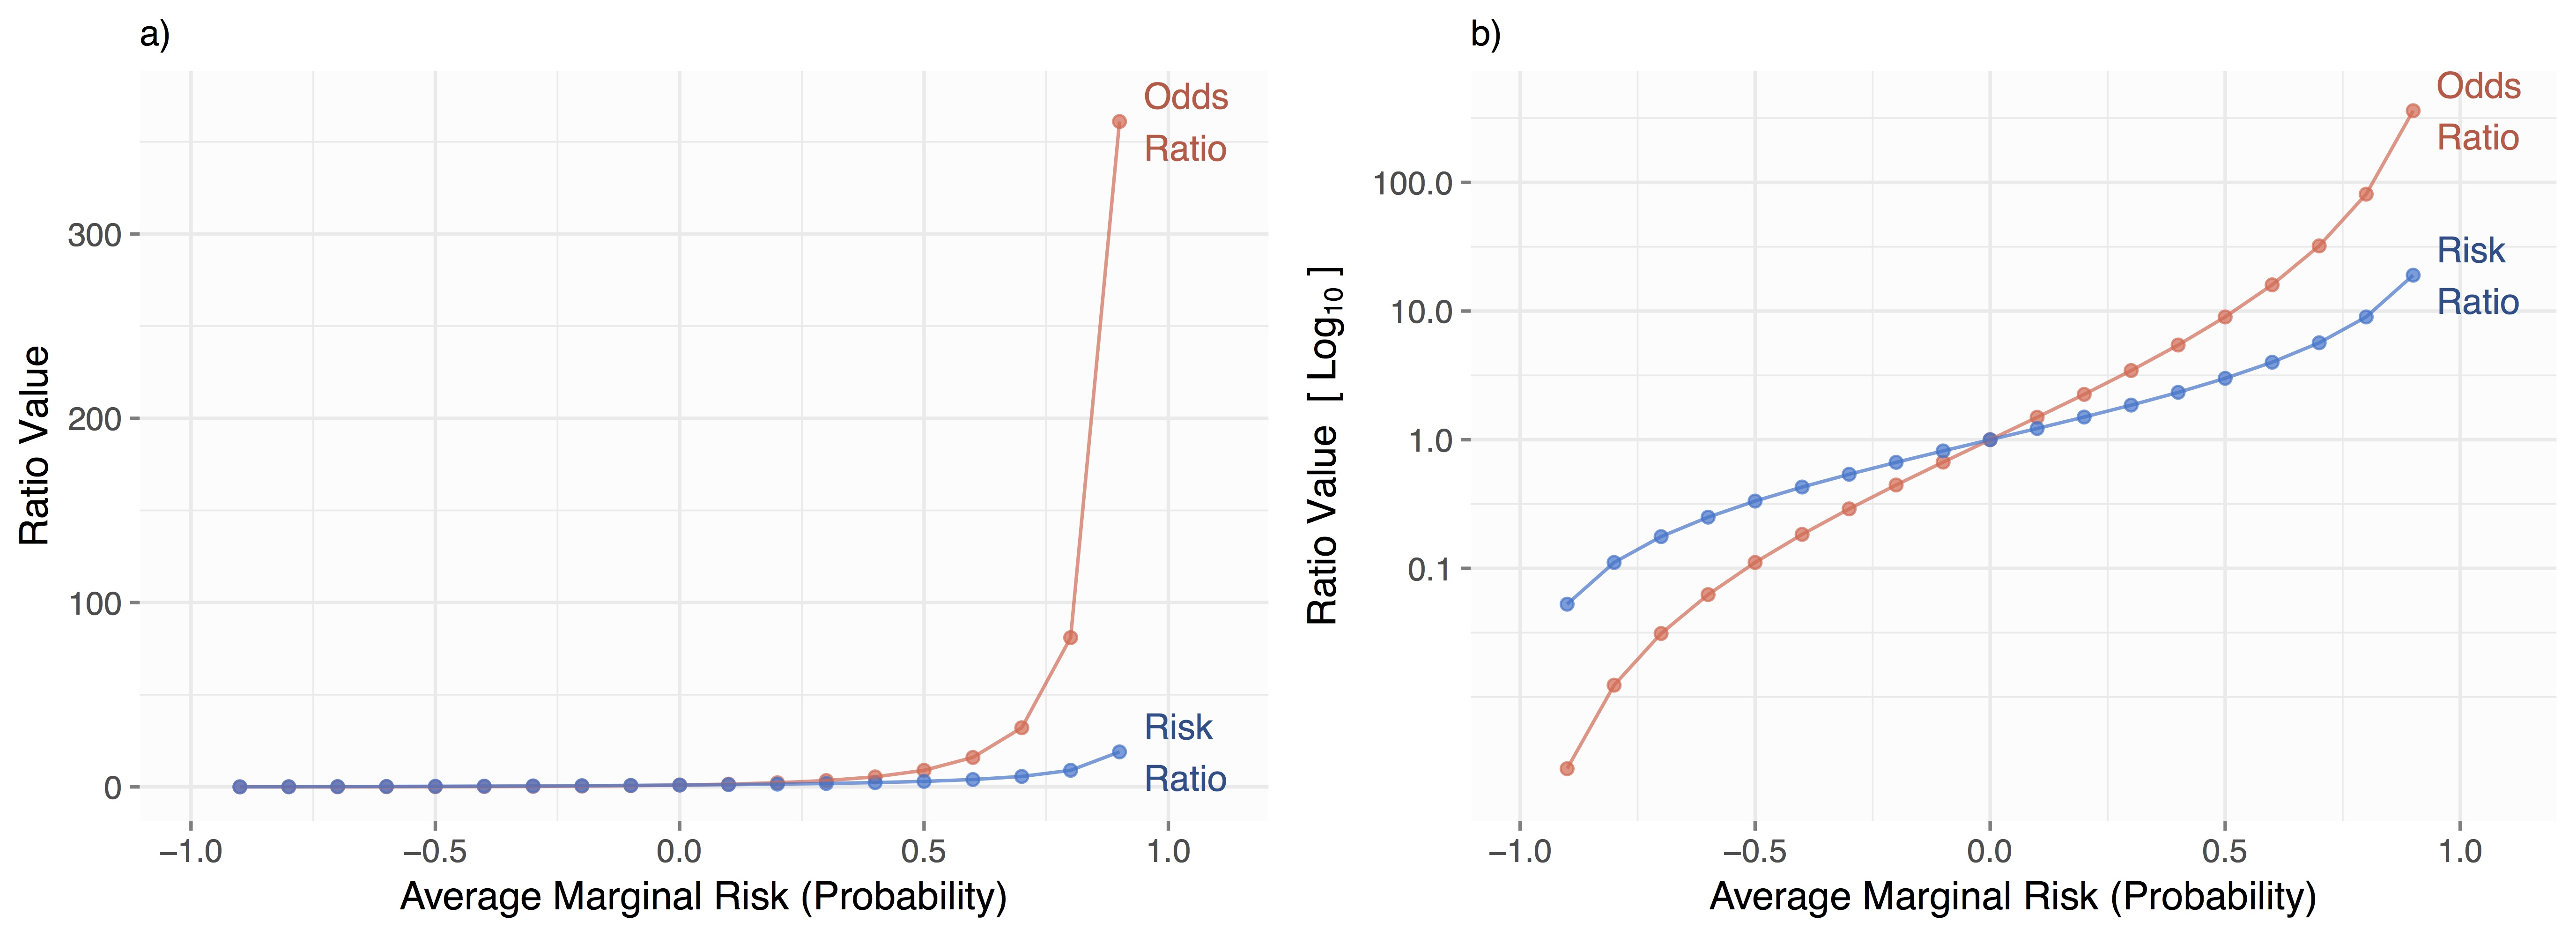
\includegraphics[width=\linewidth]{figures/OR_Prob.jpg}
  \caption{a) Comparison of odds ratio and risk ratio with the average marginal risk (probability). b) Same comparison as a) but the y-axis is rescaled ($log_{10}$) to better show the negative marginal risk comparisons. Both highlight the discrepancy between odds and risk ratios at various levels of marginal risk and that neither approximate the marginal risk.}
  \label{fig:orprob}
\end{figure}

\section{Additive vs.~Multiplicative
Interpretations}\label{additive-vs.multiplicative-interpretations}

The distinction between additive and multiplicative estimates is
generally important but is particularly so in mediation analysis. In
most quantitative research designs, the investigators are seeking
information on the average effect in a population, whether this refers
to an average difference across groups or an average change in the
outcome for a given change in the predictor. Generally speaking, the
average effect is referring to the marginal effect (i.e., the effect of
a small change in the predictor in the outcome's units). In the linear
regression framework, the average effect is the estimated coefficient
and is interpreted \emph{additively}---a one unit change in the
predictor is associated with an X unit change in the outcome.
Conversely, outcomes such as OR are \emph{multiplicative}. Being
multiplicative changes the interpretation to: a one unit change in the
predictor is associated with an X times change in the outcome. Although
subtle, the difference is important, especially for multi-part models
(e.g., mediation analysis).

Being multiplicative indicates that the effect of the predictor changes
based on the level of the predictor. For example, if the predictor is
high, a small change in the predictor may have a big effect while if the
predictor is low, a small change in the predictor has little effect.
Figure \ref{fig:loglinear} shows this phenomenon, where, in the outcomes
original units there is an exponential function. In part a) of the
figure, it is clear that a change from 2 to 3 in the predictor has a
much larger effect than a change from 0 to 1. A regression would not
work well here. If a log transformation is used, the relationship would
be linear (and a regression can be used) but the interpretation becomes
multiplicative (in this case a one unit increase in the predictor is
associated with an \(X*100\) percent increase in the outcome).

\begin{figure}[tb]
  \centering
  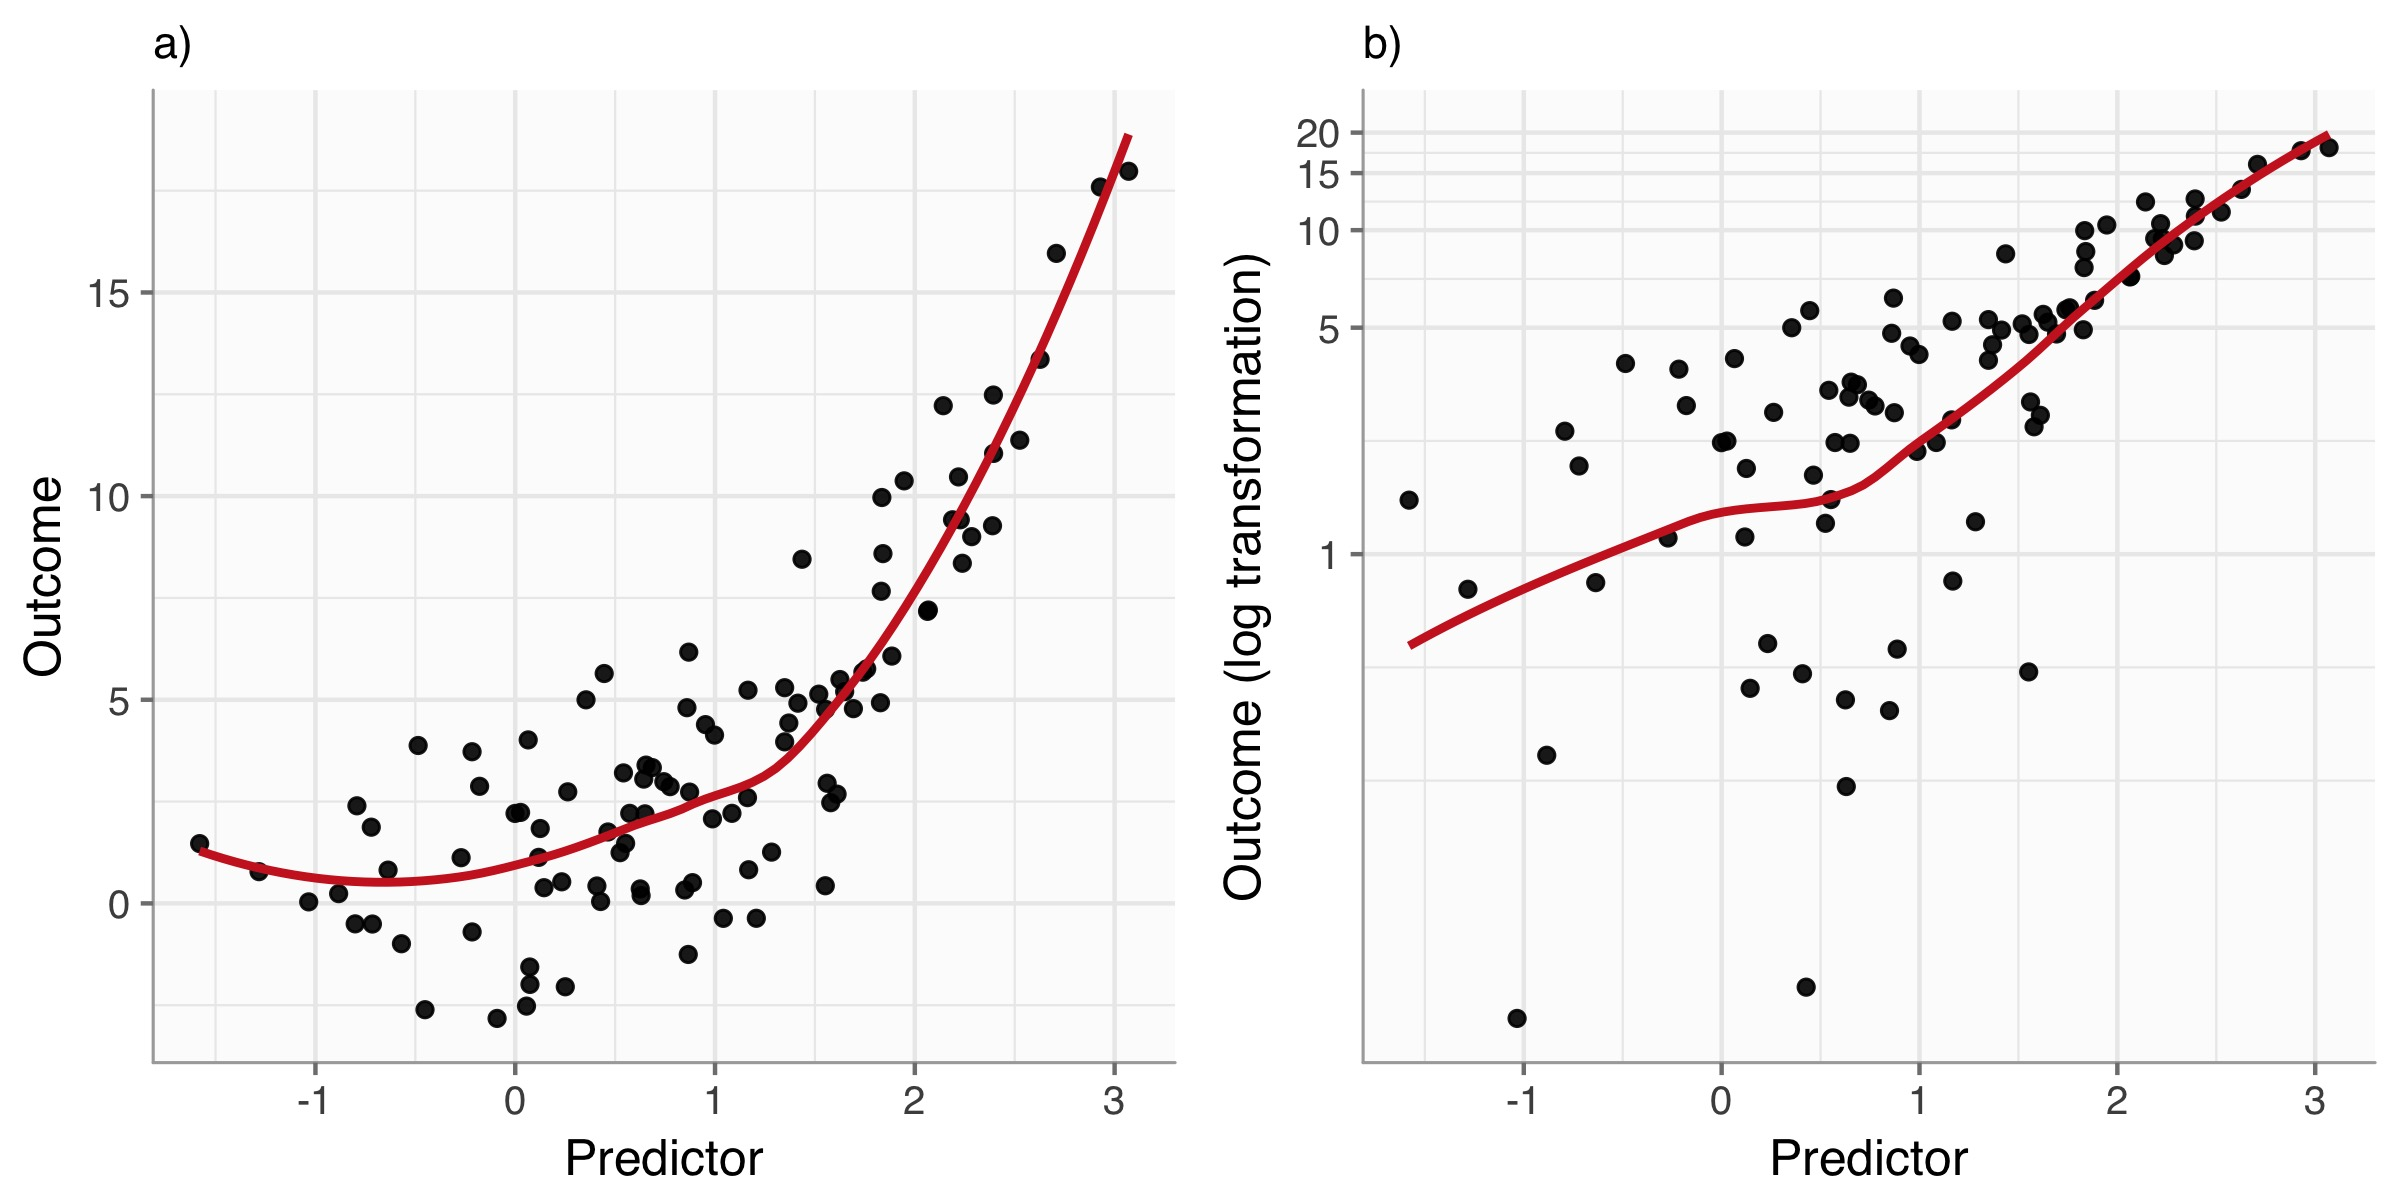
\includegraphics[width=\linewidth]{figures/loglinear.jpg}
  \caption{Demonstration of a non-linear relationship. a) The outcome is an exponential function of the predictor. b) When log transforming the outcome, the relationship becomes fairly linear. So the interpretation in the log transformed scale is additive, but once it is put back into the original units, it is multiplicative.}
  \label{fig:loglinear}
\end{figure}

Additive interpretations are generally the most intuitive and require
less cognitive resources to understand the pattern being portrayed. In a
multiplicative framework, simplicity in understanding the effect
intuitively is somewhat lost (Iacobucci, 2008). Among others, this is
one reason why Stata provides the \texttt{margins} command when dealing
with two-part hurdle
models.\footnote{These models are often used for zero-inflated count outcomes.}
These models break up the modeling into two parts: one for the binary
part and one for the count part. In order to combine the two parts,
Stata allows a transformation known as the \emph{average marginal
effect} (AME) that makes the two parts both additive, and therefore
easily combined (as is also desired in mediation analysis).

\section{Average Marginal Effect}\label{average-marginal-effect}

\subsection{Why Consider Average Marginal
Effects?}\label{why-consider-average-marginal-effects}

When using GLMs, the model is fit with a link function (e.g., ``logit'',
``probit'', ``log''). This change causes the marginal effect of a
variable to rely on the values of the covariates in the model. This is
well illustrated through an example. Say a logistic regression model was
fit to the data, as shown in Equations \ref{logisticmodel} -
\ref{logisticmodel4}, for \(p\) predictors.

\begin{equation}\label{logisticmodel}
logit(Y_i) = \beta_0 + \sum_{j=1}^p \beta_{j} X_{ij} + \epsilon_i
\end{equation}\begin{equation}\label{logisticmodel2}
log(\frac{Prob(Y_i = 1)}{1 - Prob(Y_i = 1)}) = \beta_0 + \sum_{j=1}^p \beta_{j} X_{ij} + \epsilon_i
\end{equation}\begin{equation}\label{logisticmodel3}
\frac{Prob(Y_i = 1)}{1 - Prob(Y_i = 1)} = e^{\beta_0 + \sum_{j=1}^p \beta_{j} X_{ij} + \epsilon_i}
\end{equation}\begin{equation}\label{logisticmodel4}
Prob(Y_i = 1) = \frac{e^{\beta_0 + \sum_{j=1}^p \beta_{j} X_{ij} + \epsilon_i}}{1 + e^{\beta_0 + \sum_{j=1}^p \beta_{j} X_i + \epsilon_i}}
\end{equation}

\noindent This implies that the marginal effect of, say, \(X_{i1}\) is:

\begin{equation}\label{marginallogistic}
\frac{\delta Y}{\delta X_1} = \frac{e^{\beta_0 + \sum_{j=1}^p \beta_{j} X_{ij} + \epsilon_i}}{(1 + e^{\beta_0 + \sum_{j=1}^p \beta_{j} X_{ij} + \epsilon_i})^2}
\end{equation}

\noindent That is, the marginal effect of the predictor \(X_1\)
\emph{depends} on the level of each covariate for each individual (all
\(X_{ij}\)'s) and each estimate (all \(\beta_j\)'s). This,
understandably, complicates the interpretation.

Importantly, this example makes it clear that each observational unit
(e.g., individual) has a unique marginal effect given her observed
levels of each variable. For example, if variable \(X\) is increased by
one from wherever it was observed, each individual will have different
effects (i.e., different marginal effects). One individual may have a
large effect; another small. Each individual has a marginal effect of a
given predictor associated with her set of characteristics (covariates).
To understand the average effect in the population of interest, the mean
of all such marginal effects can be calculated.

The AME, then, is the \emph{averaged} marginal effect across all
observational units in the data. In linear models, the AME is the same
as the original model estimates. This is intuitive given the AME is the
marginal effect in the outcome's original units---the exact
interpretation of the estimates in a linear model. However, as stated
previously, in GLMs the estimates are not in the original units and
therefore must be estimated via a post-estimation calculation described
below.

\subsection{Definition of the Average Marginal
Effect}\label{definition-of-the-average-marginal-effect}

In an instructive paper about the (now defunct) routine called
``margeff'' in Stata, Bartus (2005) highlights how the AME can be
calculated---including the mathematical definition---and the benefits of
AMEs compared to other related methods. The AME is a post-estimation
calculation---it uses the model estimates and the data to provide the
average effect. Bartus (2005) provided the definition of this
post-estimation procedure of a continuous predictor as:

\begin{equation}
AME_{k} = \beta_k \frac{1}{n} \sum_{i=1}^n f(\beta X)
\end{equation}

\noindent where \(f\) refers to the probability density function of
\(F\), \(\beta X\) is the linear combination of the predictors (i.e.,
the model predicted values for each observation), and \(AME_k\) is the
average marginal effect for the \(kth\) variable. This definition
provides the average change in the outcome for a one unit change in the
continuous variable \(x_k\) across all \(n\) observations.

Relatedly, the AME of a dummy coded variable is:

\begin{equation}
AME_{k} = \frac{1}{n} \sum_{i=1}^{n} \big[ F(\beta X | x_{ki} = 1) - F(\beta X | x_{ki} = 0) \big]
\end{equation}

\noindent where \(F(\beta X | x_{ki} = 1)\) is the predicted value of
the \(ith\) observation when the dummy variable \(x_k\) equals one and
\(F(\beta X | x_{ki} = 0)\) is the predicted value when the dummy value
of \(x_k\) equals zero holding all other variables constant. This, in
effect, shows the discrete difference between the levels of the
categorical variable in the outcome's original units.

\subsection{Confidence Intervals}\label{confidence-intervals}

In general, two approaches are taken to estimate the confidence
intervals of AMEs. The first approach is the delta method, which
provides standard errors (StataCorp, 2015). Although beneficial, the
second---bootstrapped confidence intervals---have proven accurate for
understanding the variability in both the AME and mediation analysis.
Therefore, this project uses bootstrapped confidence intervals.

\subsection{The Counter-Factual
Framework}\label{the-counter-factual-framework}

As mentioned previously, this project---including the use of average
marginal effects---fits within the counter-factual framework. Indeed,
the definition of a dummy coded variable demonstrates this
well---\(\big[ F(\beta X | x_i = 1) - F(\beta X | x_i = 0) \big]\). In
essence, this answers the question: ``What is the difference in the
outcome when all observations of \(x_k\) are equal to one vs.~when all
observations of \(x_k\) are equal to zero?'' The counter-factual
framework strives to answer the same class of questions. When all
assumptions are met, the AME is a direct, statistical answer to the
causality conditions proposed by this framework.

\section{Interpretation}\label{interpretation-1}

Table \ref{tab_int} presents the various units that the AME will produce
for the various GLM links. It is important to note that AMEs are in the
outcome's original metrics whether they are probabilities, counts, or
something else. The interpretation, then, is ``for a one unit change in
the predictor there is an associated {[}AME{]} change in the outcome.''

\begin{table}[tb]
\centering
\caption{The generalized linear model link functions with their associated units of interpretation. Note: This list is not exhaustive and there are likely more GLMs that are used within prevention research.} 
\label{tab_int}
\begin{tabular}{lc}
\toprule
Link Function & Average Marginal Effect \\ 
\midrule
Identity & Original Continuous Unit \\ 
  Log & Original Continuous Unit \\ 
  Logit & Risk \\ 
  Probit & Risk \\ 
  Poisson & Count \\ 
  Gamma & Count \\ 
  Negative Binomial & Count \\ 
\bottomrule
\end{tabular}
\end{table}

\subsection{Benefits and Limitations}\label{benefits-and-limitations}

There are several benefits to using average marginal effects with GLMs.

\begin{itemize}
\item \emph{Intuitive Interpretation and Few Assumptions}. The first, and most obvious, benefit to using AMEs is the simplicity of the interpretation. The effect is in the units used in the modeling; it is additive (i.e., the effect is the added increase or subtracted decrease in the outcome). It provides an interpretation that imitates that of ordinary least squares regression. Relatedly, there are no difficult modeling assumptions directly tied to AMEs. Instead, the underlying models' assumptions that are used to get the AME is what is important. The only additional assumption with AME is that the effect, for each individual, is linear enough to be represented by an additive value and that the average adequately reports this.
\item \emph{More Generalizable and Robust}. There is evidence suggesting that AMEs are more robust to problems associated with GLMs (including logistic regression) such as unobserved heterogeneity and model mis-specification (Mood, 2010; Norton, 2012). This allows the estimates to be more generalizable to individuals outside of the sample.
\item \emph{Low Computational Burden}. Given AMEs are a post-estimation calculation, no new models need to be fit. Instead, using the estimates of the models, the average marginal effects can be calculated. The most computationally expensive aspect of the calculation is the bootstrapped confidence intervals. 
\item \emph{Broadly Applicable}. The AME applies to any of the generalized linear models including logistic, Poisson, gamma, beta, negative binomial, and two-part hurdle models. This provides extensive flexibility in modeling, and, once applied to mediation, will allow flexibility in modeling based on the correct functional form.
\item \emph{Two-Part Models}. Particularly pertinent to this project is that the calculation of AMEs have been applied to two-part models, generally of the hurdle model types, as stated earlier. In fact, this is a common routine in the Stata statistical software. This provides valuable support for the proposed approach of using AMEs in mediation analysis.
\end{itemize}

Notably, the interpretation of AMEs hold to the assumption (as found in
all regressions) that it is reasonable to adjust a single covariate
while holding all others constant. This may not hold in reality,
although it may be necessary to gain an understanding of the individual
effect of a single variable. In data that are not representative of the
population (e.g., non-random sample), AMEs may be biased because an
over-representation of certain covariate values may be present. This is
an overall modeling problem, since GLMs also assume a random sample. In
this way, this problem is not specific to AMEs.

\section{Conclusions}\label{conclusions-1}

The Average Marginal Effect produces intuitive, interpretable, and
additive estimates of an effect. They have been applied to two-part
models, similar to mediation analysis, demonstrating their utility in
difficult modeling situations. The following chapter discusses the
integration of AME with mediation analysis---termed \emph{Marginal
Mediation Analysis}--- with its interpretation and assumptions, its
benefits and limitations, and the basic procedures for its use.

\singlespacing

\FloatBarrier

\newpage

\fancyhead[L]{Marginal Mediation Analysis} \fancyhead[R]{\thepage}
\fancyfoot[C]{}

\chapter{MARGINAL MEDIATION ANALYSIS}

\begin{quote}
\emph{Without an interpretable scale, it is difficult to use effect size to communicate results in a meaningful and useful way.}
--- Preacher and Hayes, 2011
\end{quote}

\doublespacing

\section{Introduction}\label{introduction-2}

The proposed integration of average marginal effects and mediation
analysis is designed to resolve two major obstacles currently found in
mediation analysis:

\begin{enumerate}
\def\labelenumi{\arabic{enumi}.}
\tightlist
\item
  The difficulty of performing mediation analysis with categorical
  mediators and/or outcomes, and
\item
  The lack of reliable and flexible effect size estimates in mediation
  analysis---particularly with categorical mediators and/or outcomes.
\end{enumerate}

\noindent These issues are relatively common in prevention work (e.g.,
Ford and Hill, 2012; B. Hoeppner, Hoeppner, and Abroms, 2017; Wong and
Brower, 2013) and the current approaches are not adequate---as was
discussed at length in the previous chapters. In this chapter, the
integration of Average Marginal Effects (AMEs) and mediation
analysis---\emph{Marginal Mediation Analysis} (MMA)---is discussed,
including its interpretation and assumptions as well as its benefits and
limitations. It is expected that this adjustment to both the modeling
and the interpretation will help researchers in the health and
prevention sciences to be able to model their data in the most
properly-specified way and be able to communicate their findings
clearly.

\section{Definition of Marginal Mediation
Analysis}\label{definition-of-marginal-mediation-analysis}

The form of the general marginal mediation model, including the
post-estimation step, are demonstrated in the following equations, where
Equations \ref{equation_a} and \ref{equation_b} demonstrate the
mediation estimation while Equations \ref{equation_AMEa} and
\ref{equation_AMEb} show the post-estimation procedures.

\begin{equation}\label{equation_a}
M_{ij} = a_0 + \sum_{k=1}^p a_k x_{ki} + \epsilon_i \text{ }\text{ }\text{ for j = 1, ..., m mediators}
\end{equation}\begin{equation}\label{equation_b}
Y_{i} = \beta_0 + \sum_{j = 1}^m b_j M_{ij} + \sum_{k=1}^p c_k^{'} x_{ki} + \epsilon_i
\end{equation}

\noindent for the \(ith\) individual, for \(k = 1, ..., p\) predictors,
and \(j = 1, ..., m\) mediators. The paths are all labeled with their
common term (e.g., path \(a\) is labeled \(a\)). Combining these two
equations provides the full mediation model. Using these models, we
apply the post-estimation of the average marginal effects as presented
by Bartus (2005). For a continuous \(x_k\) variable, the average
marginal effect of path \(a\) is:

\begin{equation}\label{equation_AMEa}
AME^a_k = a_k \frac{1}{n} \sum_{i=1}^n f(a X)
\end{equation}

\noindent where \(f\) refers to the probability density function,
\(a X\) is the linear combination of the predictors (i.e., the model
predicted values for each observation), and \(AME_k^a\) is the average
marginal effect of the \(a\) path for the \(kth\) variable. Ultimately,
Equation \ref{equation_AMEa} is identical to that of the following:

\begin{equation}\label{equation_AMEa1}
AME^a_k = \frac{1}{n} \sum_{i=1}^n \frac{f(aX_1) - f(aX_2)}{2h}
\end{equation}

\noindent where

\begin{equation}\label{equation_AMEa2}
aX_1 = \begin{bmatrix}
ax_{11} & ax_{12} & \dots & ax_{1k} + h & \dots & ax_{1p} \\
ax_{21} & ax_{22} & \dots & ax_{2k} + h & \dots & ax_{2p} \\
\vdots  & \vdots  & \ddots & \vdots     & \ddots  & \vdots \\
ax_{n1} & ax_{n2} & \dots & ax_{nk} + h & \dots & ax_{np}
\end{bmatrix}
\end{equation}

\noindent and

\begin{equation}\label{equation_AMEa3}
aX_2 = \begin{bmatrix}
ax_{11} & ax_{12} & \dots & ax_{1k} - h & \dots & ax_{1p} \\
ax_{21} & ax_{22} & \dots & ax_{2k} - h & \dots & ax_{2p} \\
\vdots  & \vdots  & \ddots & \vdots     & \ddots  & \vdots \\
ax_{n1} & ax_{n2} & \dots & ax_{nk} - h & \dots & ax_{np}
\end{bmatrix}
\end{equation}

\noindent Both \(f(aX_1)\) and \(f(aX_2)\) are the model predicted value
for the outcome given the small change due to \(h\). Equations
\ref{equation_AMEa1}, \ref{equation_AMEa2}, and \ref{equation_AMEa3} use
a very small \(h\) value (default is \(1 \times 10^{-7}\)). This
provides the change in the average predicted value for a very small
increase and a very small decrease in in the \(x_k\) variable. This is
also described in depth by Leeper (2017) since it is the strategy
employed by \texttt{margins}. This approach is flexible---especially in
the R statistical environment with the improvement of derivative
computation that Leeper provided.

Similarly, the AME of a dummy coded variable in the \(a\) path is:

\begin{equation}\label{equation_AMEb}
AME_{k}^a = \frac{1}{n} \sum_{i=1}^{n} \big[ F(a X | x_{ki} = 1) - F(a X | x_{ki} = 0) \big]
\end{equation}

\noindent where \(F(a X | x_{ki} = 1)\) is the predicted value of the
\(ith\) observation when the dummy variable equals one and
\(F(a X | x_{ki} = 0)\) is the predicted value when the dummy value
equals zero. This is the same approach used by \texttt{margins}.

Notably, these same post-estimation equations (\ref{equation_AMEa} and
\ref{equation_AMEb}) can be used for the \(b\) and \(c'\) paths as well.

\section{Interpretation}\label{interpretation-2}

The interpretation of Marginal Mediation is based on the original units
of the mediator(s) and outcome(s). Because there are so many possible
combinations of GLM types within mediation analysis, instead of
outlining every combination, the basic principles are presented that
apply to all situations.

\subsection{Principle 1: The individual paths are interpreted based on
the corresponding endogenous variable's original
metric.}\label{principle-1-the-individual-paths-are-interpreted-based-on-the-corresponding-endogenous-variables-original-metric.}

The individual paths have interpretations identical to those of AMEs, as
discussed in Chapter 2. Therefore, the \(a\) path depends on the type of
mediator and modeling approach chosen. For example, for a binary
mediator, the \(a\) path is a probability (risk); a mediator
representing a count has an \(a\) path that is in the same count units.

\subsection{\texorpdfstring{Principle 2: The indirect effect, as a
combination of the \(a\) and \(b\) paths, are interpreted based on the
outcome's original
metric.}{Principle 2: The indirect effect, as a combination of the a and b paths, are interpreted based on the outcome's original metric.}}\label{principle-2-the-indirect-effect-as-a-combination-of-the-a-and-b-paths-are-interpreted-based-on-the-outcomes-original-metric.}

The indirect effect is joining two paths, possibly of different metrics.
However, the interpretation is still straightforward: the entire effect
will be in the outcome's original metric. An example may be beneficial
to highlight this principle.

Suppose there are data with a hypothesized binary mediator (depression
or no depression) and a continuous outcome (quality of life). A logistic
regression is used to model path \(a\) and a linear regression is used
for the \(b\) and \(c'\) paths. After calculating the AME of the paths,
path \(a\) is in units of risk (of depression) while path \(b\) is the
difference in the quality of life between depressed and not depressed
individuals. By combining paths \(a\) and \(b\) through multiplication,
we get the effect of the predictor on depression risk then what that
depression risk does to quality of life; that is, the effect of the
predictor on quality of life through depression.

\subsection{Principle 3: Both the direct and total effects are
interpreted based on the outcome's original
metric.}\label{principle-3-both-the-direct-and-total-effects-are-interpreted-based-on-the-outcomes-original-metric.}

Similar to Principle 2, the direct and total effects are in the
outcome's original units. This is intuitive given that the AME of the
direct effect is in the outcome's units, and it is not combined with any
other path. For the total effect, the indirect and direct effect (which
are both in the same units) are added together to get the complete
effect. It was expected that, as in linear regression (but that is
lacking in other situations), \(a \times b + c'= c\). That is, the
indirect and direct effects together equals the total effect. This
expectation was tested, as is described in the next chapter.

\subsection{Effect Sizes}\label{effect-sizes}

A major advantage of this framework is the way effect sizes can be used
intuitively.

\begin{quote}
``First, virtually all effect size indices should be scaled
appropriately, given the measurement and the question of interest.
Without an \emph{interpretable scale}, it is difficult to use effect
size to communicate results in a meaningful and useful way\ldots{}.
Second, it should be emphasized that effect size estimates are
themselves sample statistics and thus will almost certainly differ from
their corresponding population values. Therefore, it is important to
report confidence intervals for effect sizes\ldots{}'' (Preacher and
Kelley, 2011, pg. 95, emphasis added).
\end{quote}

The interpretation of MMA makes it clear that both of these aspects of
proper effect size estimation and reporting are adequately represented.
Of particular note, unlike many effect sizes that are only useful in
certain research questions, the effect sizes produced by AMEs---and thus
found in Marginal Mediation Analysis---are flexibly oriented to ``be
scaled appropriately'' to best ``communicate results in a meaningful and
useful way'' for a wide variety of situations.

Additionally, Preacher and Kelley (2011) continue: ``it is important to
develop a way to gauge the effect size of the product term \(ab\)
itself,'' (pg. 95). That is, not only does the effect size of the
individual paths need to be meaningful but the product of \(a \times b\)
must be as well. Marginal Mediation Analysis provides this comparability
as the indirect effect can be compared without problems with the direct
and total effects (they are all in the same units).

\section{Assumptions}\label{assumptions-1}

The assumptions inherent in MMA are the same as those presented in
Chapter 1 regarding mediation analysis. The only additional assumption
regards the ability of the effect to be represented additively (i.e.,
can the effect be represented linearly after accounting for the marginal
effect for each observation?). In linear models, this is already
included as an implicit assumption. For other models, although the
relationship may not be linear in the outcome, taking the average of the
effects across the observations is assumed to be representative of the
relationship across the sample.

\section{Reproducibility and
Interpretability}\label{reproducibility-and-interpretability}

As mentioned previously, categorical mediators/outcomes are generally
not difficult to model using GLMs---only the interpretation is
difficult. Generalized linear models, in conjunction with AMEs, allow
researchers to use more correct functional forms, thereby reducing the
justification to fit poorly specified models that have an easier
interpretation.

With this framework, MMA can be applied across the GLM spectrum and
essentially any combination of GLM types. For example, a marginal
mediation model is defined when the mediator is binary and the outcome
is continuous; when the mediator is a count and the outcome is ordinal;
when the mediator is continuous and the outcome is binary. Each has a
straightforward, yet informative, interpretation as outlined by the
principles above. This attribute alone can increase the reproducibility
of research using mediation analysis.

Finally, the interpretation across the paths and effects is
straightforward and flexible. Other researchers, laypersons, lawmakers,
and clinicians can assess the direction, magnitude, meaning, and utility
of findings much easier---thus, increasing the reach and impact of
research. In mediation analysis, this can prove largely beneficial given
the already complex nature of the modeling scheme. By simplifying the
interpretation, less cognitive resources are required to gain a basic
understanding of the findings; instead, more resources can be used to
understand how to apply it and assess future research questions based on
the findings.

\singlespacing

\FloatBarrier
\newpage
\fancyhead[L]{Methods} \fancyhead[R]{\thepage} \fancyfoot[C]{}

\chapter{METHODS}

\begin{quote}
\emph{For precept must be upon precept, precept upon precept; line upon line, line upon line; here a little, and there a little.}
--- Isaiah 28:10, King James Bible
\end{quote}

\doublespacing

\section{Introduction}\label{introduction-3}

As presented in the previous chapter, Marginal Mediation Analysis (MMA)
has the ability to simplify the interpretation of mediated effects in a
wide variety of situations, particularly in situations where an effect
size otherwise does not exist (e.g., indirect effects when the mediator
or outcome is categorical). In this chapter, methods fashioned to
develop MMA and evaluate its performance are discussed via three phases:

\begin{enumerate}
\def\labelenumi{\arabic{enumi}.}
\tightlist
\item
  Development of MMA
\item
  Monte Carlo Simulation Study of MMA
\item
  Application of MMA
\end{enumerate}

\noindent These phases were designed to provide the theory and the
software to perform MMA, assess the method's ability to accurately
estimate the underlying effects, develop the guidelines of its use in
finite samples, and apply it to real-world prevention data by
replicating a recent study (Ford and Hill, 2012) that used a categorical
mediator and categorical outcomes. Below, each phase is described in
depth.

\section{Phase I: Development of Marginal Mediation
Analysis}\label{phase-i-development-of-marginal-mediation-analysis}

To be useful to public health, psychological, and prevention
researchers, the incorporation of average marginal effects within
mediation analysis must happen in two ways: in theory and in software.
This phase is focused on understanding the properties of MMA and on
developing the software necessary to perform it.

\subsection{Properties of MMA}\label{properties-of-mma}

Building on the mediation framework discussed by Hayes (2009) and by
Edwards and Lambert (2007), MMA was established on linear
regression---either ordinary least squares (OLS) for continuous
outcomes/mediators or maximum likelihood (via GLMs) for categorical
outcomes/mediators. In this framework, two or more regression equations
are combined to provide the overall mediation model as discussed in
Chapter 1. This method then adds a post-estimation step (Chapter 2) into
this mediation framework.

The form of the general marginal mediation model, including the
post-estimation step, were discussed in Chapter 3. Using this general
framework, various considerations were made in the development of the
method. First, an appropriate manner in which to integrate moderation
(interaction effects) into the framework is important. Because of the
work by Edwards and Lambert (2007), this included assessing the
\emph{reduced
form}\footnote{Reduced form refers to only having exogenous variables on the right-hand side of a regression equation (i.e., substituting the predictors of the mediators into the equation).}
of the models in addition to visualizations of the predicted values
across levels of the moderator. Second, it has been noted by MacKinnon
(2008) that in non-linear models the \(a \times b + c'\) generally does
not equal the \(c\) path as it does in linear models (Chapter 11 in his
book). To assess whether these are equal within MMA, both a basic
analysis and a Monte Carlo simulation (phase II) was used.

\subsection{Software Development}\label{software-development}

A major aspect of this first phase is the development of the software
for researchers to apply MMA. This software is provided via the R
statistical environment given R is free, widely used by researchers in
health and prevention, and extensions to the software via ``packages''
are efficiently disseminated through the Comprehensive R Archive Network
(CRAN). It consists of a number of functions to fit the model and assess
the model's fit while efficiently producing the paths and effects in
proper units.

Because of the flexibility of numerical derivation methods and the speed
improvements by Thomas Leeper (2017), numerical derivatives were used to
obtain the marginal effects for each observational unit. From here,
means of the marginal effects were calculated for each variable in the
model. To assess the model uncertainty, bootstrapping via the
\texttt{boot} R package was applied. This approach relies on repeated
resampling from the original sample \emph{with replacement}. In general,
this method does not rely on any distributional assumptions and works
well with asymmetric distributions (as is found in indirect effects).

The package applies the best practices for both computational speed and
user readability (Wickham, 2015), allowing other researchers to extend
the package more easily. Additionally, several built-in tests will
inform the functionality of the package before beginning Phase 2. These
tests were performed on Linux, Mac, and Windows platforms. Finally, the
package uses Git as the version control system. The necessary functions
were developed first so that the package tests and simulations could
begin. The usability of the package that is important in the
disseminated version were developed afterwards.

\section{Phase II: Monte Carlo Simulation Study of Marginal Mediation
Analysis}\label{phase-ii-monte-carlo-simulation-study-of-marginal-mediation-analysis}

The evaluation of MMA is an essential step in understanding its
properties and robustness and further assess the performance of the
software. The consistency of MMA, the statistical power at various
sample sizes, and the accuracy of the bootstrapped confidence intervals
were all tested via a Monte Carlo simulation study (Carsey and Harden,
2013; Paxton, Curran, Bollen, Kirby, and Chen, 2001).

In the simulation, data were simulated to come from a population of
known parameters. A literature review of mediation analysis in
prevention work highlighted the appropriateness of the population
parameters chosen. The results of the simulation helped in the
development of the guidelines for using MMA in practice.

\subsection{Literature Review}\label{literature-review}

Before performing the Monte Carlo simulations, a review of the
literature is recommended (Paxton et al., 2001). This review focused on
the use of mediation analysis in prevention research where the analyses
contained categorical mediators and/or outcomes. This review included
all recent articles (2008 - 2017) found that clearly identified a
mediator or outcome that was categorical in nature. This search relied
on terms such as ``generalized linear models'', ``logistic'',
``dichotomous'', ``polytomous'', and ``count'' in conjunction with
``mediation analysis'' across the Scopus database.

\subsection{Simulations}\label{simulations}

Monte Carlo simulations, via the R statistical environment version
3.4.2, assessed the finite properties of MMA. Monte Carlo simulation was
selected due to its simplicity in generating informative results and its
high success in the literature (e.g., Graham, Olchowski, and Gilreath,
2007; Nylund, Asparouhov, and Muthen, 2007). Here, 500 data sets were
simulated for each combination of experimental conditions (Carsey and
Harden, 2013; Paxton et al., 2001). The data were simulated from a known
population with a researcher specified causal model (i.e., the
``population model''). The model consisted of either a binary mediator
(0 = ``No'', 1 = ``Yes'') or a count variable (Poisson distribution), a
continuous outcome, and a continuous predictor while also varying the
sample size and the effect sizes for a total of 90 unique combinations
of the conditions (see Table \ref{tab_conditions}).

The \(a\) path population model is defined below for when the mediator
is binary, where the \(Prob(M_{u} = 1)\) is a latent continuous variable
with a logistic relationship with the predictors and the \(\epsilon_i\)
is normally distributed with a mean of 0 and a standard deviation of 1.

\begin{equation}
log(\frac{Prob(M_{u} = 1)_{i}}{1 - Prob(M_{u} = 1)_{i}}) = a_0 + a_1 x + \epsilon_i
\end{equation}

\noindent The observed variable, \(M_{o}\), is defined as follows:

\begin{equation}
M_{o} = \begin{cases}
            0, & \text{if } Prob(M_u = 1) < .5, \\
            1, & \text{otherwise}.
         \end{cases}
\end{equation}

The \(a\) path population model for when the mediator is a count is
shown below where \(M_u\) is a latent continuous variable with an
exponential relationship with the predictors and the \(\epsilon_i\) is
normally distributed with a mean of 0 and a standard deviation of 1.

\begin{equation}
log(M_u) = a_0 + a_1 x + \epsilon_i
\end{equation}

\noindent The observed variable, \(M_{o}\), is defined as follows:

\begin{equation}
M_{o} = Po(\lambda = M_u)
\end{equation}

\noindent This creates an observed, count variable that has \(\lambda\)
values based on the latent mediator.

The \(b\) and \(c'\) paths population model is identical to Equation
\ref{equation_b} with only one predictor and a single binary, or count,
mediator, as shown below.

\begin{equation}
M_{i} = a_0 + a_1 x_1 + \epsilon_{mi}
\end{equation}\begin{equation}
Y_{i} = \beta_0 + b M_{i} + c^{'} x_{i} + \epsilon_{yi}
\end{equation}

\begin{table}[tb]
\centering
\caption{The various experimental conditions of the Monte Carlo simulation study.} 
\label{tab_conditions}
\begin{tabular}{lc}
\toprule
Independent Variables & Conditions \\ 
\midrule
Sample size & 50, 100, 200, 500, 1000 \\ 
  Effect size of a path & small, moderate, large \\ 
  Effect size of b path & small, moderate, large \\ 
  Effect size of c' path & moderate \\ 
  Type of mediator & binary, count \\ 
  \midrule
  Total conditions & 90 \\ 
\bottomrule
\end{tabular}
\end{table}

Table \ref{tab_conditions} highlights the conditions that were varied
for each simulation. A distinct MMA model was applied to each of the 500
data sets for each possible combination of experimental conditions. This
means 45,000 MMA models were fit. Using eight cores of powerful core i7
computers, these computations were finished over a span of several days.

Notably, the effect sizes for both the binary mediator and count
mediator (a path) were the odds ratios and risk ratios corresponding to
small, moderate, and large effect sizes. These are found in Table
\ref{effectsizes}.

\begin{table}[tb]
\centering
\caption{The effect sizes of the a and b paths in the Monte Carlo Simulation.} 
\label{effectsizes}
\begin{tabular}{lccc}
%\toprule
Size & Odds Ratio (a path) & Risk Ratio (a path) & r (b path) \\ 
%\midrule
Small    & 1.58 & 1.34 & 0.10 \\ 
Moderate & 3.44 & 1.82 & 0.30 \\
Large    & 6.73 & 3.01 & 0.50 \\ 
%\bottomrule
\end{tabular}
\end{table}

The focus of the simulations was to gauge the accuracy, power, and
coverage of MMA at estimating the population effects while undergoing
the experimental conditions. The dependent variables were:

\begin{enumerate}
\def\labelenumi{\arabic{enumi}.}
\tightlist
\item
  bias (i.e., is the mean of the estimates at the population mean?),
\item
  power (i.e., how often does the null properly get rejected?),
\item
  confidence interval coverage (i.e., does the confidence interval cover
  the proper interval?), and
\item
  consistency regarding how closely \(a \times b + c'\) is to \(c\)
  (i.e., does the indirect plus the direct effect equal the total
  effect?).
\end{enumerate}

\noindent The effects of the conditions on these outcomes were assessed
via visualizations and descriptive tables.

\subsection{Guideline Development}\label{guideline-development}

Recommendations from the simulation study were documented, including
necessary sample sizes, bias in various conditions, and the accuracy of
bootstrapped confidence intervals in each condition. The documentation
will be available in manual form online on the
\href{http://www.r-project.org}{R website} and
\href{github.com}{GitHub}.

\section{Phase III: Application of Marginal Mediation
Analysis}\label{phase-iii-application-of-marginal-mediation-analysis}

During the third phase, all important aspects of MMA discovered
throughout the first two phases were used to replicate previous work
regarding the relationship of adolescent religiosity with substance use
(Figure \ref{fig:theorymed}). This study was selected given it used:

\begin{enumerate}
\def\labelenumi{\arabic{enumi}.}
\tightlist
\item
  a large sample with a mix of binary and continuous mediators and
  outcomes,
\item
  one of the better and common statistical approaches, and
\item
  data that were publicly available and that had a more recent release
  to investigate.
\end{enumerate}

\begin{figure}[tb]
  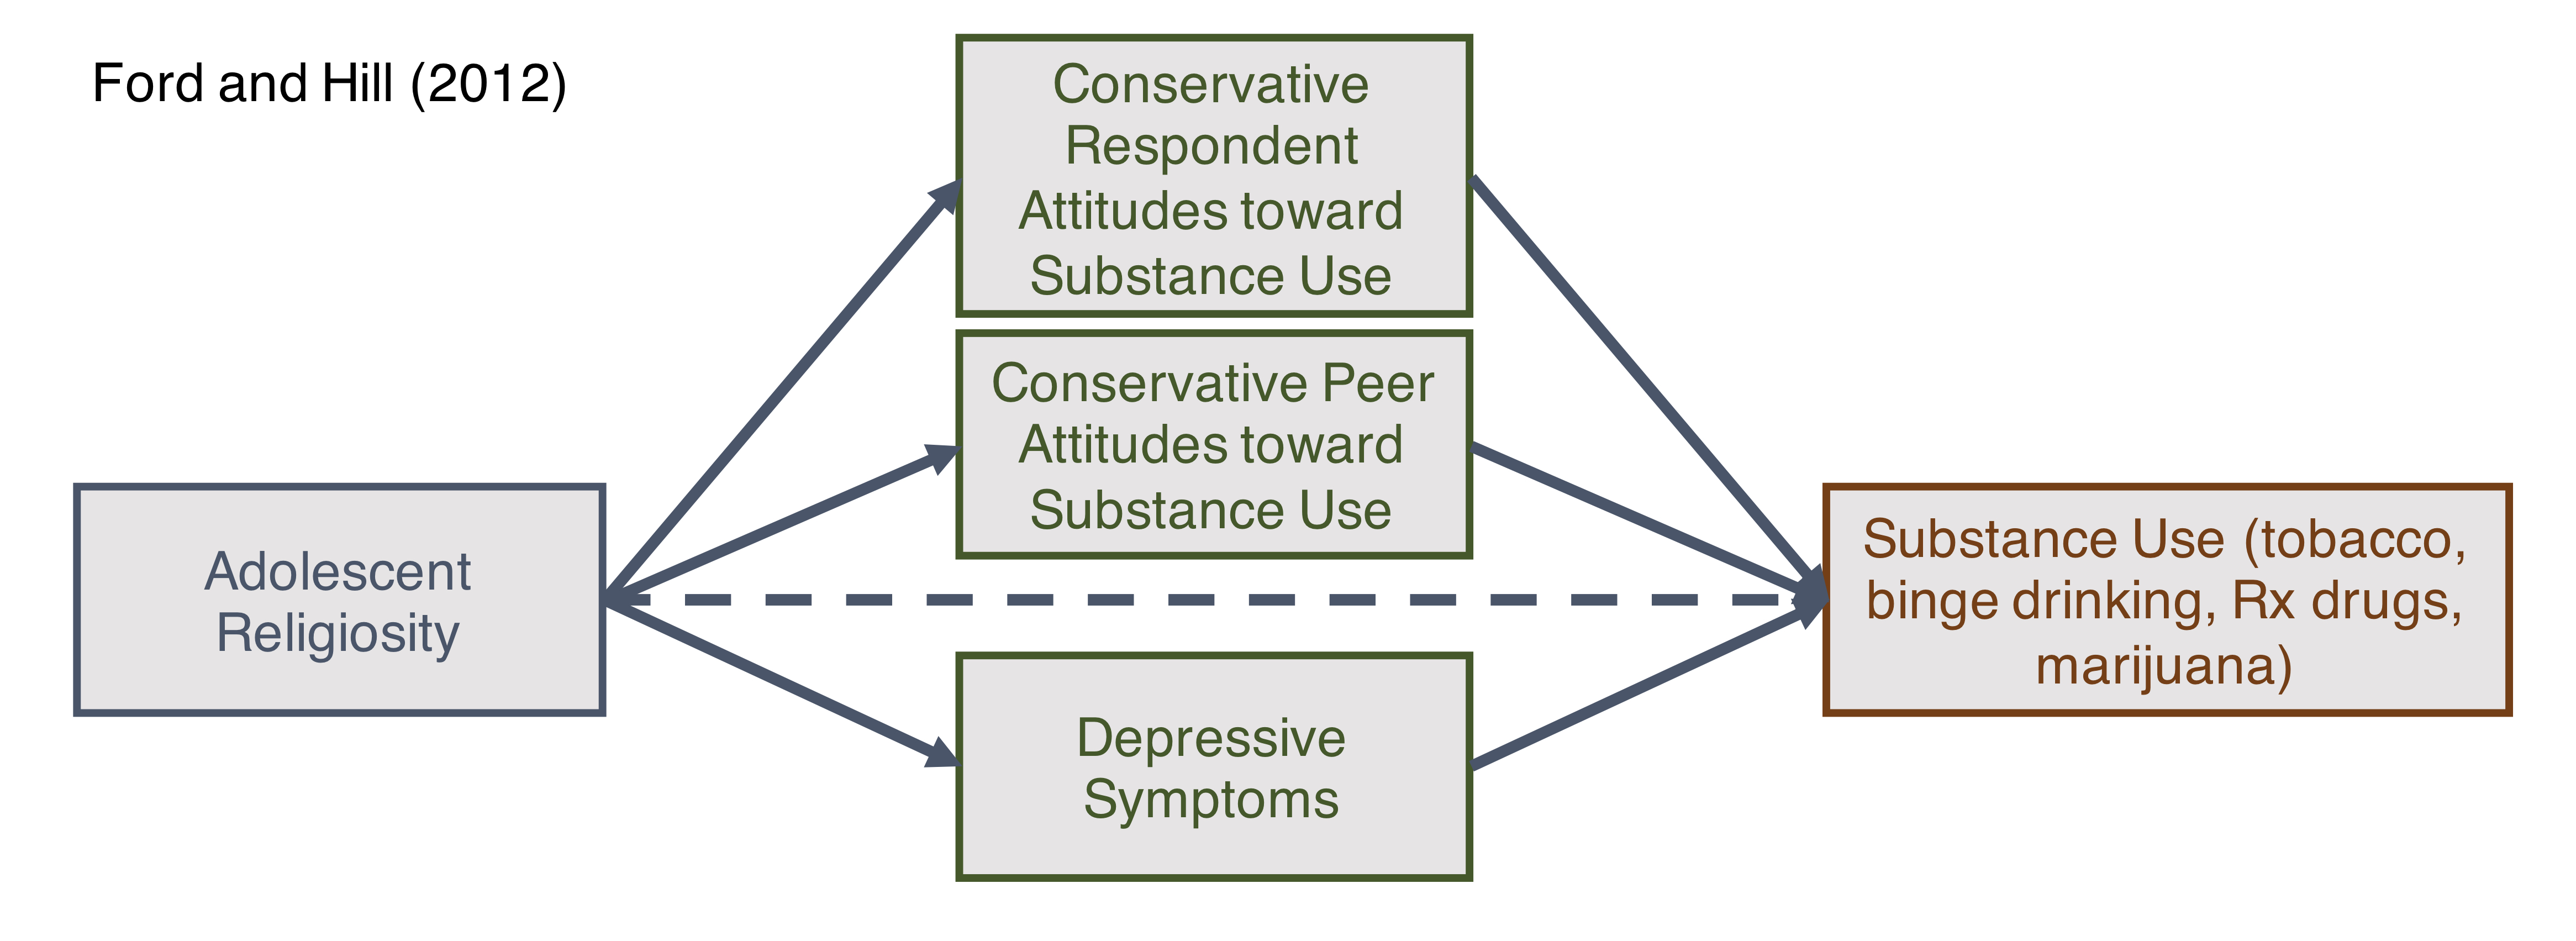
\includegraphics[width=\linewidth]{figures/fig_application_model.jpg}
  \caption{Path diagram of the replicated models from Ford and Hill (2012). The depression mediator and all of the outcomes are categorical.}
  \label{fig:theorymed}
\end{figure}

\subsection{Data}\label{data}

To replicate this study, data from the 2014 (most recent) release of
National Survey on Drug Use and Health (NSDUH; Ford and Hill, 2012) were
used. As described by Ford and Hill (2012), the NSDUH is ``an ongoing
study sponsored by the U.S. Substance Abuse and Mental Health Services
Administration that dates back to the 1970s'' (page 4) and collects data
on drug use of individuals 12 years and older across the United States.
Ford's study used the 2007 data release while the replication uses the
2014. Several
measures\footnote{Notably, this replication study omits the "heavy drinking" outcome because positive responses to it were very rare in the 2014 data.}
were used to replicate the findings of Ford and Hill (2012):

\begin{enumerate}
\def\labelenumi{\arabic{enumi}.}
\tightlist
\item
  Four substance use outcomes (tobacco use, prescription drug use,
  marijuana use, and illicit drug use).
\item
  Religiosity was based on the average response across four items
  relating to church attendance, the importance of religious beliefs to
  the individual, and participation in faith-based activities. Higher
  scores indicated more religiosity.
\item
  Respondent attitudes toward substance use was also the average
  response based on four items gauging the individual's response to
  someone their age using substances. Higher scores indicate more
  conservative attitudes.
\item
  Peer attitudes toward substance use is similar to the respondent
  attitudes except that it was asked how the individual's friends would
  feel about someone their age using substances. Again, the average
  response was used where higher scores indicate more conservative
  attitudes.
\item
  ``Psychological well-being was indicated by major depression,'' (page
  5) which was measured as at least five of the nine possible depression
  symptoms listed in the survey.
\end{enumerate}

\subsubsection{Substance Use}\label{substance-use}

As stated previously, the substance use outcomes are tobacco use,
prescription drug use, marijuana use, and illicit drug use.

\begin{itemize}
\tightlist
\item
  Tobacco use was defined as one of the following three items: 1)
  cigarette use within the last year, 2) smokeless tobacco use within
  the last year, and 3) cigar use within the last year.
\item
  Prescription drug use consisted of four groups of drugs that are being
  used either without a prescription or for the sole purpose of
  obtaining a high within the last year: pain relievers, tranquilizers,
  stimulants, and sedatives.
\item
  Marijuana use was a single item: marijuana use within the last year.
\item
  Illicit drug use was defined as using any of the following drugs
  within the last year: cocaine, crack, heroin, hallucinogens, LSD, PCP,
  ecstasy, inhalants, or meth.
\end{itemize}

\noindent Each outcome was coded as dichotomous: use or no use within
the last year.

\subsubsection{Religiosity}\label{religiosity}

Adolescent religiosity was the mean response across four items: 1) the
number of times attended religious activities in past year, 2) religious
beliefs are important, 3) religious beliefs influence decisions, and 4)
the amount of participation in religious activities. The higher the
average score the more the adolescent is considered to be religious.

\subsubsection{Respondent and Peer
Attitudes}\label{respondent-and-peer-attitudes}

The respondent's conservative views on drug use is the average of four
items, answering the question ``How do you feel about someone your age
using {[}cigarettes daily, marijuana, marijuana monthly, drinking
daily{]}?'' Similarly, the peer's conservative views on drug use is the
average of four items, answering the question ``How do you think your
close friends would feel about you using {[}cigarettes daily, marijuana,
marijuana monthly, drinking daily{]}?''

\subsubsection{Psychological Well-being}\label{psychological-well-being}

Finally, psychological well-being was defined as having had a major
depressive episode in the past year. This was a binary (yes or no)
variable based on ``if they reported experiencing at least five of the
following: felt sad, empty, or depressed most of the day or discouraged;
lost interest or pleasure in most things; experienced changes in
appetite or weight; sleep problems; other noticed you were restless or
lethargic; felt tired or low energy nearly every day; felt worthless
nearly every day; inability to concentrate or make decisions; any
thoughts or plans of suicide,'' (Ford and Hill, 2012, pg. 5).

\subsection{Analyses}\label{analyses}

The mediation analyses were replicated from Ford and Hill (2012).
Although the mediation analysis is performed differently herein, the
model specifications were identical to that employed there.

Importantly, Ford and Hill (2012) say: ``we use the categorical data
method outlined by MacKinnon (2008) to formally test the indirect
effects,'' (pg. 5). This approach uses a significance test based on the
estimates of both \(a\) and \(b\) and their standard errors. However, as
stated throughout this project, the significance alone is insufficient
information to provide for a mediation analysis; effect sizes are also
necessary. Because of this, Ford and Hill (2012) continue by discussing
the amount of the association between the predictor and outcome, in
percentage units, that the mediator accounted for. This approach is
useful but has some notable shortcomings. First, depending on the level
of multi-collinearity in the models, the standard errors of the
estimates can be inefficient which reduces the statistical power of this
test. Second, it does not provide the effect size measures that would be
most useful (e.g., the effect a one unit increase in the predictor has
on the outcome through the mediator). Third, the measure is consistently
too conservative with binary outcomes (Jiang and Vanderweele, 2015).

For the replication, then, each of the mediation models reported were
run using MMA in place of the techniques employed by Ford and Hill
(2012). Four distinct MMA models, one for each of the substance use
outcomes, were assessed. These were all controlling for (adjusting for)
parental attitudes towards substance use, age, race, sex, and income.
The models included 500 bootstrapped samples to obtain 95\% confidence
intervals.

Further, using a variant of the ``difference method,'' the amount of the
total effect that was mediated was calculated using the following: \[
\text{Proportion mediated} =\frac{indirect}{indirect + direct}
\] \noindent Finally, the information provided through the use of MMA
was also compared to that produced in the original
paper.\footnote{All analysis code is available on the Open Science Framework (osf.io/753kc) and in the Appendices of this document.}

\section{Conclusions}\label{conclusions-2}

Ultimately, the goal of this project is to develop, evaluate and apply a
method that can provide meaningful interpretation in mediation when the
mediator and/or outcome is categorical. Each phase builds on this goal,
as is discussed in the following chapters starting with the presentation
of the results of Phase I and Phase II regarding the theory, software,
and evaluation of MMA.

\singlespacing

\FloatBarrier
\newpage
\fancyhead[L]{Phase I \& II} \fancyhead[R]{\thepage} \fancyfoot[C]{}

\chapter{PHASES I \& II: DEVELOPMENT AND TESTING OF MMA}

\begin{quote}
\emph{Exploring the unknown requires tolerating uncertainty.}
--- Brian Greene
\end{quote}

\doublespacing

\section{Introduction}\label{introduction-4}

The results of both Phase I (the development of the method and its
software) and Phase II (the Monte Carlo simulations) regarding Marginal
Mediation Analysis (MMA) are presented in this chapter.

\section{Developmental
Considerations}\label{developmental-considerations}

The general MMA framework was discussed in Chapter 3. This framework was
extended with some important additional considerations, including
integrating moderation and analytically assessing the relation between
the decomposed total effect and the total effect.

\subsection{Moderation}\label{moderation}

Moderation (interaction) is sometimes hypothesized to occur in
conjunction with mediation. Moderation is any situation where the effect
of a variable on another \emph{depends} on the value of a third
variable. This phenomenon, in conjunction with mediation, is often
referred to as conditional process analysis, moderated mediation, or
mediated moderation---depending on the source and situation.

An example of one of the many possible moderated mediation models is
found in Figure \ref{fig:modmed} (for more examples, see Hayes, 2013).
In this example, the moderator (denoted W in the figure), moderates that
relationship between X and M. In other words, the effect of X on M
depends on the value of W. This further suggests that the effect of X on
Y, through M, also depends on the value of W.

\begin{figure}[tb]
\centering
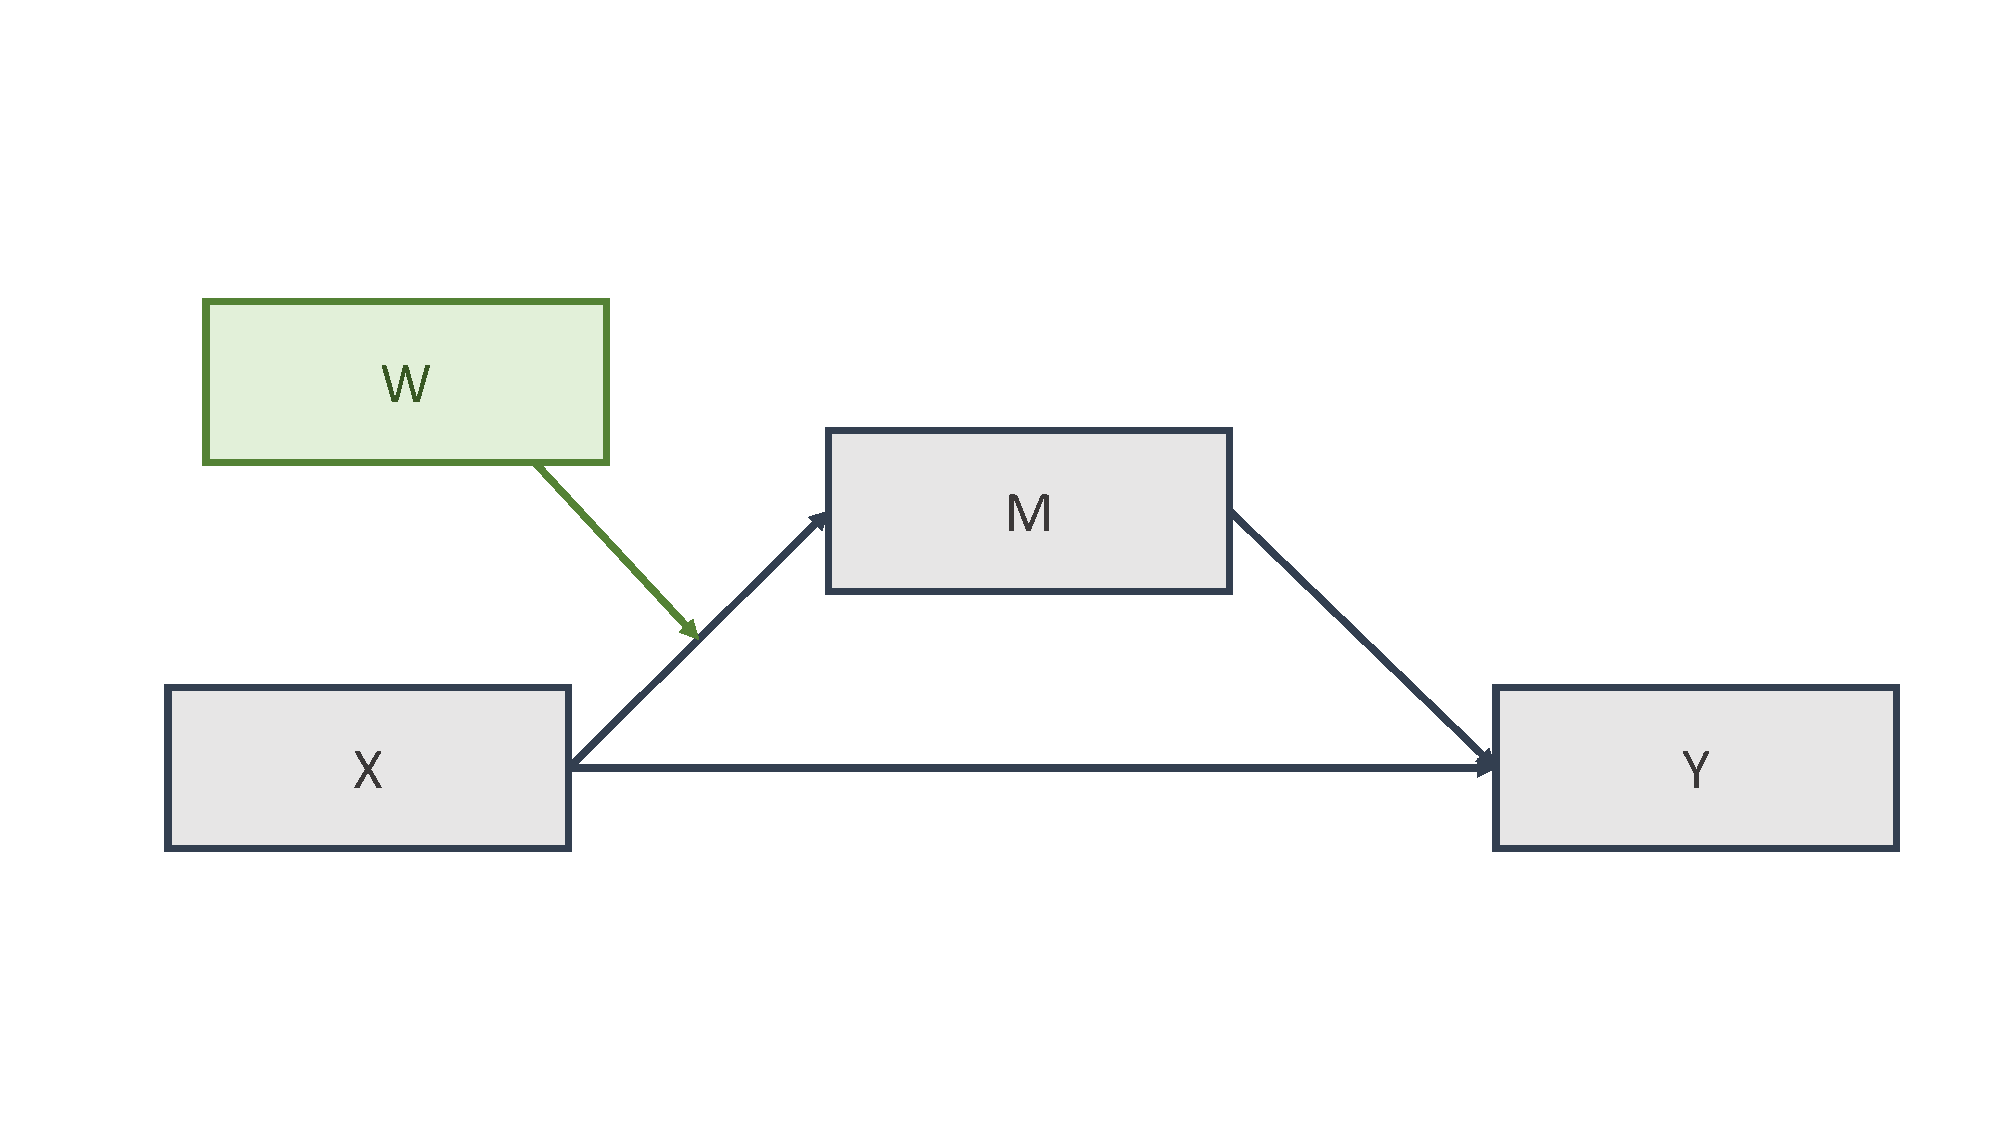
\includegraphics[width = \linewidth]{figures/fig_mod_med.pdf}
\caption{An example of moderated mediation, where the moderator (denoted W), moderates the effect of X on M (the a path).}
\label{fig:modmed}
\end{figure}

In general, interactions make interpretation more difficult. In linear
models, the interpretation of the interaction estimate becomes: ``a one
unit increase in X is associated with a
\(\beta_x + \beta_{int} \times W\) effect on the outcome.'' That is, to
understand the size, and direction, of the effect of X, the level of W
must be considered. For example, if W is a categorical variable with
values of 0 and 1, and the following regression was estimated:

\begin{equation}
\hat{M}_i = 1.0 + 5.0 X + 3.0 W + .5 X*W
\end{equation}

\noindent then:

\begin{enumerate}
\def\labelenumi{\arabic{enumi}.}
\tightlist
\item
  X is associated with a 5.0 increase in M when W is 0, and
\item
  X is associated with a 5.5 increase in M when W is 1.
\end{enumerate}

\noindent The same logic holds for continuous moderators, although
representative values of W must be chosen instead of using all possible
values.

Yet, in non-linear situations, this becomes more strenuous. However,
using average marginal effects, the interpretation can be like that of
linear models. In general, this has been done by selecting various,
representative values of W at which the average marginal effect is
assessed (StataCorp, 2015). If W is categorical then all observed values
can be used. Notably, in linear and generalized linear models,
moderation is probably best understood using visualizations---showing
the effect of X at various levels of W (see Figure
\ref{fig:interaction}).

\begin{figure}[tb]
\centering
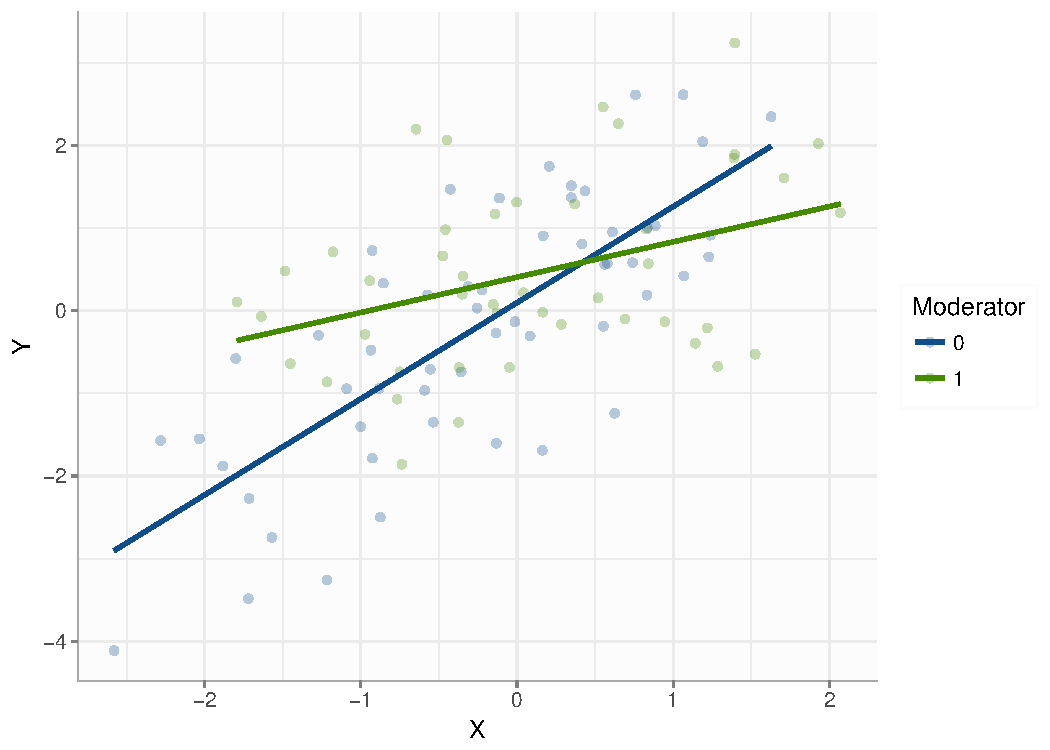
\includegraphics[width = \linewidth]{figures/fig_interaction_effect.pdf}
\caption{An example of a common approach to visualizing a moderation effect where the effect of X on Y is shown for each level of W.}
\label{fig:interaction}
\end{figure}

In relation to MMA, moderation can be understood at both 1) an
individual path level and 2) a complete model level. At an individual
path level, moderation is understood as it is in non-mediating
regression situations. For example, if path a is moderated, the effect
of X on M can be understood via visualizations or representative values
of W can be inserted into the regression equation, as in the example
above.

To understand it in relation to the complete model, the framework
discussed by Edwards and Lambert (2007) suggests using the \emph{reduced
form} of the mediation model to understand the moderation in the context
of the indirect and direct effects. The reduced form refers to having
only exogenous variables on the right-hand side of the equation (i.e.,
substituting the estimates of the a path into the b/c path model) as
shown below.

Starting with the non-reduced form, we have \(M_i\), an endogenous
variable, on the right hand side.

\begin{equation}
Y_i = \beta_0 + b_1 M_i + c^{`}_1 x_i + \epsilon_{yi}
\end{equation}

\noindent Using the a path model, and assuming the same model
specification as in Figure \ref{fig:modmed}, we can substitute in the
predictors of \(M_i\).

\begin{equation}
Y_i = \beta_0 + b_1 (a_0 + a_1 x_i + a_2 w_i + a_3 x_i * w_i) + c^{'}_1 x_i + \epsilon_{yi}
\end{equation}

\noindent This form is now reduced so that only exogenous variables are
on the right-hand side. Using these estimates, it is now possible to
assess the effect of \(x\) on \(Y\) when it depends on the level of
\(w\) using the same approach with the individual paths. Importantly,
using these estimates, the moderated effect of \(x\) can be visualized
as well.

\subsection{The Decomposed Total Effect Equals The Total
Effect}\label{the-decomposed-total-effect-equals-the-total-effect}

When using the average marginal effect, the decomposed total effect
(\(a \times b + c'\)) equals that of the original total effect (\(c\)).
Winship and Mare (1983), demonstrated that, using calculus, an outcome
variable Y can be decomposed by its total differential

\begin{equation}
dY = \frac{\delta Y}{\delta X}dX + \frac{\delta Y}{\delta M}dM
\end{equation}

\noindent which implies the general formula

\begin{equation}
\frac{dY}{dX} = \frac{\delta Y}{\delta X} + \frac{\delta Y}{\delta M}\frac{dM}{dX}
\end{equation}

\noindent (pg. 83, the symbols were altered to match that of the present
project). That is, the total effect is equal to the direct plus indirect
effects. If the average marginal effect is a good estimate of the
derivative (or partial derivative), then:

\begin{equation}
\frac{dY}{dX} = \frac{\delta Y}{\delta X} + \frac{\delta Y}{\delta M}\frac{dM}{dX} = c' + b \times a = c
\end{equation}

\noindent Therefore, it is expected that regardless of the distributions
of the mediators or outcomes \(a \times b + c' = c\).

This is further demonstrated with finite sampling properties in the
Monte Carlo simulation in Phase II using both binary and count
mediators.

\section{Standardized Effects}\label{standardized-effects}

It is often of considerable worth to understand standardized effects.
These can be defined in numerous ways, depending on the situation and
types of variables that are being used. In situations where the outcome
is continuous, MMA can use a partial standardization approach discussed
by Preacher and Hayes (2011) where the outcome is standardized using its
own standard deviation. This produces interpretations that are based on
the change in the outcome in standard deviation units. If using a
dichotomous predictor, this essentially becomes a standardized mean
difference (e.g., Cohen's D). It is also possible to standardize both
the continuous outcomes and continuous predictors to obtain a partial
correlation metric from these models as well.

As discussed below, the software to perform MMA includes the outcome
standardization for continuous outcomes but does not provide
standardization techniques for the predictors. Future iterations of the
software will include this as
well.\footnote{The researcher can standardize the continuous predictors and outcomes before performing MMA, in which case they can obtain the partial correlation estimates with the current version of the software.}

\section{Software Development}\label{software-development-1}

The software package developed for MMA is called
\texttt{MarginalMediation} and is freely available via the R statistical
environment. The software allows straightforward use of MMA across
continuous, binary, and count mediators and/or outcomes (other
distributions also work but have not been extensively tested). The
computation is done in several steps:

\begin{enumerate}
\def\labelenumi{\arabic{enumi}.}
\tightlist
\item
  Function and model checks
\item
  \(a\) path average marginal effect estimates
\item
  \(b\) and \(c'\) path average marginal effect estimates
\item
  Bootstrapped confidence intervals
\item
  Formatting and printing of the output
\end{enumerate}

This strategy was undertaken to help in error-checking and allows the
function to print informative output to the user during the modeling,
which is especially useful for situations with large samples and many
bootstrapped samples.

\subsection{Functions}\label{functions}

Using the package is based on a single function---\texttt{mma()}---that
provides the main functionality (Figure \ref{fig:mma}). \texttt{mma()}
is built on several other functions that perform specific duties that
allow the simple syntax. The main functions of the package are shown in
Table \ref{tab_functions}.

\begin{figure}[tb]
\centering
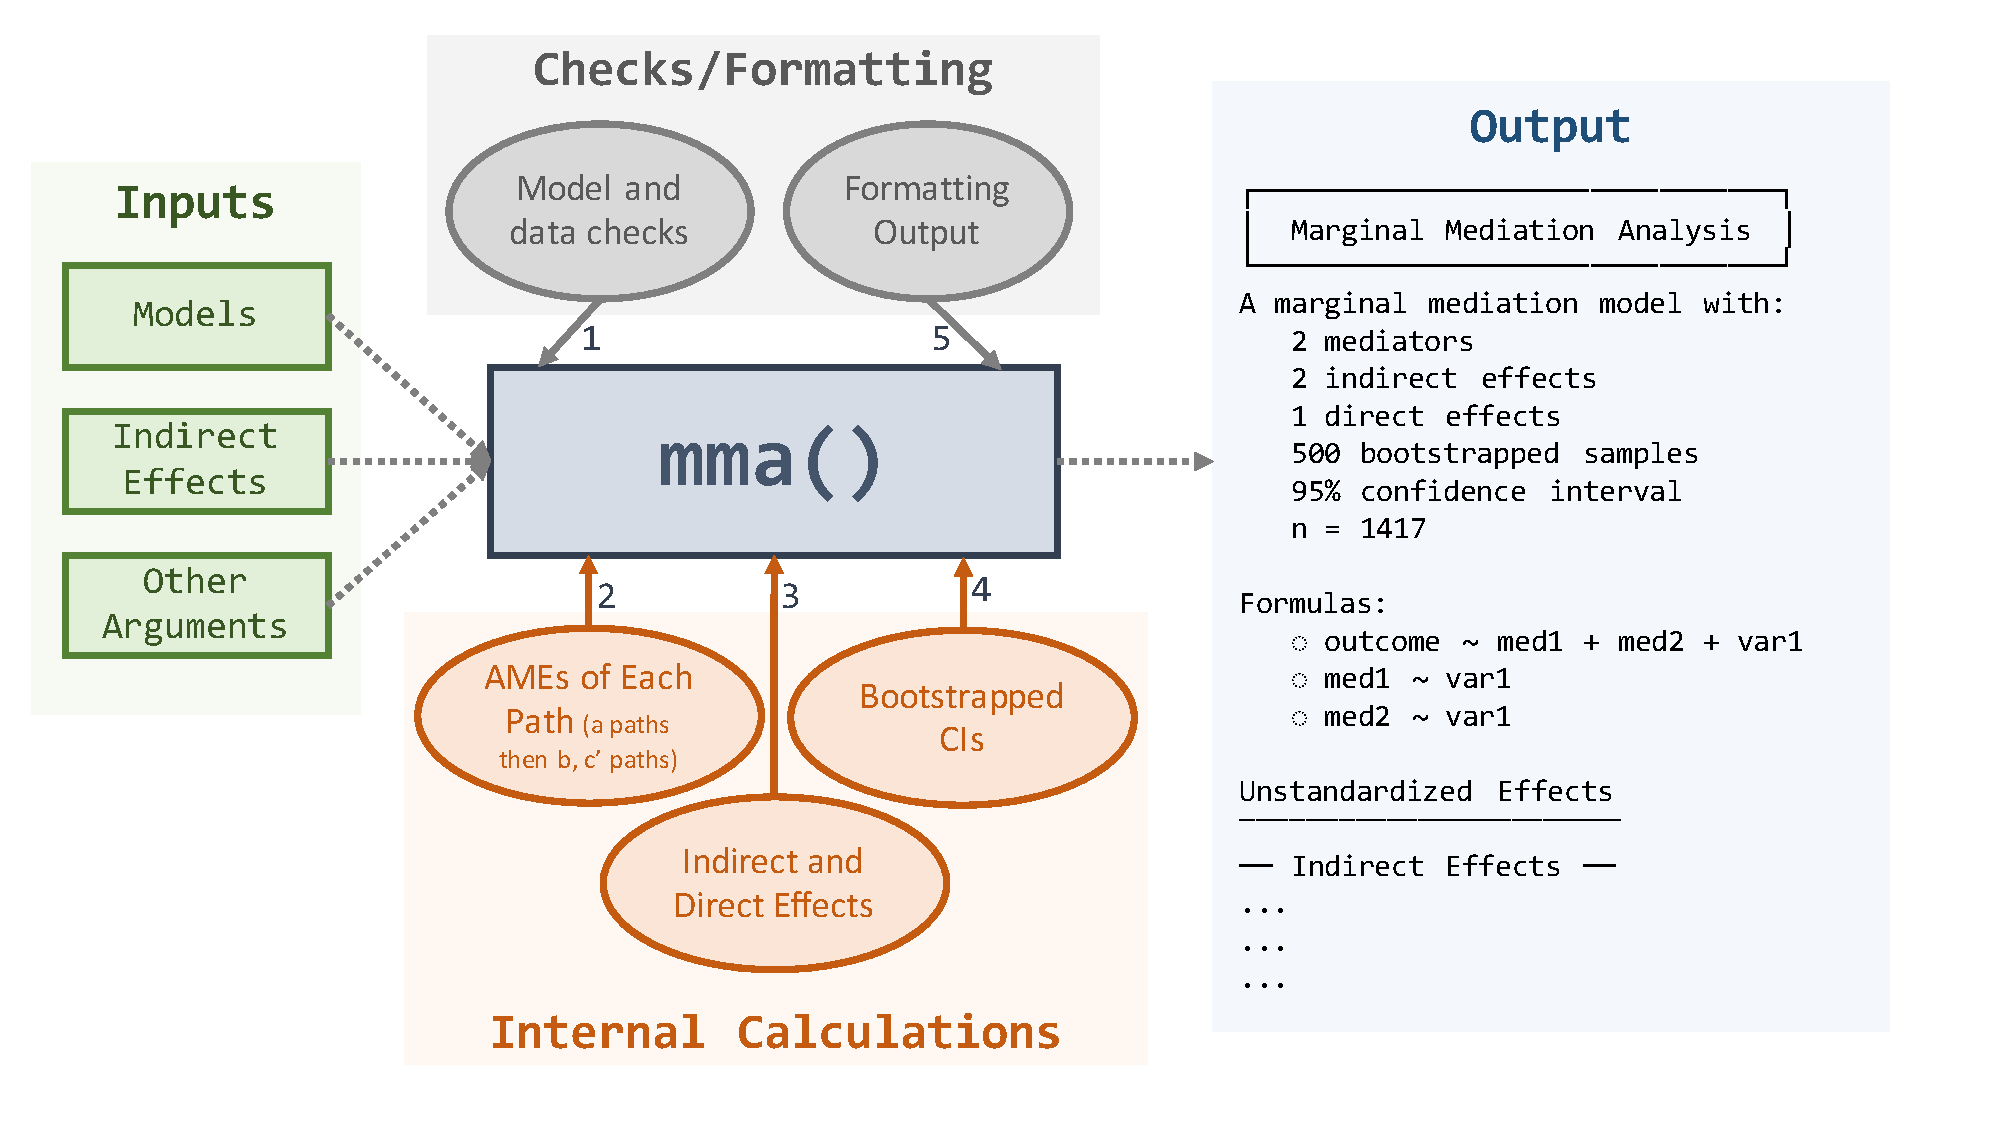
\includegraphics[width = \linewidth]{figures/fig_mma_structure.pdf}
\caption{The structure of the \texttt{mma()} function. From left to right: (1) inputs inform the function of the model specifications, the indirect effects to be reported, and other arguments; (2) internal processes including checks/formatting and internal calculations, (3) the output with some truncated example output. Notably, the numbers along the solid arrows pointing at the \texttt{mma()} function show the order of the operations, namely checks, AMEs, indirect and direct effects, bootstrapped confidence intervals, and formatting of the output.}
\label{fig:mma}
\end{figure}

\begin{table}[tb] 
\centering 
\caption{Functions used in the \texttt{MarginalMediation} R package.}
\label{tab_functions}
\begin{tabular}{p{38mm}p{45mm}p{55mm}}
\toprule
Type                & Function         & Behavior   \\ 
\midrule
Main Function            & \verb|mma()|     & Performs the full MMA model  \\
Marginal Function        & \verb|amed()|    & Computes the average marginal effects of a given GLM model   \\ 
Moderated Mediation      & \verb|mod_med()| & Computes the marginal effects at various levels of a moderator (still in testing) \\
Checks and formatting    & These functions perform behind the scenes & Check model specification and function requirements  \\ 
Other Functions          & \verb|mma_std_ind_effects()| and \verb|mma_std_dir_effects()| & Obtain the standardized indirect and direct effects from the model \\
Other Functions          & \verb|mma_ind_effects()| and \verb|mma_dir_effects()| & Obtain the unstandardized indirect and direct effects from the model \\
Other Functions          & \verb|perc_med()| & Obtain the percent of mediation for each specified path in the model \\
\bottomrule
\end{tabular}
\end{table}

\subsection{Computation of the Marginal
Effect}\label{computation-of-the-marginal-effect}

\texttt{MarginalMediation} uses built-in R functionality that allows for
relatively fast computation of the marginal effects. The approach taken
here is identical to that of the \texttt{margins} R package (Leeper,
2017), as described in Chapter 3. This is repeated here. Specifically,
for continuous predictors, the numerical derivative is used as shown
below where \(a\) is the general symbol for the model estimates.

\begin{equation}
AME_k = \frac{1}{n} \sum_{i = 1}^n \frac{f(aX_1) - f(aX_2)}{2h}
\end{equation}

\noindent where

\begin{equation}
aX_1 = \begin{bmatrix}
ax_{11} & ax_{12} & \dots & ax_{1k} + h & \dots & ax_{1p} \\
ax_{21} & ax_{22} & \dots & ax_{2k} + h & \dots & ax_{2p} \\
\vdots  & \vdots  & \ddots & \vdots     & \ddots  & \vdots \\
ax_{n1} & ax_{n2} & \dots & ax_{nk} + h & \dots & ax_{np}
\end{bmatrix}
\end{equation}

\noindent and

\begin{equation}
aX_2 = \begin{bmatrix}
ax_{11} & ax_{12} & \dots & ax_{1k} - h & \dots & ax_{1p} \\
ax_{21} & ax_{22} & \dots & ax_{2k} - h & \dots & ax_{2p} \\
\vdots  & \vdots  & \ddots & \vdots     & \ddots  & \vdots \\
ax_{n1} & ax_{n2} & \dots & ax_{nk} - h & \dots & ax_{np}
\end{bmatrix}
\end{equation}

\noindent With a small \(h\) (default is \(1 \times 10^{-7}\)), this
produces the average marginal effect across all the observations (e.g.,
the average change in the predicted value for a very small increase and
a very small decrease in in the \(x_k\) variable).

For discrete predictors, the discrete difference is used as shown below,

\begin{equation}
AME_{k} = \frac{1}{n} \sum_{i=1}^{n} \big[ F(\beta X | x_{ki} = 1) - F(\beta X | x_{ki} = 0) \big]
\end{equation}

\noindent where \(F(\beta X | x_{ki} = 1)\) is the predicted value of
the \(ith\) observation when the dummy variable \(x_k\) equals one and
\(F(\beta X | x_{ki} = 0)\) is the predicted value when the dummy value
of \(x_k\) equals zero holding all other variables constant. This, in
effect, shows the discrete difference between the levels of the
categorical variable in the outcome's original units.

These approaches are employed in \texttt{MarginalMediation} due to their
flexibility across GLM types and model specifications. For example, it
can handle many types of models (e.g., linear, GLM, multilevel) and can
produce more interpretable estimates of the marginal effects of
predictors that have quadratic terms (e.g., \(age\) and \(age^2\)).

\subsubsection{Standardization}\label{standardization}

As was briefly noted earlier, partial standardization wherein the
outcome is standardized is possible when the outcome is continuous. In
these situations, the output of \texttt{MarginalMediation} will include
both unstandardized and standardized effects (see Figure
\ref{fig_mmaexample}).

\subsection{Examples of Software Use}\label{examples-of-software-use}

To briefly demonstrate the use of \texttt{mma()}, fictitious data were
first generated, where X, M, and Y are continuous. Using these data
(called \texttt{df1}), the following \texttt{R} code demonstrates the
use of \texttt{mma()} in the simplest case.

\singlespacing

\begin{Shaded}
\begin{Highlighting}[]
\KeywordTok{library}\NormalTok{(MarginalMediation)}

\NormalTok{pathbc =}\StringTok{ }\KeywordTok{glm}\NormalTok{(Y }\OperatorTok{~}\StringTok{ }\NormalTok{X }\OperatorTok{+}\StringTok{ }\NormalTok{M, }\DataTypeTok{data =}\NormalTok{ df1)}
\NormalTok{patha  =}\StringTok{ }\KeywordTok{glm}\NormalTok{(M }\OperatorTok{~}\StringTok{ }\NormalTok{X, }\DataTypeTok{data =}\NormalTok{ df1)}

\NormalTok{fit =}\StringTok{ }\KeywordTok{mma}\NormalTok{(pathbc,}
\NormalTok{          patha,}
          \DataTypeTok{ind_effects =} \KeywordTok{c}\NormalTok{(}\StringTok{"X-M"}\NormalTok{))}
\end{Highlighting}
\end{Shaded}

\doublespacing

First, the individual sub-models are fit thereby creating
\texttt{pathbc} and \texttt{patha} which are both \texttt{glm} objects.
Then, the b and c paths (\texttt{pathbc}) model object is the first
argument to \texttt{mma()}, followed by the a paths (in this case only a
single a path but multiple---separated by commas---can be included). The
necessary argument is the \texttt{ind\_effects}. This argument expects a
vector or list of quoted paths, where the paths are the form
\texttt{"predictor-mediator"}. In this case, the predictor is called
\texttt{X} and the mediator is called \texttt{M}.

The \texttt{fit} object as created by \texttt{mma()} contains a number
of elements, including the indirect effects, the direct effects, the
confidence interval, and the original data. Figure \ref{fig_mmaexample}
provides an example of how the output could look if the \texttt{fit}
object is printed. This output provides both unstandardized effects
(both indirect and direct) that are in the units of the outcome and
standardized effects---using the standard deviation of the outcome as
recommended by MacKinnon (2008)---which are in the standard deviation
units of the outcome.

\begin{figure}[tb]
\centering
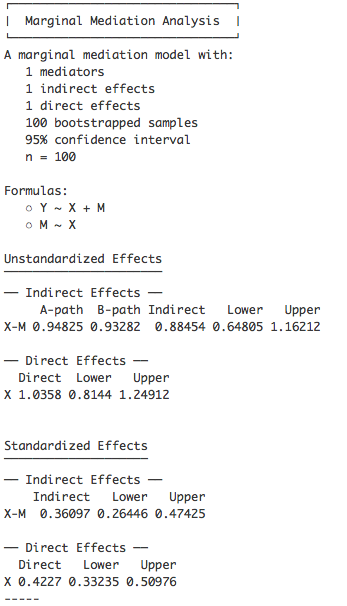
\includegraphics[width = 0.5\textwidth]{figures/fig_mma_example.png}
\caption{An example of the output from the \texttt{mma()} function.}
\label{fig_mmaexample}
\end{figure}

Further, it can be assessed whether, in this case, the indirect plus the
direct effects equal the total effect. Here, the total effect is 1.921
which is equal to the indirect effect (0.885) plus the direct effect
(1.036). This suggests that comparisons between the effects can be
confidently made.

If a covariate, \(X2\) is added to the data, this can be easily added to
the model as shown below.

\singlespacing

\begin{Shaded}
\begin{Highlighting}[]
\KeywordTok{library}\NormalTok{(MarginalMediation)}
\NormalTok{pathbc =}\StringTok{ }\KeywordTok{glm}\NormalTok{(Y }\OperatorTok{~}\StringTok{ }\NormalTok{X }\OperatorTok{+}\StringTok{ }\NormalTok{X2 }\OperatorTok{+}\StringTok{ }\NormalTok{M, }\DataTypeTok{data =}\NormalTok{ df1)}
\NormalTok{patha  =}\StringTok{ }\KeywordTok{glm}\NormalTok{(M }\OperatorTok{~}\StringTok{ }\NormalTok{X }\OperatorTok{+}\StringTok{ }\NormalTok{X2, }\DataTypeTok{data =}\NormalTok{ df1)}

\NormalTok{fit2 =}\StringTok{ }\KeywordTok{mma}\NormalTok{(pathbc,}
\NormalTok{           patha,}
           \DataTypeTok{ind_effects =} \KeywordTok{c}\NormalTok{(}\StringTok{"X-M"}\NormalTok{,}
                           \StringTok{"X2-M"}\NormalTok{))}
\end{Highlighting}
\end{Shaded}

\doublespacing

It is also possible to access various aspects of these MMA model fit
objects.

\begin{Shaded}
\begin{Highlighting}[]
\KeywordTok{perc_med}\NormalTok{(fit2, }\StringTok{"X-M"}\NormalTok{)}
\end{Highlighting}
\end{Shaded}

\noindent This informs the researcher that the indirect effect accounts
for approximately 44\% of the total effect from X to Y in \texttt{fit2}.

\section{Monte Carlo Simulation
Study}\label{monte-carlo-simulation-study}

With the software package \texttt{MarginalMediation}, the simulations
were able to assess the package's functionality and the overall
framework's ability to estimate the underlying effects accurately.
First, to assess the appropriateness of the experimental conditions, a
literature review was conducted.

\subsection{Literature Review}\label{literature-review-1}

Studies were sought that saliently reported results wherein both
mediation analysis and generalized linear models were used. Since 2012,
this produced 57 articles (via
Scopus).\footnote{The search terms included: "mediation analysis" and ["logistic" or "generalized linear models" or "GLM" or "poisson"].}
Among these, three general categories of articles were found:

\begin{enumerate}
\def\labelenumi{\arabic{enumi}.}
\tightlist
\item
  Articles that were methodologically building on mediation analysis.
\item
  Articles that applied mediation where a mediator and/or outcome was
  categorical and the authors used the ``difference method'' (MacKinnon,
  2008) to assess the amount of mediation.
\item
  Articles that applied mediation where a mediator and/or outcome was
  categorical and the authors either used the structural equation
  modeling approach or did not include the categorical mediator and/or
  outcome in the mediation.
\end{enumerate}

Of these, number two was most prevalent. The literature suggested that
the parameters selected for the simulations were relevant, particularly
the small effect sizes and large sample sizes. Most studies used extant,
large questionnaire data sets and the majority were cross-sectional.

Importantly, this search demonstrated the commonality of the
``difference method'' as discussed by MacKinnon (2008). This method
relies on the following:

\singlespacing

\begin{equation}
a \times b + c' = c
\end{equation}\begin{equation}
a \times b = c - c'
\end{equation}

\doublespacing

\noindent In essence, this says that it is possible to estimate the
indirect effect, that is \(a \times b\) by assessing the difference
\(c - c'\). However, in situations where the decomposed total effect
does not equal the total effect, this method may not be valid although
many studies still used this approach in categorical data situations.

\subsection{Simulations}\label{simulations-1}

The Monte Carlo simulation produced 45,000 marginal mediation models
(although including the bootstrapped intervals there were 22.5 million
models run). These simulated models were run on powerful Core i7
computers over the span of several days. The following subsections
discuss the results of the simulations in regard to each outcome of
interest.

\subsubsection{Decomposed Total Effect Equals The Total
Effect}\label{decomposed-total-effect-equals-the-total-effect}

One of the major questions about the performance of MMA regards whether
the decomposed total effect equals the total effect
(\(a \times b + c' = c\)). Table \ref{tab_discrep} highlights the
average discrepancy between the decomposed total effect and the total
effect divided by the total effect (thereby adjusting the discrepancy
for the size of the total effect). Clearly, on an average level,
deviations are extremely small, generally \textless{} .5\% discrepancy,
with the majority \textless{} .1\% discrepancy. The discrepancies also
decrease in size as the sample size increases.

\begin{table}[ht]
\centering
\caption{Average discrepancies between the decomposed total effect and the total effect for various sample sizes.}
\begin{tabular}{lcc}
\toprule
  & \multicolumn{2}{c}{Mediator} \\
Sample Size & Binary & Count \\ 
\midrule
  50   & 0.0017  & -0.0080 \\ 
  100  & 0.0024  & -0.0028 \\ 
  200  & 0.0007  &  0.0027 \\ 
  500  & 0.0001  & -0.0036 \\ 
  1000 & -0.0000 & -0.0027 \\ 
\bottomrule
\end{tabular}\label{tab_discrep}
\end{table}

Figure \ref{fig:totaltotal} presents the individual simulated
differences between the decomposed total effect and the total effect.
Once assessing the individual discrepancies, two patterns are of note:

\begin{enumerate}
\def\labelenumi{\arabic{enumi}.}
\tightlist
\item
  There are larger discrepancies for smaller sample sizes and larger
  effect sizes.
\item
  Besides a single outlier in the count condition (Panel b), most
  discrepancies are small.
\end{enumerate}

First, the largest discrepancies are where the sample sizes are small (n
= 50) and the effect sizes are larger. This is intuitive in that as the
effect size is larger, the amount of discrepancy that is still
considered small also increases (i.e., variability simply due to the
estimates being on a larger scale). For both binary and count mediators,
the discrepancies, even in the large effect sizes, are very small as the
sample increases to n = 1000. Given the literature review, this is a
sample size that is often possible in the health and prevention
sciences. Further, most effect sizes in the literature were moderate or
smaller. These conditions had low variability in the discrepancy.

Second, in the count condition there is a clear outlying value
(\textgreater{}2 for the n = 50 and large/large effect size condition).
Other than this value---across the binary and count mediators---all
other values are relatively close to zero. For the binary mediator
condition, the scale was in risk (probability) units. The discrepancies,
here, in the n = 50 condition are notable in their size while the other
conditions had discrepancies that are essentially within rounding error.
For the count mediator condition, the scale of the total effect was in
count units. The outlier is notable in its large discrepancy in these
units; most other values were essentially within rounding error of the
effect size.

\begin{figure}[tb]
\centering
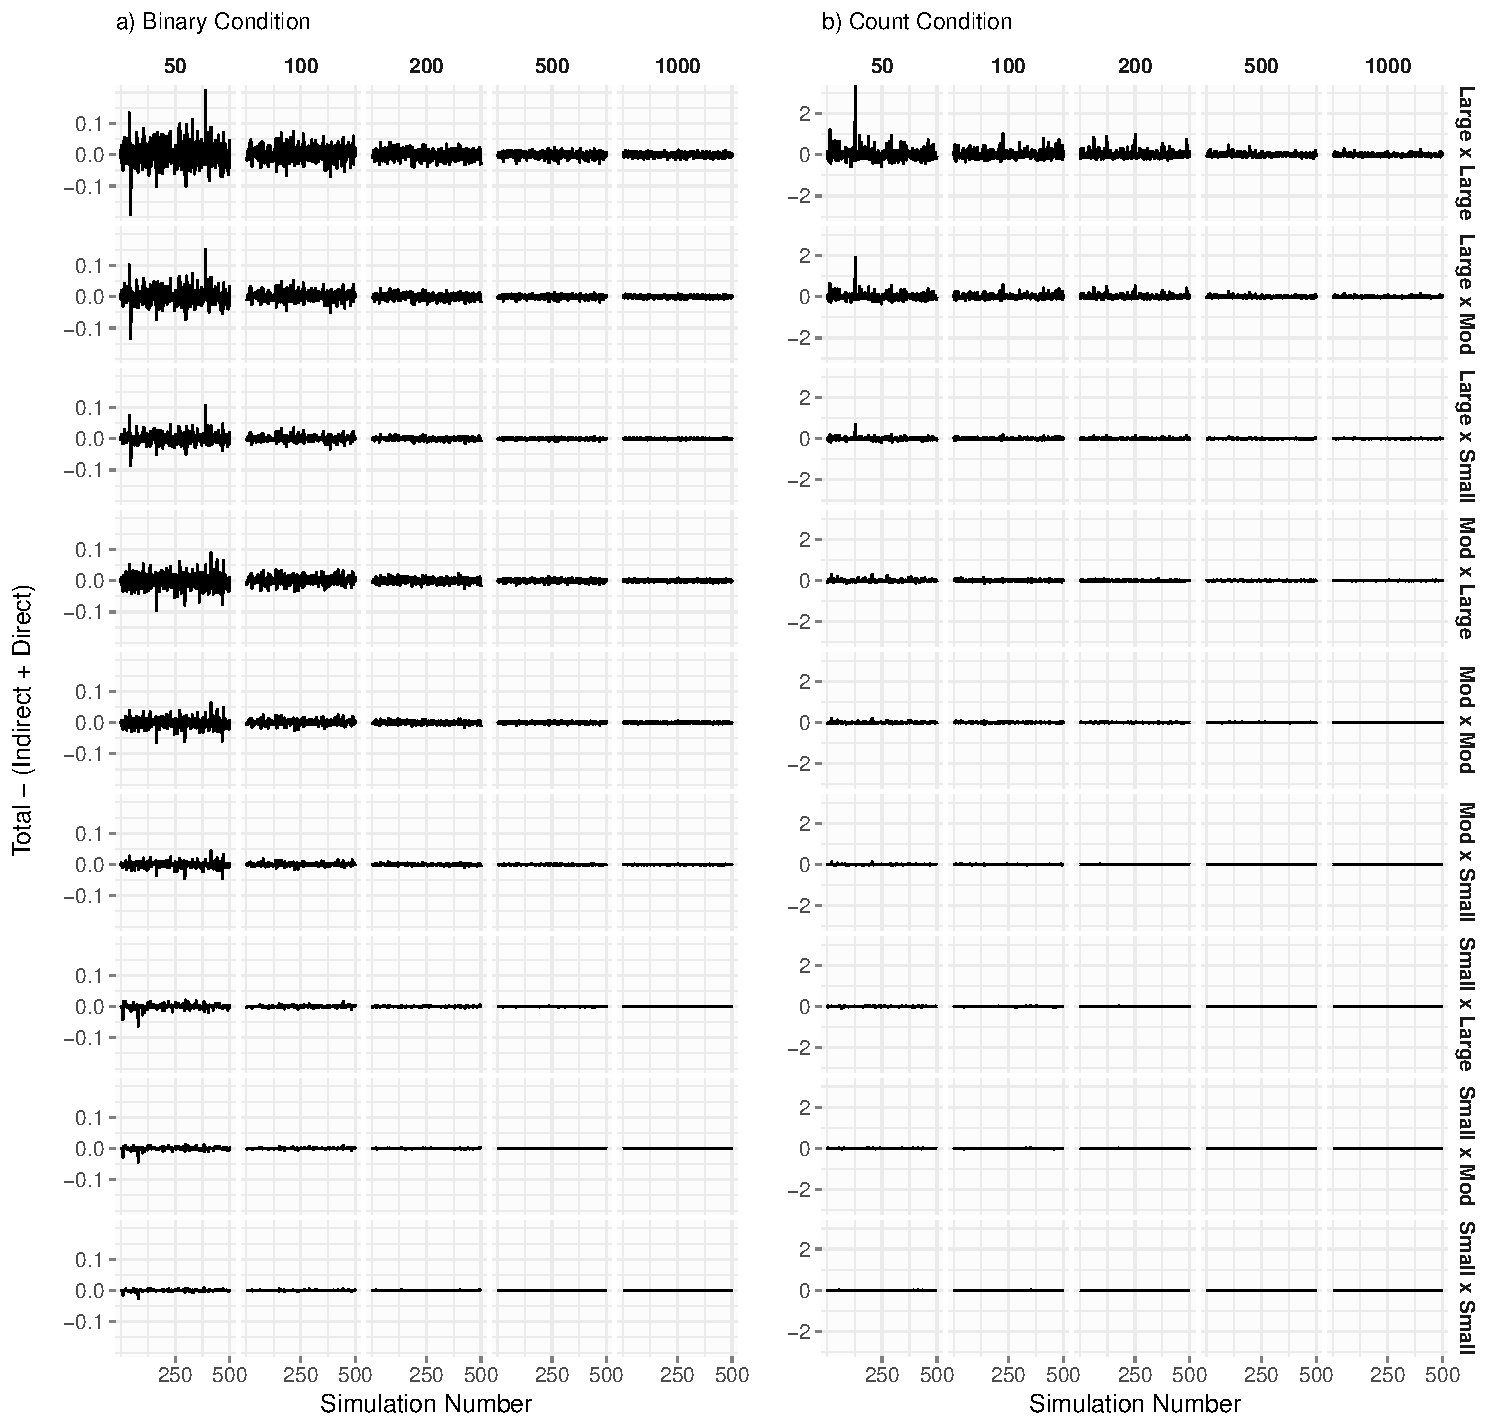
\includegraphics[width = \linewidth]{figures/fig_total_total.pdf}
\caption{The simulated differences between the decomposed total effect and the total effect. The discrepancies are higher for smaller sample sizes and larger effect sizes.}
\label{fig:totaltotal}
\end{figure}

Ultimately, this provides evidence of MMAs ability to estimate values
that let the \(a \times b + c' = c\) condition to hold, even in
individual applications. This, however, is somewhat dependent on the
sample size. As for differences across the effect sizes of the a and b
paths, as an effect size increases so does the level of ``rounding
error.'' That is, in large effects, larger discrepancies are still a
minor deviation than if the effect was small. Therefore, the main aspect
of this finding is that sample size is important in the accuracy of the
indirect plus direct equaling the total effect.

\subsubsection{Statistical Power}\label{statistical-power}

Figure \ref{fig_power} shows the statistical power of MMA across the
various conditions. The figure shows the statistical power at each
tested sample size for each combination of effect sizes (e.g., ``Mod x
Large'' is a moderate a path effect size and a large b path effect
size). Overall, most effect size combinations are adequately powered at
a sample size of 200 across both binary and count mediator conditions.
Interestingly, the ``Small x Small'' condition had more power at higher
sample sizes than ``Large x Small'', which is contrary to intuition.
However, the issue here was the issue of \emph{complete separability}
wherein the estimates and the standard errors are either biased or not
estimable in logistic regression. With a large effect and a large sample
size, this became common, thus reducing the statistical power in these
conditions. The count mediator condition did not have this issue.

\begin{figure}[tb]
\centering
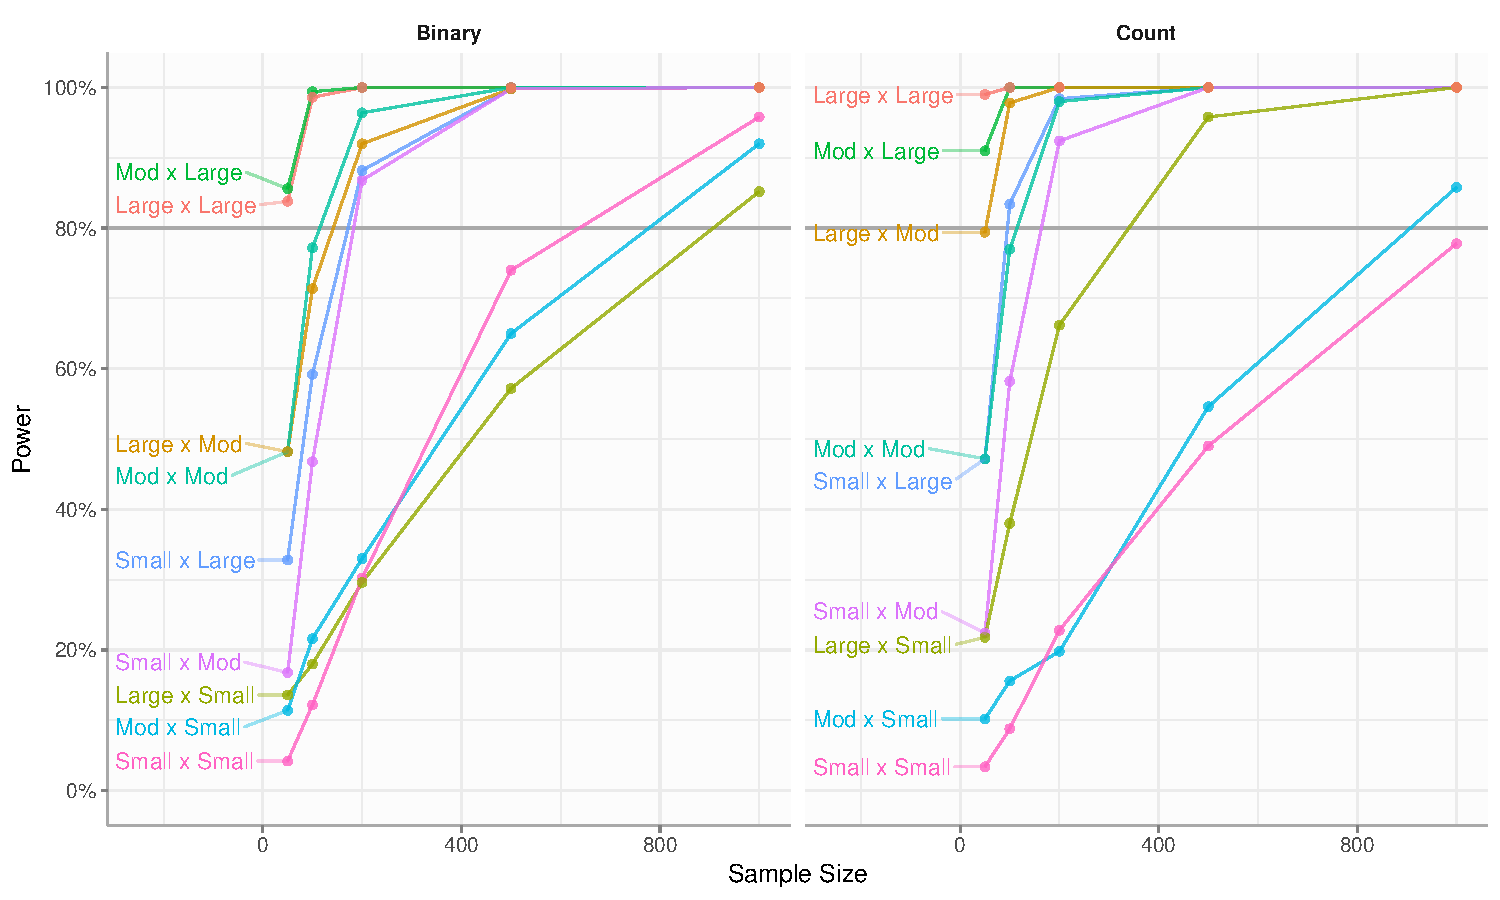
\includegraphics[width = \linewidth]{figures/sim_fig_power.pdf}
\caption{The simulated levels of power per tested sample size (x-axis) and effect size of the indirect path (color; a combination of the a path by the b path) stratified by the distribution of the mediator (binary or count).}
\label{fig_power}
\end{figure}

Overall, the method has the statistical power for even very small
indirect effects with a sample size of 1000. As mentioned before, sample
sizes greater than 1000 are common in the literature suggesting the
method can be used even to detect small effect sizes.

\subsubsection{Estimation Accuracy}\label{estimation-accuracy}

It is also important for MMA to estimate the expected parameters. Figure
\ref{fig_acc} highlights that MMA is consistent in estimating the
underlying effects for each combination of effect sizes across the
various sample sizes. In the figure, which is stratified by the
combination of effect sizes, shows the population parameter (vertical
lines) and the estimated values (the density distributions). Overall,
the distributions are centered at the true population parameter in each
situation across the conditions.

\begin{figure}[tb]
\centering
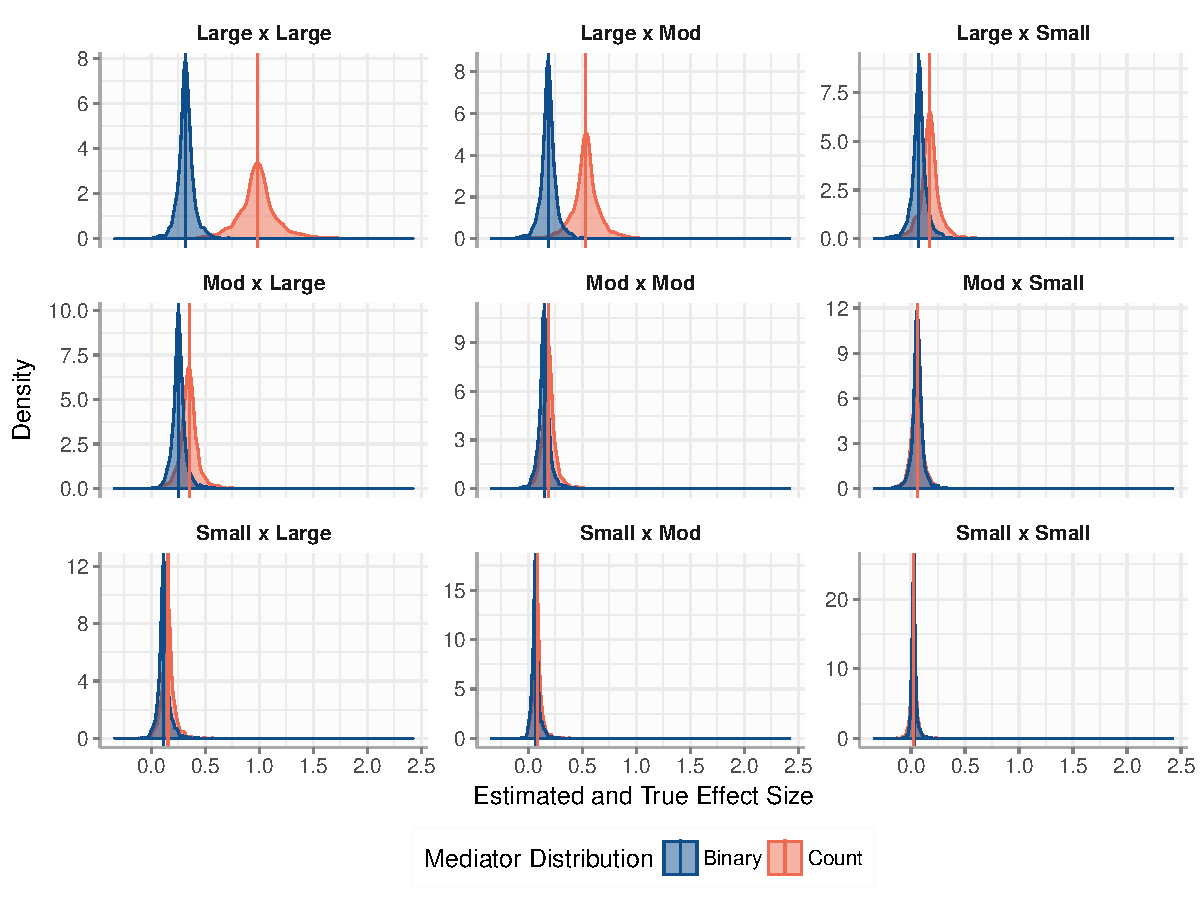
\includegraphics[width = \linewidth]{figures/sim_fig_acc.pdf}
\caption{The simulated accuracy per tested sample size (x-axis) and effect size of the indirect path (color; a combination of the a path by the b path).}
\label{fig_acc}
\end{figure}

As also seen in Figure \ref{fig:totaltotal}, there is more variability
in the estimation for larger effect sizes than for smaller. Again, this
variability is likely due to the estimates being on a larger scale.

\subsubsection{Confidence Interval
Coverage}\label{confidence-interval-coverage}

Finally, the confidence interval coverage is shown in Figure
\ref{fig_ci}. Panel a) of the figure shows the overview---that the
confidence interval coverage is around the 95\% line for both the binary
and count mediator conditions. However, looking at it much more closely
in Panel b) it is clear that there is some deviation from the 95\% line,
particularly in the binary mediator condition. This is not a major
deviation but an important one, nonetheless. Given the use of the
percentile bootstrapping method herein, it may be important to apply
other bootstrapping approaches such as the Bias-Corrected Bootstrap.

\begin{figure}[tb]
\centering
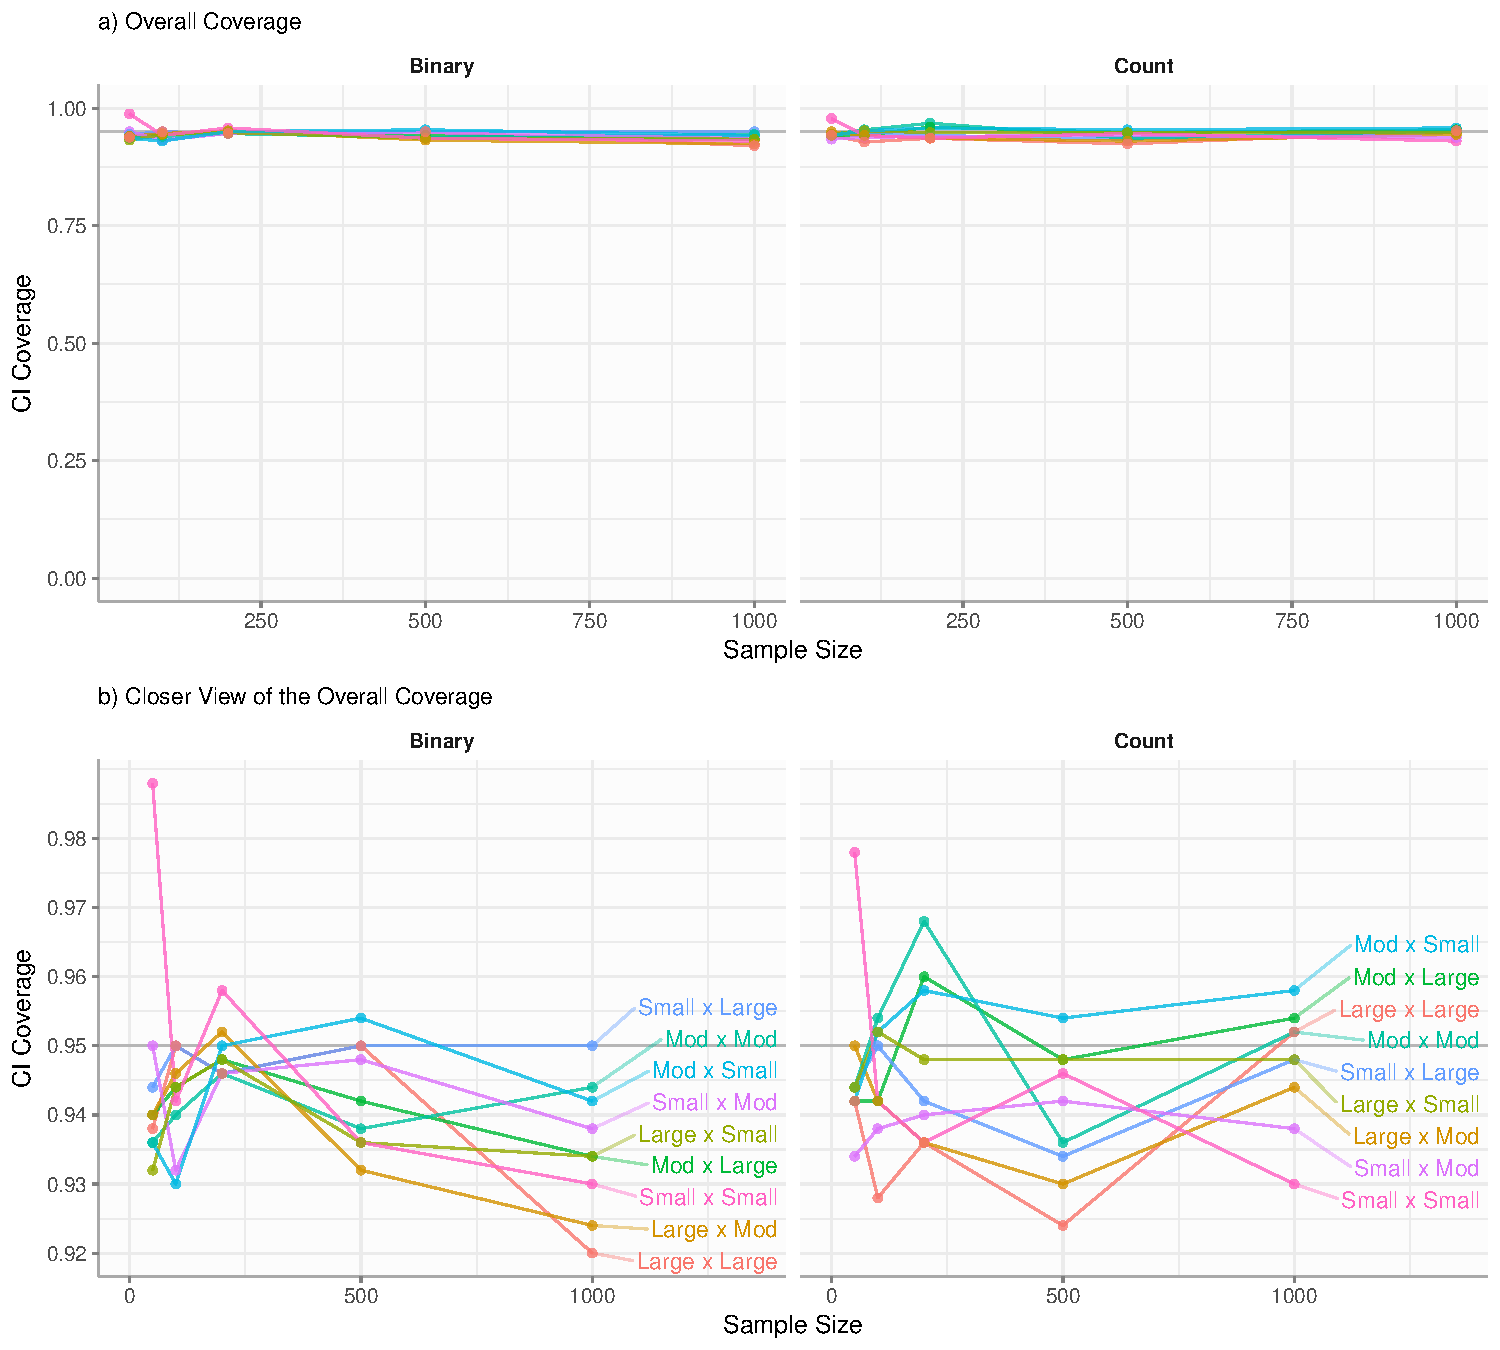
\includegraphics[width = \linewidth]{figures/sim_fig_ci.pdf}
\caption{The simulated confidence interval coverage per tested sample size (x-axis) and effect size of the indirect effect . The "ideal" level is set at 0.95. Panel a) shows that the confidence intervals from a broad perspective. Panel b) provides a closer look at the individual patterns of the confidence intervals around the ideal level of 0.95.}
\label{fig_ci}
\end{figure}

This finding of the indirect effect having confidence intervals that
were too narrow has been found previously for the percentile
bootstrapped (as applied in MMA; MacKinnon, Lockwood, and Williams,
2004). However, MacKinnon et al. (2004) also found the bootstrap
methods, including the percentile approach, is among the best of the
tested approaches. Other approaches, including the Monte Carlo
confidence interval can be tested in future studies.

\section{Conclusion}\label{conclusion}

Marginal Mediation Analysis shows promise in its ability to accurately
estimate models wherein the mediator is a binary or a count variable.
Results regarding the decomposed total effect equaling the total effect
are positive, although the estimation accuracy of this relationship
depends on the sample and effect sizes. The statistical power is
comparable to other modern mediation techniques wherein even small
effect sizes can be estimated with a sample size of 1000. The estimation
is consistent, ultimately averaging at the true population value. The
confidence interval coverage was often too narrow for the binary
mediator condition---sometimes having coverage of just above 92\%---but
it was approximately correct for the count mediator condition with some
variability around 95\%. Finally, the software for MMA is free to use in
the R statistical environment in the \texttt{MarginalMediation} package.
This allows researchers to begin to use the approach with little
overhead. All in all, MMA appears to be a practical approach to
difficult mediation situations.

\singlespacing

\FloatBarrier

\newpage

\fancyhead[L]{Phase III} \fancyhead[R]{\thepage} \fancyfoot[C]{}

\chapter{PHASE III: APPLICATION OF MMA}

\begin{quote}
\emph{The power of intuitive understanding will protect you from harm until the end of your days.}
--- Lao Tzu
\end{quote}

\doublespacing

\section{Introduction}\label{introduction-5}

In 2012, Ford and Hill published an article that used some of the most
common approaches to mediation when a mediator and/or outcome is
categorical. Specifically, they used:

\begin{enumerate}
\def\labelenumi{\arabic{enumi}.}
\tightlist
\item
  the difference method (MacKinnon, 2008),
\item
  the ``categorical data method outlined by MacKinnon (2008)'' (pg. 5)
  to assess the significance of the difference method, and
\item
  the percent of the total effect that was mediated.
\end{enumerate}

These three approaches are not only common but likely some of the best
approaches in this situation. However, as stated in Chapter 4, these
have some notable shortcomings. First, the standard errors can be
inefficient and biased if there is a high degree of multi-collinearity
(or the degree to which there is perfect separability) in any of the
models.\footnote{Perfect separability is where a predictor can perfectly predict the outcome in logistic regression.}
The significance of the difference method depends on these standard
error estimates. Second, it does not provide the effect size measures
that would be most useful {[}e.g., the effect of increasing the
predictor on the outcome through the mediator(s){]}. Third, the
difference method is consistently too conservative with binary outcomes
(Jiang and Vanderweele, 2015).

To build on the important findings from Ford and Hill (2012), this study
replicates their work using more recent data from 2014 while using MMA
to obtain effect sizes and confidence intervals for the indirect and
direct effects.

\section{Results}\label{results}

\begin{verbatim}
## Error in eval(expr, envir, enclos): object 'da36361.0001' not found
\end{verbatim}

\begin{verbatim}
## Error in tolower(names(d)): object 'd' not found
\end{verbatim}

\begin{verbatim}
## Error in eval(lhs, parent, parent): object 'd' not found
\end{verbatim}

\begin{verbatim}
## Error in map(.x, .f, ...): object 'd1' not found
\end{verbatim}

\begin{verbatim}
## Error in map_lgl(.x, .p, ...): object 'd1' not found
\end{verbatim}

\begin{verbatim}
## Error in eval(lhs, parent, parent): object 'd1' not found
\end{verbatim}

\begin{verbatim}
## Error in library(here): there is no package called 'here'
\end{verbatim}

\begin{verbatim}
## Error in here("Data/NSDUH_2014_Results.rda"): could not find function "here"
\end{verbatim}

\begin{verbatim}
## Error in library(survey): there is no package called 'survey'
\end{verbatim}

\begin{verbatim}
## Error in svydesign(ids = ~1, strata = ~vestr, weights = ~analwt_c, data = d1): could not find function "svydesign"
\end{verbatim}

\begin{verbatim}
## Error in svyglm(self ~ religious + age2 + irsex + newrace2 + irfamin3 + : could not find function "svyglm"
\end{verbatim}

\begin{verbatim}
## Error in svyglm(peer ~ religious + age2 + irsex + newrace2 + irfamin3 + : could not find function "svyglm"
\end{verbatim}

\begin{verbatim}
## Error in svyglm(dep ~ religious + age2 + irsex + newrace2 + irfamin3 + : could not find function "svyglm"
\end{verbatim}

\begin{verbatim}
## Error in coef(obj): object 'svy_a1' not found
\end{verbatim}

\begin{verbatim}
## Error in rownames(est1) = c("Respondent", "Peer", "Depression"): object 'est1' not found
\end{verbatim}

\begin{verbatim}
## Error in data.frame(est1): object 'est1' not found
\end{verbatim}

\begin{verbatim}
## Error in svyglm(model, design = design, family = "quasibinomial"): could not find function "svyglm"
\end{verbatim}

\begin{verbatim}
## Error in UseMethod("vcov"): no applicable method for 'vcov' applied to an object of class "NULL"
\end{verbatim}

\begin{verbatim}
## Error in rownames(est2) = c("Tobacco", "Rx", "Marijuana", "Illicit"): object 'est2' not found
\end{verbatim}

\begin{verbatim}
## Error in data.frame(est2): object 'est2' not found
\end{verbatim}

The descriptive statistics are found in Table \ref{tab:table1} for the
13,600 adolescents in the sample. Overall, these sample statistics were
very similar to the 2007 sample used by Ford and Hill. However, the
prevalence of drug use across each category dropped since 2007, although
marijuana use did not drop substantially (13.85\% in 2007 to 12.7\% in
2014). Heavy drinking (10.4\% in 2007) had only a single positive
response in the entire sample of adolescents in 2014. Unfortunately, the
number of major depressive episodes increased from 8.4\% in 2007 to
11.3\% in 2014. Attitudes regarding drug use were essentially identical
as that in 2007 for the respondent, peer, and parent (and each had high
reliabilities---all \(\alpha \geq .80\)---comparable to 2007). Finally,
the attitudinal measures and the measure of religiosity had high
reliabilities.

\begin{table}[ htb ] 
\centering 
\caption{Descriptive statistics of the sample.}
\begin{tabular}{ lc }
\toprule
  & Mean/ Percent (SD) \\ 
  & n = 13,600 \\ 
\midrule
Drug use & \\
\hspace{6pt} Prescription drug misuse (past year) & 5.7\% \\ 
\hspace{6pt} Tobacco use (past year)              & 11.8\% \\ 
\hspace{6pt} Heavy drinking (past 30 days)        & 0\% \\ 
\hspace{6pt} Marijuana use (past year)            & 12.7\% \\ 
\hspace{6pt} Other illicit drug use (past year)   & 3.5\% \\ 
Demographics & \\
\hspace{6pt} Female                    & 49.0\% \\ 
\hspace{6pt} Race (Non-White)          & 45.8\% \\ 
\hspace{6pt} Income (2x poverty level) & 55.4\% \\ 
Major Depression Episode               & 11.3\% \\ 
Attitudinal measures & \\
\hspace{6pt} Respondent (range 1-3) & 2.6 ($\alpha = .86$) \\ 
\hspace{6pt} Peer (range 1-3)       & 2.5 ($\alpha = .88$) \\ 
\hspace{6pt} Parent (range 1-3)     & 2.9 ($\alpha = .84$) \\ 
Religiosity & $\alpha = .80$ \\ 
\bottomrule
\end{tabular}\label{tab:table1}
\end{table}

Four MMA models were used to assess the pathways from adolescent
religiosity to substance use, one for each outcome (any tobacco use,
prescription drug misuse, marijuana use, and other illicit drug use).
Each model controlled for parental conservative attitudes toward
substance use, the adolescents' family income, and the adolescents' age,
race, and sex. Figure \ref{fig:appresults} presents the individual paths
in the model units. Therefore, the paths leading to the conservative
attitudes (both respondent and peer attitudes) are in the attitude
metric with a range from 1 - 3. The paths leading to depression and the
substance outcomes are all in log-odds. As the figure highlights, most
paths were statistically significant at p \textless{} .05.

\begin{figure}[tb]
\centering
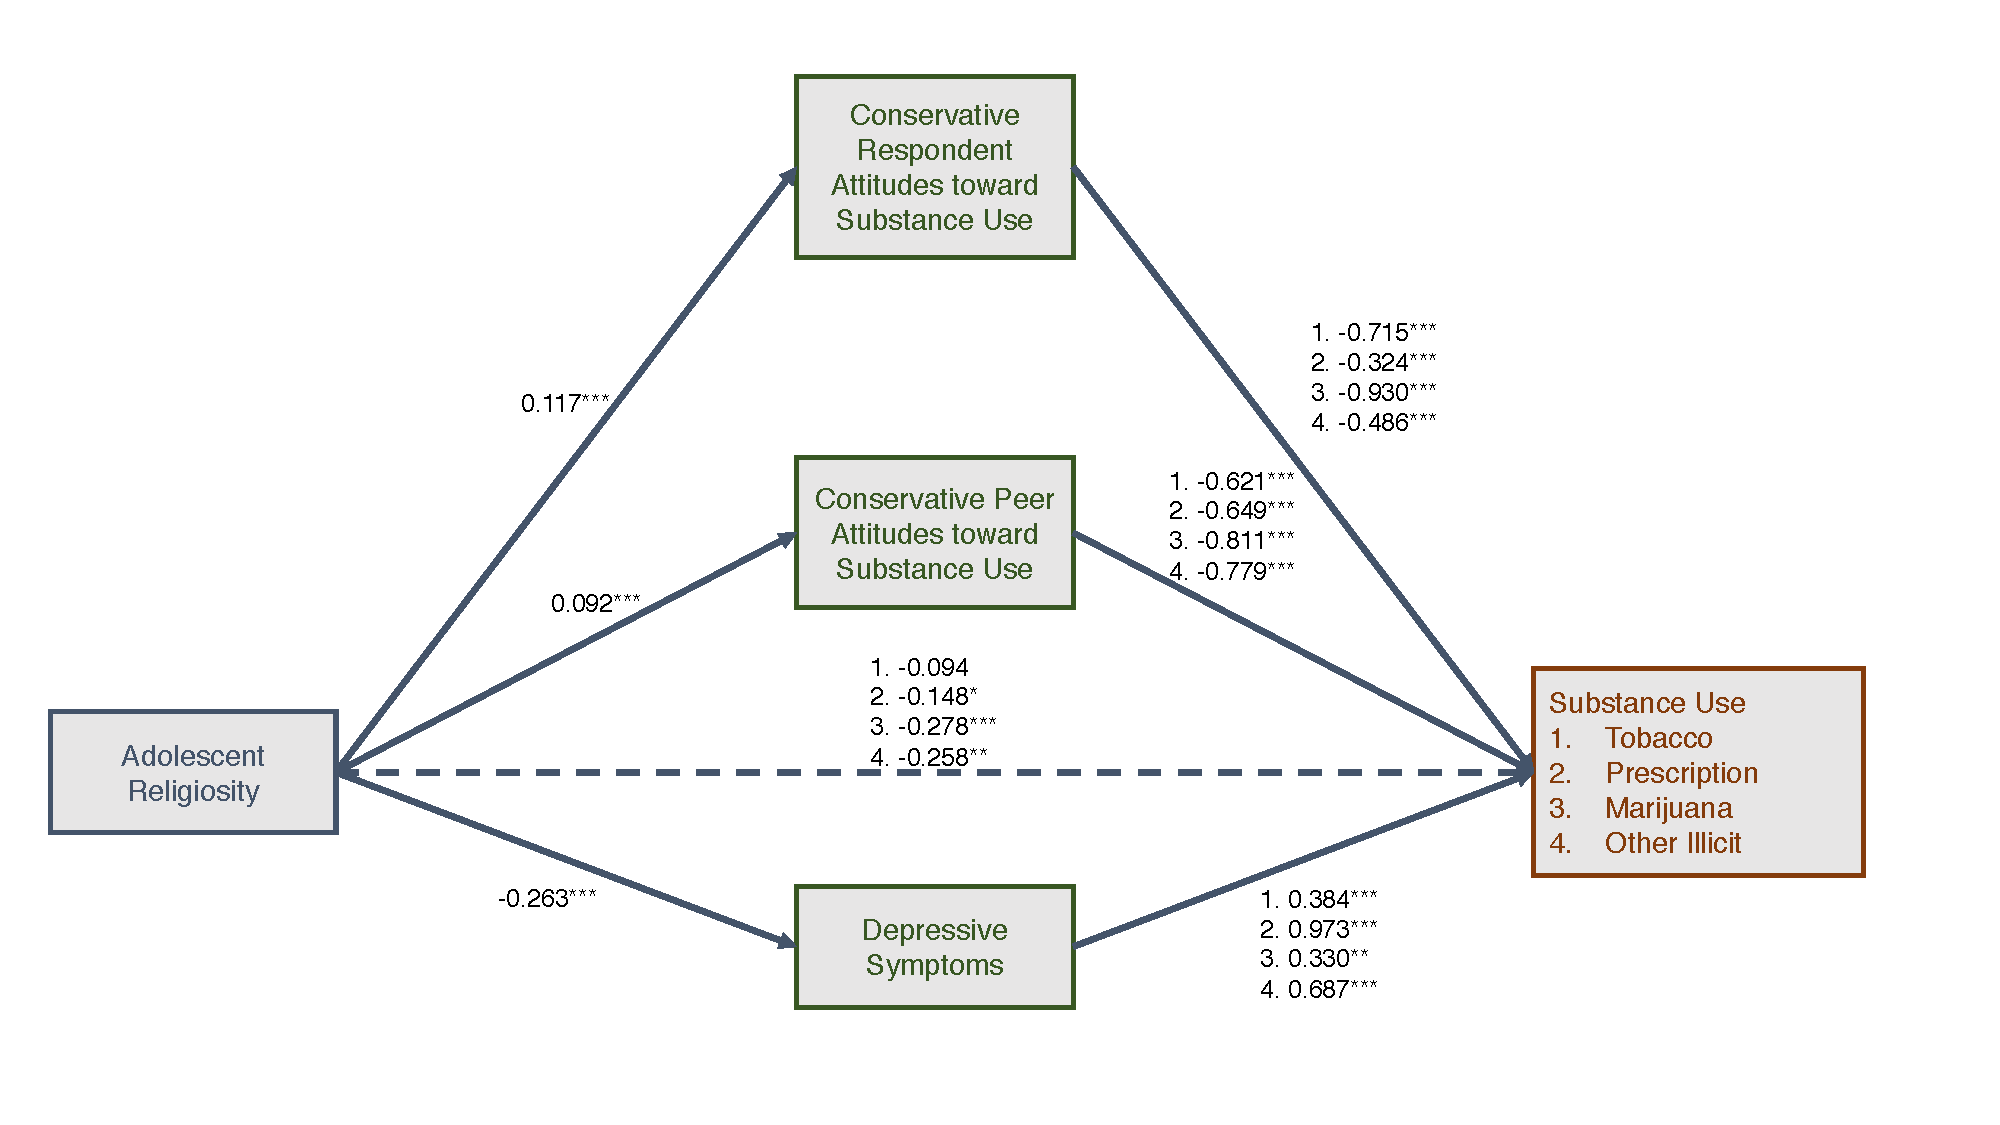
\includegraphics[width = \linewidth]{figures/fig_application_results.pdf}
\caption{Results of the mediation models' individual paths regarding religiosity and substance use. Note: *** p < .001, ** p < .01, * p < .05}
\label{fig:appresults}
\end{figure}

Because MMA provides information about each of the indirect effects
naturally in the same units, it is possible to assess the amount
mediated by each mediator while also controlling for the other mediators
in a straightforward manner---without having to fit several other models
and assess each \(c - c'\). Table \ref{tab:perc} presents the amount of
the total effect of religiosity on substance use that is mediated
through respondent conservative attitudes, peer conservative attitudes,
and depression. Overall, the effect of religiosity on substance use is
heavily mediated by the hypothesized mediators, more so for tobacco use
than the
others.\footnote{Using the approach used in Ford and Hill, the total mediated effects are slightly different than those estimated via the indirect and direct effects. This may be due to the weighting of the sample; an important area for further research into MMAs performance.}

\begin{table}[htb]
\centering
\caption{The percent of mediation (the percent of the total effect) by path for each outcome.}
\begin{tabular}{lcccc}
\toprule
            & \multicolumn{4}{c}{Outcome} \\
   Mediator & Tobacco & Prescription & Marijuana & Illicit \\ 
\midrule
Respondent Views  & 34.2  & 14.0  & 23.2 & 14.1 \\ 
Peer Views        & 23.2  & 22.0  & 15.8 & 17.7 \\ 
Depression        & 4.0   & 9.2   & 1.8  & 4.4 \\ 
Total Mediation   & 61.4  & 45.2  & 40.8 & 36.1 \\ 
\bottomrule
\end{tabular}\label{tab:perc}
\end{table}

In addition to this information, MMA provides information regarding the
indirect and direct effects in the same units. Figure \ref{fig:app}
highlights the indirect and direct effects with their associated 95\%
confidence intervals in the average marginal effects. All of the effects
here are in risk (probability) units---i.e., risk of tobacco use,
prescription misuse, marijuana use, or illicit drug use. Although all
indirect effects and most direct effects are significant, the effect
size estimates are particularly important here as the meaningfulness of
these significant effects can be overlooked.

These resulting effects are all small, with most effects less than 0.01
(i.e., less than a single risk unit). That is, most effects show changes
in the risk of the outcome by less than a single unit. For example, if
adolescent religiosity is increased by one unit, its effect on the risk
of tobacco use, through respondent attitudes, is a decrease of 0.007;
through peer attitudes a decrease of 0.005; through depression a
decrease of 0.001; and directly a decrease of 0.008. The total effect,
then, is approximately -0.021. Therefore, if an individual has a risk of
using tobacco at 50\%, by increasing religiosity by one unit (holding
the covariates constant), on average that individual's risk would
decrease to 47.9\%. About 0.013 of the effect of religiosity on tobacco
use is mediated while 0.008 is direct from religiosity. Ultimately,
these findings highlight the fact that the effect sizes, especially the
indirect and direct effect sizes, are valuable companions to the
p-values.

\begin{verbatim}
## Error in loadNamespace(name): there is no package called 'anteo'
\end{verbatim}

\section{Conclusions}\label{conclusions-3}

The replication highlighted several important facets of the important
work by Ford and Hill (2012). First, it simplifies the interpretation of
the model by using average marginal effects. Second, it highlighted the
effect sizes in terms of risk of substance use. This allowed the
relatively small effects to be understood, not only in their
significance, but in their meaning. Ultimately, MMA provided a more
straightforward approach and substantially more information for each
model than other mediation approaches.

\singlespacing

\FloatBarrier

\newpage

\fancyhead[L]{Discussion} \fancyhead[R]{\thepage} \fancyfoot[C]{}

\chapter{DISCUSSION}

\begin{quote}
\emph{A model is a simplification or approximation of reality and hence will not reflect all of reality. ... While a model can never be ``truth," a model might be ranked from very useful, to useful, to somewhat useful, to, finally, essentially useless.}
--- Burnham and Anderson, 2002
\end{quote}

\doublespacing

\section{General Discussion}\label{general-discussion}

Models are simply representations of reality. This is also true of
mediation models even though they are used to model more complex
relations. The value in using such models is generally seen in their
ability to provide opportunities for intervention or
prevention.\footnote{Although not a major aspect of this project, it is important to note the predictive power a specific model has. For example, a model may show a significant effect in a logistic regression but it may not predict the outcome above chance. In this case, the question turns from ``does X have an effect on Y?" to ``does it predict Y?" This distinction has important implications when it comes to intervention and prevention but involves a number of important concepts that cannot be covered herein (e.g., model specification including penalty parameters, modeling approach such as tree based approaches). This general idea---that of the importance of predictive accuracy---is discussed in Hastie, Tibshirani, and Friedman (2009).}

As has been discussed throughout this project, mediation models are most
useful when the model communicates both the significance (e.g.,
p-values) and meaningfulness (e.g., effect sizes). One without the other
can be misleading, potentially resulting in faulty interventions and
policies. Together, significance and meaning tell a more complete story
of the data The significance helps researchers understand uncertainty;
effect sizes communicate the potential for intervention to actually make
meaningful changes in important outcomes.

However, some situations wherein mediation analysis is applied can
provide a lack of interpretable information, particularly in terms of
the effect sizes. This limits the usefulness of the model, whether or
not it is an accurate representation of reality. It is for this purpose
that Marginal Mediation Analysis (MMA) was developed. It provides
mediation analysis with the tools to communicate both significance and
meaning. This is coming forth at an opportune time, as the American
Psychological Association, among others, have called for more focus on
effect sizes and less attention on p-values (Cumming, 2014).

\subsection{Findings from the Three
Phases}\label{findings-from-the-three-phases}

This project has presented the development of the approach and its
software, the evaluation of its performance in possible real-world
scenarios, and the application of it to health data regarding adolescent
substance use. In its first phase, this project produced MMA with its
accompanying software---the \texttt{MarginalMediation} R package. The
software is freely available and allows for researchers to quickly apply
it. The main function, \texttt{mma()}, is relatively quick even with the
bootstrapping, and produces thorough output.

The next phase used Monte Carlo simulations to evaluate MMA and ways
that it can possibly be improved. For example, given the results
regarding the confidence interval coverage, it may be of benefit to try
alternative approaches, either adaptations of bootstrapping (e.g.,
Bias-Corrected Bootstrap) or others. MacKinnon et al. (2004) found that
Monte Carlo confidence intervals performed well and, therefore, may also
be a valuable addition to MMA.

These simulations further demonstrated a trade-off regarding sample
sizes and effect sizes: large effect sizes can be found in small samples
but those same conditions provide much more variability in estimating
the total effect accurately. Overall, these findings demonstrate the
ability for the sample size, as it increases, to reduce bias and
solidify relationships that should hold in mediation models (e.g.,
\(a \times b + c' = c\)).

The Monte Carlo simulations also allowed for the testing of the
software. Some situations, once simulated, demonstrated a need for
change, often regarding the speed of the software, its accuracy, and
necessary checks to avoid more serious problems. Ultimately, there was a
natural feedback loop between the simulations and the software that were
developed interactively. Once a stable version of the software was
achieved, the reported simulations were all run based on that version
(v0.5.0).

In the final phase, the application study highlighted important
information regarding the MMA approach and adolescent health. The
application study replicated work by Ford and Hill (2012), which was
chosen to replicate for three major reasons:

\begin{enumerate}
\def\labelenumi{\arabic{enumi}.}
\tightlist
\item
  the application study used a large sample with a mix of binary and
  continuous mediators and outcomes (common in the literature),
\item
  the statistical approach is one of the better approaches (also common
  in the literature), and
\item
  the data were open and a more recent release was available to
  investigate.
\end{enumerate}

Although MMA can benefit the researcher in many situations, the benefits
of using MMA are particularly clear within the context of this
application study. Most importantly, MMA provided more information, in
the form of effect size estimates, that help instruct on the
meaningfulness of the results (Cumming, 2014). As Preacher and Kelley
(2011) state: ``it is important to develop a way to gauge the effect
size of the product term \(ab\) itself,'' (pg. 95). That is, not only
does the effect size of the individual paths need to be meaningful but
the product of \(a \times b\) must be as well. Although nearly all
effects were significant, with such a large sample size significance
tests alone can be misleading. For this study, the addition of the
effect sizes are helpful to understand that each estimated effect was
small. This provides a more complete view of the relationships tested
herein.

Second, in terms of the substantive findings, there is strong evidence
across many studies that adolescent religiosity is related to substance
use. This is shown here as well. Consistently, religiosity was
negatively related to the four substance use outcomes. About half of the
total effect of religiosity on substance use was mediated by personal
and peer attitudes about substance use. Depression also mediated the
relationship, but to a much lesser degree.

Although not definitive, this study in conjunction with Ford and Hill
(2012) presents evidence that religiosity may impact substance use
outcomes through attitudes towards substance use. More research,
particularly research with longitudinal data, are needed to further test
and understand these relationships and their ability to inform
intervention or policy.

\section{Limitations}\label{limitations}

The MMA approach has two notable limitations. First, mediation analysis
assumes no measurement error in the mediators. Although latent variable
methods can help with this (Iacobucci, 2008; Lockhart et al., 2011), the
data necessary are not always available and the integration of average
marginal effects within SEM is not clearly defined as of yet.
Ultimately, the estimates are only as good as the measurements. Second,
it may also be difficult for researchers to accept given the novelty of
average marginal effects in the field. This is being alleviated through
the use of various introductions to average marginal effects and its use
in other fields (Barrett \& Lockhart, in preparation).

Of course, the Monte Carlo simulation did not test for all conditions
present in real-world modeling. Although it accounted for the main
influences, there are other possible important influences that may
impact the performance of the method, including missing values and model
mis-specification. These are important influences to assess in future
projects. Finally, the application study used cross-sectional data. This
makes it difficult to demonstrate causality and puts additional pressure
on the ability to control for confounding.

\section{Future Research}\label{future-research}

Several foreseeable areas of investigation can prove useful for
understanding and extending MMA. First, the application highlighted an
important area for future inquiry---MMA with survey weighted data. The
application study used data that were collected via a complex survey
design and were therefore weighted. Further research is needed to
understand MMAs behavior in these situations.

Second, this project specifically assessed binary and count mediators.
Another important type of variable that could play an important role in
mediation is ``time-to-event'' or survival data. Future research is
needed to understand how this type of data with its accompanying
statistical approaches can fit into MMA.

Third, MMA relies on the \emph{sequential ignorability} assumption as
described by Imai et al. (2010a). A sensitivity analysis is available to
assess how important deviations from this assumption are on the
estimates and conclusions (Imai et al., 2010a, 2010b). Integrating this
sensitivity analysis would be a valuable addition to the approach. It
likely would be a natural integration but this integration would need to
be tested.

Relatedly, it could also be useful to look at using instrumental
variables to help appease sequential ignorability. Although generally
not applied in conjunction with mediation analysis, the approach could
prove useful for MMA specifically and mediation analysis as a whole.

Lastly, the integration of latent variable approaches, including latent
class analysis, is an important step in making this approach more
broadly applicable. Work regarding average marginal effects, categorical
data, and structural equation models would be an important contribution
as well.

\section{Conclusions}\label{conclusions-4}

The results of the development, simulations, and application all show
that MMA holds much promise in extending mediation analysis more fully
to situations where the mediators and/or outcomes are categorical or
non-normally distributed. Although further work is necessary to
understand MMAs performance across more situations, the results of this
project demonstrates its utility for common health and prevention
research.

\singlespacing

\FloatBarrier

\newpage

\fancyhead[L]{References} \fancyhead[R]{\thepage} \fancyfoot[C]{}

\chapter*{REFERENCES}

\setlength{\parindent}{-0.5in} \setlength{\leftskip}{0.4in}
\setlength{\parskip}{6pt} \noindent

\hypertarget{refs}{}
\hypertarget{ref-Bartus2005}{}
Bartus, T. (2005). Estimation of marginal effects using margeff.
\emph{Stata Journal}, \emph{5}(3), 309--329.
\href{https://doi.org/The\%20Stata\%20Journal}{https://doi.org/The Stata Journal}

\hypertarget{ref-Burnham2002}{}
Burnham, K., and Anderson, D. (2002). \emph{Model selection and
multimodel inference: A practical information-theoretic approach}.
Springer-Verlag.

\hypertarget{ref-Carsey2013}{}
Carsey, T. M., and Harden, J. J. (2013). \emph{Monte carlo simulation
and resampling methods for social science}. SAGE.

\hypertarget{ref-Catanzaro2004}{}
Catanzaro, S. J., and Laurent, J. (2004). Perceived family support,
negative mood regulation expectancies, coping, and adolescent alcohol
use: Evidence of mediation and moderation effects. \emph{Addictive
Behaviors}, \emph{29}(9), 1779--1797.
\url{https://doi.org/10.1016/j.addbeh.2004.04.001}

\hypertarget{ref-Coie1993}{}
Coie, J. D., Watt, N. F., West, S. G., Hawkins, J. D., Asarnow, J. R.,
Markman, H. J., \ldots{} Long, B. (1993). The Science of Prevention.
\emph{American Psychologist}, \emph{48}(10), 1013--1022.
\url{https://doi.org/10.1037/0003-066X.48.10.1013}

\hypertarget{ref-Cumming2014}{}
Cumming. (2014). The new statistics: Why and how. \emph{Psychological
Science}, \emph{25}(1), 7--29.
\url{https://doi.org/10.1177/0956797613504966}

\hypertarget{ref-Edwards2007}{}
Edwards, J. R., and Lambert, L. S. (2007). Methods for integrating
moderation and mediation: a general analytical framework using moderated
path analysis. \emph{Psychological Methods}, \emph{12}(1), 1--22.
\url{https://doi.org/10.1037/1082-989X.12.1.1}

\hypertarget{ref-Ennett2001}{}
Ennett, S. T., Bauman, K. E., Pemberton, M., Foshee, V. a, Chuang, Y.
C., King, T. S., and Koch, G. G. (2001). Mediation in a family-directed
program for prevention of adolescent tobacco and alcohol use.
\emph{Preventive Medicine}, \emph{33}(4), 333--46.
\url{https://doi.org/10.1006/pmed.2001.0892}

\hypertarget{ref-Fairchild2009}{}
Fairchild, A. J., and MacKinnon, D. P. (2009). A general model for
testing mediation and moderation effects. \emph{Prevention Science},
\emph{10}(2), 87--99. \url{https://doi.org/10.1007/s11121-008-0109-6}

\hypertarget{ref-Ford2012}{}
Ford, J. A., and Hill, T. D. (2012). Religiosity and Adolescent
Substance Use: Evidence From the National Survey on Drug Use and Health.
\emph{Substance Use \& Misuse}, \emph{47}(7), 787--798.
\url{https://doi.org/10.3109/10826084.2012.667489}

\hypertarget{ref-Graham2007}{}
Graham, J. W., Olchowski, A. E., and Gilreath, T. D. (2007). How many
imputations are really needed? Some practical clarifications of multiple
imputation theory. \emph{Prevention Science}, \emph{8}(3), 206--213.
\url{https://doi.org/10.1007/s11121-007-0070-9}

\hypertarget{ref-Hastie2009}{}
Hastie, T., Tibshirani, R., and Friedman, J. (2009). \emph{The Elements
of Statistical Learning} (Vol. 1). \url{https://doi.org/10.1007/b94608}

\hypertarget{ref-Hayes2009}{}
Hayes, A. F. (2009). Beyond Baron and Kenny: Statistical Mediation
Analysis in the New Millennium. \emph{Statistical Mediation Analysis in
the New Millennium}, \emph{76}(4), 408--420.
\url{https://doi.org/10.1080/03637750903310360}

\hypertarget{ref-Hayes2013book}{}
Hayes, A. F. (2013). \emph{Introduction to mediation, moderation, and
conditional process analysis: A regression-based approach}. The Guilford
Press.

\hypertarget{ref-intelbook1999}{}
Heuer Jr., R. J. (1999). \emph{Psychology of intelligence analysis}.
Center for the Study of Intelligence.

\hypertarget{ref-Hoeppner2017}{}
Hoeppner, B., Hoeppner, S., and Abroms, L. (2017). How do text-messaging
smoking cessation interventions confer benefit? A multiple mediation
analysis of Text2Quit. \emph{Addiction}, 673--682.
\url{https://doi.org/10.1111/add.13685}

\hypertarget{ref-Hofler2005}{}
Hofler, M. (2005). Causal inference based on counterfactuals. \emph{BMC
Medical Research Methodology}, \emph{5}(28), 1--12.
\url{https://doi.org/10.1186/1471-2288-5-28}

\hypertarget{ref-Iacobucci2008book}{}
Iacobucci, D. (2008). \emph{Mediation analysis}. SAGE {[}Kindle
Version{]}.

\hypertarget{ref-Iacobucci2012}{}
Iacobucci, D. (2012). Mediation analysis and categorical variables: The
final frontier. \emph{Journal of Consumer Psychology}, \emph{22}(4),
582--594. \url{https://doi.org/10.1016/j.jcps.2012.03.006}

\hypertarget{ref-Iacobucci2007}{}
Iacobucci, D., Saldanha, N., and Deng, X. (2007). A mediation on
mediation: Evidence that structural equation models perform better than
regression. \emph{Journal of Consumer Psychological}, \emph{7}(2),
140--154. \url{https://doi.org/10.1016/S1057-7408(07)70020-7}

\hypertarget{ref-Imai2010a}{}
Imai, K., Keele, L., and Tingley, D. (2010a). A general approach to
causal mediation analysis. \emph{Psychological Methods}, \emph{15}(4),
309--34. \url{https://doi.org/10.1037/a0020761}

\hypertarget{ref-Imai2010b}{}
Imai, K., Keele, L., and Yamamoto, T. (2010b). Identification, Inference
and Sensitivity Analysis for Causal Mediation Effects. \emph{Statistical
Science}, \emph{25}(1), 51--71. \url{https://doi.org/10.1214/10-STS321}

\hypertarget{ref-Jiang2015}{}
Jiang, Z., and Vanderweele, T. (2015). When is the difference method
conservative for assessing mediation? \emph{American Journal of
Epidemiology}, \emph{182}(2), 105--108.
\url{https://doi.org/10.1093/aje/kwv059}

\hypertarget{ref-Leeper2017}{}
Leeper, T. J. (2017). \emph{Interpreting Regression Results using
Average Marginal Effects with R's margins} (pp. 1--31). Retrieved from
\url{https://cran.r-project.org/web/packages/margins/vignettes/TechnicalDetails.pdf}

\hypertarget{ref-Lockhart2011}{}
Lockhart, G., Mackinnon, D. P., and Ohlrich, V. (2011). Mediation
analysis in psychosomatic medicine research. \emph{Psychosomatic
Medicine}, \emph{73}(1), 29--43.
\url{https://doi.org/10.1097/PSY.0b013e318200a54b.Mediation}

\hypertarget{ref-Lockhart2017}{}
Lockhart, G., Phillips, S., Bolland, A., Delgado, M., Tietjen, J., and
Bolland, J. (2017). Prospective Relations among Low-Income African
American Adolescents' Maternal Attachment Security, Self-Worth, and Risk
Behaviors. \emph{Frontiers in Psychology}, \emph{8}(January), 1--10.
\url{https://doi.org/10.3389/fpsyg.2017.00033}

\hypertarget{ref-Loken2017}{}
Loken, E., and Gelman, A. (2017). Measurement error and the replication
crisis. \emph{Science}, \emph{355}(6325), 584--585.
\url{https://doi.org/10.1126/science.aal3618}

\hypertarget{ref-Luk2010}{}
Luk, J. W., Wang, J., and Simons-Morton, B. G. (2010). Bullying
Victimization and Substance Use Among U.S. Adolescents: Mediation by
Depression. \emph{Prevention Science}, \emph{11}(4), 355--359.
\url{https://doi.org/10.1007/s11121-010-0179-0}

\hypertarget{ref-mackinnon2008intro}{}
MacKinnon, D. P. (2008). \emph{Introduction to statistical mediation
analysis}. Routledge.

\hypertarget{ref-MacKinnon2012}{}
MacKinnon, D. P., and Cox, M. C. (2012). Commentary on ``Mediation
Analysis and Categorical Variables: The Final Frontier'' by Dawn
Iacobucci. \emph{Journal of Consumer Psychology}, \emph{22}(4),
600--602. \url{https://doi.org/10.1016/j.jcps.2012.03.009.Commentary}

\hypertarget{ref-MacKinnon2007}{}
MacKinnon, D. P., Fairchild, A. J., and Fritz, M. (2007). Mediation
Analysis. \emph{Annual Review of Psychology}, \emph{58}(Hebb 1966),
593--602.
\url{https://doi.org/10.1146/annurev.psych.58.110405.085542.Mediation}

\hypertarget{ref-MacKinnon2004}{}
MacKinnon, D. P., Lockwood, C. M., and Williams, J. (2004). Confidence
Limits for the Indirect Effect: Distribution of the Product and
Resampling Methods. \emph{Multivariate Behavioral Research},
\emph{39}(1). \url{https://doi.org/10.1207/s15327906mbr3901_4}

\hypertarget{ref-Montreuil2005}{}
Montreuil, B., Bendavid, Y., and Brophy, J. (2005). What is so odd about
odds? \emph{J Can Chir}, \emph{48}(5), 400--408.

\hypertarget{ref-Mood2010}{}
Mood, C. (2010). Logistic regression: Why we cannot do what We think we
can do, and what we can do about it. \emph{European Sociological
Review}, \emph{26}(1), 67--82. \url{https://doi.org/10.1093/esr/jcp006}

\hypertarget{ref-Muthen1984}{}
Muthén, B. (1984). A general structural equation model with dichotomous,
ordered categorical, and continuous latent variable indictors.
\emph{Psychometrika}, \emph{49}(1), 115--132.

\hypertarget{ref-Norton2012}{}
Norton, E. C. (2012). \emph{Log Odds and Ends}. National Bureau of
Economic Research. \url{https://doi.org/10.1002/0471725331.ch16}

\hypertarget{ref-Nylund2007}{}
Nylund, K. L., Asparouhov, T., and Muthen, B. O. (2007). Deciding on the
number of classes in latent class analysis and growth mixture modeling:
A Monte Carlo simulation study. \emph{Structural Equation Modeling},
\emph{15}(1), 182. \url{https://doi.org/10.1080/10705510701575396}

\hypertarget{ref-Paxton2001}{}
Paxton, P., Curran, P. J., Bollen, K. a., Kirby, J., and Chen, F.
(2001). Monte Carlo Experiments: Design and Implementation.
\emph{Structural Equation Modeling: A Multidisciplinary Journal},
\emph{8}(2), 287--312. \url{https://doi.org/10.1207/S15328007SEM0802_7}

\hypertarget{ref-Pinquart2011}{}
Pinquart, M., and Shen, Y. (2011). Behavior problems in children and
adolescents with chronic physical illness: A meta-analysis.
\emph{Journal of Pediatric Psychology}, \emph{36}(4), 375--384.
\url{https://doi.org/http://dx.doi.org/10.1093/jpepsy/jsq104}

\hypertarget{ref-Preacher2011}{}
Preacher, K. J., and Kelley, K. (2011). Effect Size Measures for
Mediation Models : Quantitative Strategies for Communicating Indirect
Effects, \emph{16}(2), 93--115. \url{https://doi.org/10.1037/a0022658}

\hypertarget{ref-Serang2017}{}
Serang, S., Jacobucci, R., Brimhall, K. C., and Grimm, K. J. (2017).
Exploratory Mediation Analysis via Regularization. \emph{Structural
Equation Modeling: A Multidisciplinary Journal}, 1--12.
\url{https://doi.org/10.1080/10705511.2017.1311775}

\hypertarget{ref-Shih2010}{}
Shih, R. A., Miles, J. N. V., Tucker, J. S., Zhou, A. J., D 'amico, E.
J., Jeremy, R. O., and Miles, N. V. (2010). Racial/Ethnic Differences in
Adolescent Substance Use: Mediation by Individual, Family, and School
Factors*. \emph{JOURNAL OF STUDIES ON ALCOHOL AND DRUGS / SEPTEMBER 2010
Stud. Alcohol Drugs}, \emph{71}(September), 640--651.
\url{https://doi.org/10.15288/jsad.2010.71.640}

\hypertarget{ref-Shrout2002}{}
Shrout, P. E., and Bolger, N. (2002). Mediation in experimental and
nonexperimental studies: new procedures and recommendations.
\emph{Psychological Methods}, \emph{7}(4), 422.
\url{https://doi.org/10.1037//1082-989x.7.4.422}

\hypertarget{ref-Small2013}{}
Small, D. S. (2013). \emph{Mediation Analysis Without Sequential
Ignorability: Using Baseline Covariates Interacted with Random
Assignment as Instrumental Variables}.

\hypertarget{ref-Sobel1982}{}
Sobel, M. E. (1982). Asymptotic Confidence Intervals for Indirect
Effects in Structural Equation Models. \emph{Sociological Methodology},
\emph{13}, 290--312.

\hypertarget{ref-Stata14}{}
StataCorp. (2015). \emph{Stata Statistical Software: Release 14}.
StataCorp LLC.

\hypertarget{ref-Wang2009}{}
Wang, J., Simons-Morton, B. G., Farhart, T., and Luk, J. W. (2009).
Socio-demographic variability in adolescent substance use: Mediation by
parents and peers. \emph{Prevention Science}, \emph{10}(4), 387--396.
\url{https://doi.org/10.1007/s11121-009-0141-1}

\hypertarget{ref-Wickham2015}{}
Wickham, H. (2015). \emph{R Packages: Organize, Test, Document, and
Share Your Code} (1st ed.). O'Reilly Media.

\hypertarget{ref-Winship1983}{}
Winship, C., and Mare, R. (1983). Structural Equations and Path Analysis
for Discrete Data. \emph{The American Journal of Sociology},
\emph{89}(1), 54--110.

\hypertarget{ref-Wong2013}{}
Wong, M. M., and Brower, K. J. (2013). The prospective relationship
between sleep problems and suicidal behavior in the National
Longitudinal Study of Adolescent Health. \emph{Journal of Psychiatric
Research}, \emph{46}(7), 953--959.
\url{https://doi.org/10.1016/j.jpsychires.2012.04.008.The}

\clearpage
\addcontentsline{toc}{chapter}{APPENDICES} \fancyhead[L]{Appendices}
\fancyhead[R]{\thepage} \fancyfoot[C]{}

\vspace*{\fill}

\begin{center}
    APPENDICES 
  \end{center}

\vspace*{\fill}

\clearpage

\doublespacing

\section*{Appendix A: R Code for Chapter
5}\label{appendix-a-r-code-for-chapter-5}
\addcontentsline{toc}{section}{Appendix A: R Code for Chapter 5}

\singlespace

Required: R Packages from CRAN

\small

\begin{Shaded}
\begin{Highlighting}[]
\ControlFlowTok{if}\NormalTok{ (}\OperatorTok{!}\KeywordTok{require}\NormalTok{(tidyverse))\{}
  \KeywordTok{install.packages}\NormalTok{(}\StringTok{"tidyverse"}\NormalTok{)}
  \KeywordTok{library}\NormalTok{(tidyverse)}
\NormalTok{\}}
\ControlFlowTok{if}\NormalTok{ (}\OperatorTok{!}\KeywordTok{require}\NormalTok{(furniture))\{}
  \KeywordTok{install.packages}\NormalTok{(}\StringTok{"furniture"}\NormalTok{)}
  \KeywordTok{library}\NormalTok{(furniture)}
\NormalTok{\}}
\ControlFlowTok{if}\NormalTok{ (}\OperatorTok{!}\KeywordTok{require}\NormalTok{(here))\{}
  \KeywordTok{install.packages}\NormalTok{(}\StringTok{"here"}\NormalTok{)}
  \KeywordTok{library}\NormalTok{(here)}
\NormalTok{\}}
\ControlFlowTok{if}\NormalTok{ (}\OperatorTok{!}\KeywordTok{require}\NormalTok{(devtools))\{}
  \KeywordTok{install.packages}\NormalTok{(}\StringTok{"devtools"}\NormalTok{)}
  \KeywordTok{library}\NormalTok{(devtools)}
\NormalTok{\}}
\end{Highlighting}
\end{Shaded}

\normalsize

Required: R Packages from GitHub

\small

\begin{Shaded}
\begin{Highlighting}[]
\ControlFlowTok{if}\NormalTok{ (}\OperatorTok{!}\KeywordTok{require}\NormalTok{(MarginalMediation))\{}
\NormalTok{  devtools}\OperatorTok{::}\KeywordTok{install_github}\NormalTok{(}\StringTok{"tysonstanley/MarginalMediation"}\NormalTok{)}
  \KeywordTok{library}\NormalTok{(MarginalMediation)}
\NormalTok{\}}
\end{Highlighting}
\end{Shaded}

\normalsize

\clearpage

\subsection*{Examples from Chapter 5}\label{examples-from-chapter-5}
\addcontentsline{toc}{subsection}{Examples from Chapter 5}

Figure \ref{fig:interaction} on page \pageref{fig:interaction}

\small

\begin{Shaded}
\begin{Highlighting}[]
\KeywordTok{set.seed}\NormalTok{(}\DecValTok{843}\NormalTok{)}
\KeywordTok{library}\NormalTok{(tidyverse)}
\NormalTok{tibble}\OperatorTok{::}\KeywordTok{data_frame}\NormalTok{(}
  \DataTypeTok{X =} \KeywordTok{rnorm}\NormalTok{(}\DecValTok{100}\NormalTok{),}
  \DataTypeTok{W =} \KeywordTok{rbinom}\NormalTok{(}\DecValTok{100}\NormalTok{, }\DecValTok{1}\NormalTok{, .}\DecValTok{5}\NormalTok{),}
  \DataTypeTok{Y =}\NormalTok{ X }\OperatorTok{+}\StringTok{ }\NormalTok{.}\DecValTok{5}\OperatorTok{*}\NormalTok{W }\OperatorTok{+}\StringTok{ }\OperatorTok{-}\NormalTok{.}\DecValTok{5}\OperatorTok{*}\NormalTok{X}\OperatorTok{*}\NormalTok{W }\OperatorTok{+}\StringTok{ }\KeywordTok{rnorm}\NormalTok{(}\DecValTok{100}\NormalTok{)}
\NormalTok{) }\OperatorTok
\StringTok{  }\KeywordTok{ggplot}\NormalTok{(}\KeywordTok{aes}\NormalTok{(X, Y, }\DataTypeTok{group =} \KeywordTok{factor}\NormalTok{(W), }\DataTypeTok{color =} \KeywordTok{factor}\NormalTok{(W))) }\OperatorTok{+}
\StringTok{    }\KeywordTok{geom_point}\NormalTok{(}\DataTypeTok{alpha =}\NormalTok{ .}\DecValTok{3}\NormalTok{) }\OperatorTok{+}
\StringTok{    }\KeywordTok{geom_smooth}\NormalTok{(}\DataTypeTok{method =} \StringTok{"lm"}\NormalTok{, }\DataTypeTok{se=}\OtherTok{FALSE}\NormalTok{) }\OperatorTok{+}
\StringTok{    }\KeywordTok{scale_color_manual}\NormalTok{(}\DataTypeTok{values =} \KeywordTok{c}\NormalTok{(}\StringTok{"dodgerblue4"}\NormalTok{, }\StringTok{"chartreuse4"}\NormalTok{)) }\OperatorTok{+}
\StringTok{    }\KeywordTok{labs}\NormalTok{(}\DataTypeTok{color =} \StringTok{"Moderator"}\NormalTok{) }\OperatorTok{+}
\StringTok{    }\NormalTok{anteo}\OperatorTok{::}\KeywordTok{theme_anteo_wh}\NormalTok{()}
\KeywordTok{ggsave}\NormalTok{(}\StringTok{"figures/fig_interaction_effect.pdf"}\NormalTok{, }
       \DataTypeTok{width =} \DecValTok{7}\NormalTok{, }\DataTypeTok{height =} \DecValTok{5}\NormalTok{, }\DataTypeTok{units =} \StringTok{"in"}\NormalTok{)}
\end{Highlighting}
\end{Shaded}

\normalsize

\clearpage

\subsection*{Monte Carlo Simulation}\label{monte-carlo-simulation}
\addcontentsline{toc}{subsection}{Monte Carlo Simulation}

Notably, the code for both the binary mediator condition and the count
mediator condition we run via the Terminal as, once the directory was
where the R file was located:

\small

\begin{Shaded}
\begin{Highlighting}[]
\ExtensionTok{Rscript}\NormalTok{ Analyses_MMMC_scriptBinary.R }\StringTok{'c(1:45)'}
\end{Highlighting}
\end{Shaded}

\normalsize

\noindent and

\small

\begin{Shaded}
\begin{Highlighting}[]
\ExtensionTok{Rscript}\NormalTok{ Analyses_MMMC_scriptCount.R }\StringTok{'c(1:45)'}
\end{Highlighting}
\end{Shaded}

\normalsize

Binary Mediator

\small

\begin{Shaded}
\begin{Highlighting}[]
\NormalTok{## Marginal Mediation: Monte Carlo Simulation Study}
\NormalTok{##   BINARY Mediator}
\NormalTok{## Tyson S. Barrett}
\NormalTok{##}
\NormalTok{## devtools::install_github("tysonstanley/MarginalMediation")}

\NormalTok{args <-}\StringTok{ }\KeywordTok{commandArgs}\NormalTok{(}\OtherTok{TRUE}\NormalTok{)}
\NormalTok{args <-}\StringTok{ }\KeywordTok{eval}\NormalTok{(}\KeywordTok{parse}\NormalTok{(}\DataTypeTok{text =}\NormalTok{ args))}
\KeywordTok{library}\NormalTok{(MarginalMediation)}
\KeywordTok{library}\NormalTok{(tidyverse)}

\NormalTok{## Create all combinations of independent variables}
\NormalTok{cond_binary =}\StringTok{ }\KeywordTok{expand.grid}\NormalTok{(}
  \DataTypeTok{samplesize =} \KeywordTok{c}\NormalTok{(}\DecValTok{50}\NormalTok{, }\DecValTok{100}\NormalTok{, }\DecValTok{200}\NormalTok{, }\DecValTok{500}\NormalTok{, }\DecValTok{1000}\NormalTok{),}
  \DataTypeTok{effecta    =} \KeywordTok{c}\NormalTok{(.}\DecValTok{55}\NormalTok{, }\FloatTok{1.45}\NormalTok{, }\FloatTok{2.22}\NormalTok{),}
  \DataTypeTok{effectb    =} \KeywordTok{c}\NormalTok{(.}\DecValTok{24}\NormalTok{, .}\DecValTok{62}\NormalTok{, }\FloatTok{1.068}\NormalTok{),}
  \DataTypeTok{effectc    =} \KeywordTok{c}\NormalTok{(.}\DecValTok{3}\NormalTok{)}
\NormalTok{)}

\NormalTok{## Population Models}
\NormalTok{## Binary Mediator}
\NormalTok{data_genB =}\StringTok{ }\ControlFlowTok{function}\NormalTok{(ps, reps, samplesize, effecta, effectb, effectc)\{}
  \KeywordTok{set.seed}\NormalTok{(}\DecValTok{84322}\NormalTok{)}
\NormalTok{  Xc =}\StringTok{ }\KeywordTok{rnorm}\NormalTok{(ps)}
\NormalTok{  z  =}\StringTok{ }\NormalTok{effecta}\OperatorTok{*}\NormalTok{Xc }\OperatorTok{+}\StringTok{ }\KeywordTok{rnorm}\NormalTok{(ps, }\DecValTok{0}\NormalTok{, }\DecValTok{1}\NormalTok{)}
\NormalTok{  pr =}\StringTok{ }\DecValTok{1}\OperatorTok{/}\NormalTok{(}\DecValTok{1}\OperatorTok{+}\KeywordTok{exp}\NormalTok{(}\OperatorTok{-}\NormalTok{z))}
\NormalTok{  M  =}\StringTok{ }\KeywordTok{rbinom}\NormalTok{(ps, }\DecValTok{1}\NormalTok{, pr)}
\NormalTok{  Y  =}\StringTok{ }\NormalTok{effectb}\OperatorTok{*}\NormalTok{M }\OperatorTok{+}\StringTok{ }\NormalTok{effectc}\OperatorTok{*}\NormalTok{Xc }\OperatorTok{+}\StringTok{ }\KeywordTok{rnorm}\NormalTok{(ps, }\DecValTok{0}\NormalTok{, }\DecValTok{1}\NormalTok{)}
\NormalTok{  M  =}\StringTok{ }\KeywordTok{factor}\NormalTok{(M)}
\NormalTok{  df =}\StringTok{ }\KeywordTok{data.frame}\NormalTok{(Y, M, Xc)}
\NormalTok{  bin =}\StringTok{ }\KeywordTok{vector}\NormalTok{(}\StringTok{"list"}\NormalTok{, reps)}
  
  \KeywordTok{print}\NormalTok{(}\KeywordTok{cbind}\NormalTok{(samplesize, effecta, effectb))}
  \KeywordTok{print}\NormalTok{(}\KeywordTok{lm}\NormalTok{(Y }\OperatorTok{~}\StringTok{ }\NormalTok{M }\OperatorTok{+}\StringTok{ }\NormalTok{Xc)}\OperatorTok{$}\NormalTok{coefficients)}
  \KeywordTok{print}\NormalTok{(}\KeywordTok{lm}\NormalTok{(}\KeywordTok{scale}\NormalTok{(Y) }\OperatorTok{~}\StringTok{ }\NormalTok{M }\OperatorTok{+}\StringTok{ }\NormalTok{Xc)}\OperatorTok{$}\NormalTok{coefficients)}
\NormalTok{  med =}\StringTok{ }\KeywordTok{amed}\NormalTok{(}\KeywordTok{glm}\NormalTok{(M }\OperatorTok{~}\StringTok{ }\NormalTok{Xc, df, }\DataTypeTok{family =} \StringTok{"binomial"}\NormalTok{))}
  
  \ControlFlowTok{for}\NormalTok{ (i }\ControlFlowTok{in} \DecValTok{1}\OperatorTok{:}\NormalTok{reps)\{}
\NormalTok{    d =}\StringTok{ }\NormalTok{df[}\KeywordTok{sample}\NormalTok{(ps, samplesize), ]}
\NormalTok{    pathbc =}\StringTok{ }\KeywordTok{glm}\NormalTok{(Y }\OperatorTok{~}\StringTok{ }\NormalTok{M }\OperatorTok{+}\StringTok{ }\NormalTok{Xc, }\DataTypeTok{data =}\NormalTok{ d)}
\NormalTok{    patha  =}\StringTok{ }\KeywordTok{glm}\NormalTok{(M }\OperatorTok{~}\StringTok{ }\NormalTok{Xc, }\DataTypeTok{data =}\NormalTok{ d, }\DataTypeTok{family =} \StringTok{"binomial"}\NormalTok{)}
\NormalTok{    bin[[i]] =}\StringTok{ }\KeywordTok{mma}\NormalTok{(pathbc, patha,}
          \DataTypeTok{ind_effects =} \KeywordTok{c}\NormalTok{(}\StringTok{"Xc-M"}\NormalTok{),}
          \DataTypeTok{boot =} \DecValTok{500}\NormalTok{)}
\NormalTok{    bin[[i]] =}\StringTok{ }\KeywordTok{list}\NormalTok{(}\StringTok{"IndEffects"}\NormalTok{ =}\StringTok{ }\NormalTok{bin[[i]]}\OperatorTok{$}\NormalTok{ind_effects, }
                    \StringTok{"DirEffects"}\NormalTok{ =}\StringTok{ }\NormalTok{bin[[i]]}\OperatorTok{$}\NormalTok{dir_effects, }
                    \StringTok{"Boot"}\NormalTok{       =}\StringTok{ }\NormalTok{bin[[i]]}\OperatorTok{$}\NormalTok{boot, }
                    \StringTok{"Total"}\NormalTok{      =}\StringTok{ }\KeywordTok{lm}\NormalTok{(Y }\OperatorTok{~}\StringTok{ }\NormalTok{Xc, d)}\OperatorTok{$}\NormalTok{coefficients,}
                    \StringTok{"MedSize"}\NormalTok{    =}\StringTok{ }\NormalTok{med)}
    \KeywordTok{cat}\NormalTok{(}\StringTok{"}\CharTok{\textbackslash{}r}\StringTok{"}\NormalTok{, i)}
\NormalTok{  \}}
  \KeywordTok{print}\NormalTok{(}\KeywordTok{exp}\NormalTok{(}\KeywordTok{glm}\NormalTok{(M }\OperatorTok{~}\StringTok{ }\NormalTok{Xc, }\DataTypeTok{family =} \StringTok{"binomial"}\NormalTok{)}\OperatorTok{$}\NormalTok{coefficients))}
  \KeywordTok{return}\NormalTok{(bin)}
\NormalTok{\}}

\NormalTok{i =}\StringTok{ }\DecValTok{0}
\ControlFlowTok{for}\NormalTok{ (j }\ControlFlowTok{in}\NormalTok{ args)\{}
  \KeywordTok{set.seed}\NormalTok{(}\DecValTok{84322}\NormalTok{)}
\NormalTok{  i =}\StringTok{ }\NormalTok{i }\OperatorTok{+}\StringTok{ }\DecValTok{1}
  \KeywordTok{cat}\NormalTok{(}\StringTok{"}\CharTok{\textbackslash{}n}\StringTok{Number:"}\NormalTok{, j, }\StringTok{"}\CharTok{\textbackslash{}n\textbackslash{}n}\StringTok{"}\NormalTok{)}
  
\NormalTok{  out =}\StringTok{ }\KeywordTok{data_genB}\NormalTok{(}\FloatTok{1e6}\NormalTok{, }\DecValTok{500}\NormalTok{, }
\NormalTok{                  cond_binary[args[[i]],}\DecValTok{1}\NormalTok{], }
\NormalTok{                  cond_binary[args[[i]],}\DecValTok{2}\NormalTok{], }
\NormalTok{                  cond_binary[args[[i]],}\DecValTok{3}\NormalTok{], }
\NormalTok{                  cond_binary[args[[i]],}\DecValTok{4}\NormalTok{])}
  
  \KeywordTok{save}\NormalTok{(out, }\DataTypeTok{file =} \KeywordTok{paste0}\NormalTok{(}\StringTok{"Sims_Data/Binary2_"}\NormalTok{, }
\NormalTok{                          cond_binary[args[[i]],}\DecValTok{1}\NormalTok{], }\StringTok{"_"}\NormalTok{,}
\NormalTok{                          cond_binary[args[[i]],}\DecValTok{2}\NormalTok{], }\StringTok{"_"}\NormalTok{,}
\NormalTok{                          cond_binary[args[[i]],}\DecValTok{3}\NormalTok{], }\StringTok{"_"}\NormalTok{,}
\NormalTok{                          cond_binary[args[[i]],}\DecValTok{4}\NormalTok{], }\StringTok{".rda"}\NormalTok{))}
  
  \KeywordTok{cat}\NormalTok{(}\StringTok{"}\CharTok{\textbackslash{}n}\StringTok{Number:"}\NormalTok{, j, }\StringTok{"}\CharTok{\textbackslash{}n\textbackslash{}n}\StringTok{"}\NormalTok{)}
  \KeywordTok{cat}\NormalTok{(}\StringTok{"}\CharTok{\textbackslash{}n}\StringTok{Conditions Complete:}\CharTok{\textbackslash{}n}\StringTok{"}\NormalTok{,}
      \StringTok{" Sample size ="}\NormalTok{, cond_binary[args[[i]],}\DecValTok{1}\NormalTok{], }
      \StringTok{"}\CharTok{\textbackslash{}n}\StringTok{  A path      ="}\NormalTok{, cond_binary[args[[i]],}\DecValTok{2}\NormalTok{], }
      \StringTok{"}\CharTok{\textbackslash{}n}\StringTok{  B path      ="}\NormalTok{, cond_binary[args[[i]],}\DecValTok{3}\NormalTok{], }
      \StringTok{"}\CharTok{\textbackslash{}n}\StringTok{  C path      ="}\NormalTok{, cond_binary[args[[i]],}\DecValTok{4}\NormalTok{], }\StringTok{"}\CharTok{\textbackslash{}n}\StringTok{"}\NormalTok{)}
\NormalTok{\}}
\end{Highlighting}
\end{Shaded}

\normalsize

Count Mediator

\small

\begin{Shaded}
\begin{Highlighting}[]
\NormalTok{## Marginal Mediation: Monte Carlo Simulation Study}
\NormalTok{##   COUNT Mediator}
\NormalTok{## Tyson S. Barrett}
\NormalTok{##}
\NormalTok{## devtools::install_github("tysonstanley/MarginalMediation")}

\NormalTok{args <-}\StringTok{ }\KeywordTok{commandArgs}\NormalTok{(}\OtherTok{TRUE}\NormalTok{)}
\NormalTok{args <-}\StringTok{ }\KeywordTok{eval}\NormalTok{(}\KeywordTok{parse}\NormalTok{(}\DataTypeTok{text =}\NormalTok{ args))}
\KeywordTok{library}\NormalTok{(MarginalMediation)}
\KeywordTok{library}\NormalTok{(tidyverse)}

\NormalTok{## Create all combinations of independent variables}
\NormalTok{cond_count =}\StringTok{ }\KeywordTok{expand.grid}\NormalTok{(}
  \DataTypeTok{samplesize =} \KeywordTok{c}\NormalTok{(}\DecValTok{50}\NormalTok{, }\DecValTok{100}\NormalTok{, }\DecValTok{200}\NormalTok{, }\DecValTok{500}\NormalTok{, }\DecValTok{1000}\NormalTok{),}
  \DataTypeTok{effecta    =} \KeywordTok{c}\NormalTok{(.}\DecValTok{3}\NormalTok{, .}\DecValTok{6}\NormalTok{, }\FloatTok{1.1}\NormalTok{),}
  \DataTypeTok{effectb    =} \KeywordTok{c}\NormalTok{(.}\DecValTok{084}\NormalTok{, .}\DecValTok{265}\NormalTok{, .}\DecValTok{49}\NormalTok{),}
  \DataTypeTok{effectc    =} \KeywordTok{c}\NormalTok{(}\DecValTok{0}\NormalTok{, .}\DecValTok{3}\NormalTok{)}
\NormalTok{)}

\NormalTok{## Population Models}
\NormalTok{## Count Mediator}
\NormalTok{data_genC =}\StringTok{ }\ControlFlowTok{function}\NormalTok{(ps, reps, samplesize, effecta, effectb, effectc)\{}
  \KeywordTok{set.seed}\NormalTok{(}\DecValTok{84322}\NormalTok{)}
\NormalTok{  Xc =}\StringTok{ }\KeywordTok{rnorm}\NormalTok{(ps)}
\NormalTok{  m1 =}\StringTok{ }\KeywordTok{exp}\NormalTok{(effecta }\OperatorTok{*}\StringTok{ }\NormalTok{Xc)}
\NormalTok{  M  =}\StringTok{ }\KeywordTok{rpois}\NormalTok{(ps, }\DataTypeTok{lambda=}\NormalTok{m1)}
\NormalTok{  Y  =}\StringTok{ }\NormalTok{effectb}\OperatorTok{*}\NormalTok{M }\OperatorTok{+}\StringTok{ }\NormalTok{effectc}\OperatorTok{*}\NormalTok{Xc }\OperatorTok{+}\StringTok{ }\KeywordTok{rnorm}\NormalTok{(ps, }\DecValTok{0}\NormalTok{, }\DecValTok{1}\NormalTok{)}
\NormalTok{  df =}\StringTok{ }\KeywordTok{data.frame}\NormalTok{(Y, M, Xc)}
\NormalTok{  poi  =}\StringTok{ }\KeywordTok{vector}\NormalTok{(}\StringTok{"list"}\NormalTok{, reps)}
  
  \KeywordTok{print}\NormalTok{(}\KeywordTok{cbind}\NormalTok{(samplesize, effecta, effectb))}
  \KeywordTok{print}\NormalTok{(}\KeywordTok{lm}\NormalTok{(Y }\OperatorTok{~}\StringTok{ }\NormalTok{M }\OperatorTok{+}\StringTok{ }\NormalTok{Xc)}\OperatorTok{$}\NormalTok{coefficients)}
  \KeywordTok{print}\NormalTok{(}\KeywordTok{lm}\NormalTok{(}\KeywordTok{scale}\NormalTok{(Y) }\OperatorTok{~}\StringTok{ }\NormalTok{M }\OperatorTok{+}\StringTok{ }\NormalTok{Xc)}\OperatorTok{$}\NormalTok{coefficients)}
\NormalTok{  med =}\StringTok{ }\KeywordTok{amed}\NormalTok{(}\KeywordTok{glm}\NormalTok{(M }\OperatorTok{~}\StringTok{ }\NormalTok{Xc, df, }\DataTypeTok{family =} \StringTok{"poisson"}\NormalTok{))}
  
  \ControlFlowTok{for}\NormalTok{ (i }\ControlFlowTok{in} \DecValTok{1}\OperatorTok{:}\NormalTok{reps)\{}
\NormalTok{    d =}\StringTok{ }\NormalTok{df[}\KeywordTok{sample}\NormalTok{(ps, samplesize), ]}
\NormalTok{    pathbc =}\StringTok{ }\KeywordTok{glm}\NormalTok{(Y }\OperatorTok{~}\StringTok{ }\NormalTok{M }\OperatorTok{+}\StringTok{ }\NormalTok{Xc, }\DataTypeTok{data =}\NormalTok{ d)}
\NormalTok{    patha  =}\StringTok{ }\KeywordTok{glm}\NormalTok{(M }\OperatorTok{~}\StringTok{ }\NormalTok{Xc, }\DataTypeTok{data =}\NormalTok{ d, }\DataTypeTok{family =} \StringTok{"poisson"}\NormalTok{)}
\NormalTok{    poi[[i]] =}\StringTok{ }\KeywordTok{mma}\NormalTok{(pathbc, patha,}
                   \DataTypeTok{ind_effects =} \KeywordTok{c}\NormalTok{(}\StringTok{"Xc-M"}\NormalTok{),}
                   \DataTypeTok{boot =} \DecValTok{500}\NormalTok{)}
\NormalTok{    poi[[i]] =}\StringTok{ }\KeywordTok{list}\NormalTok{(}\StringTok{"IndEffects"}\NormalTok{ =}\StringTok{ }\NormalTok{poi[[i]]}\OperatorTok{$}\NormalTok{ind_effects, }
                    \StringTok{"DirEffects"}\NormalTok{ =}\StringTok{ }\NormalTok{poi[[i]]}\OperatorTok{$}\NormalTok{dir_effects, }
                    \StringTok{"Boot"}\NormalTok{       =}\StringTok{ }\NormalTok{poi[[i]]}\OperatorTok{$}\NormalTok{boot, }
                    \StringTok{"Total"}\NormalTok{      =}\StringTok{ }\KeywordTok{lm}\NormalTok{(Y }\OperatorTok{~}\StringTok{ }\NormalTok{Xc, d)}\OperatorTok{$}\NormalTok{coefficients,}
                    \StringTok{"MedSize"}\NormalTok{    =}\StringTok{ }\NormalTok{med)}
    \KeywordTok{cat}\NormalTok{(}\StringTok{"}\CharTok{\textbackslash{}r}\StringTok{"}\NormalTok{, i)}
\NormalTok{  \}}
  \KeywordTok{print}\NormalTok{(}\KeywordTok{exp}\NormalTok{(}\KeywordTok{glm}\NormalTok{(M }\OperatorTok{~}\StringTok{ }\NormalTok{Xc, }\DataTypeTok{family =} \StringTok{"poisson"}\NormalTok{)}\OperatorTok{$}\NormalTok{coefficients))}
  \KeywordTok{return}\NormalTok{(poi)}
\NormalTok{\}}

\NormalTok{i =}\StringTok{ }\DecValTok{0}
\ControlFlowTok{for}\NormalTok{ (j }\ControlFlowTok{in}\NormalTok{ args)\{}
  \KeywordTok{set.seed}\NormalTok{(}\DecValTok{84322}\NormalTok{)}
\NormalTok{  i =}\StringTok{ }\NormalTok{i }\OperatorTok{+}\StringTok{ }\DecValTok{1}
  \KeywordTok{cat}\NormalTok{(}\StringTok{"}\CharTok{\textbackslash{}n}\StringTok{Number:"}\NormalTok{, j, }\StringTok{"}\CharTok{\textbackslash{}n\textbackslash{}n}\StringTok{"}\NormalTok{)}
  
\NormalTok{  out =}\StringTok{ }\KeywordTok{data_genC}\NormalTok{(}\FloatTok{1e6}\NormalTok{, }\DecValTok{500}\NormalTok{, }
\NormalTok{                  cond_count[args[[i]],}\DecValTok{1}\NormalTok{], }
\NormalTok{                  cond_count[args[[i]],}\DecValTok{2}\NormalTok{], }
\NormalTok{                  cond_count[args[[i]],}\DecValTok{3}\NormalTok{], }
\NormalTok{                  cond_count[args[[i]],}\DecValTok{4}\NormalTok{])}
  
  \KeywordTok{save}\NormalTok{(out, }\DataTypeTok{file =} \KeywordTok{paste0}\NormalTok{(}\StringTok{"Sims_Data/Count2_"}\NormalTok{, }
\NormalTok{                          cond_count[args[[i]],}\DecValTok{1}\NormalTok{], }\StringTok{"_"}\NormalTok{,}
\NormalTok{                          cond_count[args[[i]],}\DecValTok{2}\NormalTok{], }\StringTok{"_"}\NormalTok{,}
\NormalTok{                          cond_count[args[[i]],}\DecValTok{3}\NormalTok{], }\StringTok{"_"}\NormalTok{,}
\NormalTok{                          cond_count[args[[i]],}\DecValTok{4}\NormalTok{], }\StringTok{".rda"}\NormalTok{))}
  
  \KeywordTok{cat}\NormalTok{(}\StringTok{"}\CharTok{\textbackslash{}n}\StringTok{Number:"}\NormalTok{, j, }\StringTok{"}\CharTok{\textbackslash{}n\textbackslash{}n}\StringTok{"}\NormalTok{)}
  \KeywordTok{cat}\NormalTok{(}\StringTok{"}\CharTok{\textbackslash{}n}\StringTok{Conditions Complete:}\CharTok{\textbackslash{}n}\StringTok{"}\NormalTok{,}
      \StringTok{" Sample size ="}\NormalTok{, cond_count[args[[i]],}\DecValTok{1}\NormalTok{], }
      \StringTok{"}\CharTok{\textbackslash{}n}\StringTok{  A path      ="}\NormalTok{, cond_count[args[[i]],}\DecValTok{2}\NormalTok{], }
      \StringTok{"}\CharTok{\textbackslash{}n}\StringTok{  B path      ="}\NormalTok{, cond_count[args[[i]],}\DecValTok{3}\NormalTok{], }
      \StringTok{"}\CharTok{\textbackslash{}n}\StringTok{  C path      ="}\NormalTok{, cond_count[args[[i]],}\DecValTok{4}\NormalTok{], }\StringTok{"}\CharTok{\textbackslash{}n}\StringTok{"}\NormalTok{)}
\NormalTok{\}}
\end{Highlighting}
\end{Shaded}

\normalsize

\clearpage

\subsection*{Monte Carlo Simulation Data
Analyses}\label{monte-carlo-simulation-data-analyses}
\addcontentsline{toc}{subsection}{Monte Carlo Simulation Data Analyses}

Data Preparations for tables and figures around page
\pageref{tab_discrep}

\small

\begin{Shaded}
\begin{Highlighting}[]
\KeywordTok{options}\NormalTok{(}\DataTypeTok{na.rm=}\OtherTok{TRUE}\NormalTok{)}

\KeywordTok{library}\NormalTok{(tidyverse)}
\KeywordTok{library}\NormalTok{(furniture)}
\KeywordTok{library}\NormalTok{(here)}

\NormalTok{es =}\StringTok{ }\KeywordTok{read.csv}\NormalTok{(}\StringTok{"effect_sizes.csv"}\NormalTok{) }\OperatorTok
\StringTok{  }\KeywordTok{data.frame}\NormalTok{(}\DataTypeTok{row.names =}\NormalTok{ .}\OperatorTok{$}\NormalTok{size) }\OperatorTok
\StringTok{  }\KeywordTok{select}\NormalTok{(}\OperatorTok{-}\NormalTok{size)}

\NormalTok{filenames =}\StringTok{ }\KeywordTok{list.files}\NormalTok{(}\KeywordTok{here}\NormalTok{(}\StringTok{"Sims_Data/"}\NormalTok{), }
                       \DataTypeTok{pattern =} \StringTok{".rda"}\NormalTok{)}

\NormalTok{tot =}\StringTok{ }\NormalTok{indc =}\StringTok{ }\NormalTok{indd =}\StringTok{ }
\StringTok{  }\NormalTok{dirc =}\StringTok{ }\NormalTok{dird =}\StringTok{ }\KeywordTok{vector}\NormalTok{(}\StringTok{"list"}\NormalTok{, }\KeywordTok{length}\NormalTok{(filenames))}
\ControlFlowTok{for}\NormalTok{ (i }\ControlFlowTok{in}\NormalTok{ filenames)\{}
  \KeywordTok{cat}\NormalTok{(}\StringTok{"File:"}\NormalTok{, i, }\StringTok{"}\CharTok{\textbackslash{}n}\StringTok{"}\NormalTok{)}
  \KeywordTok{load}\NormalTok{(}\KeywordTok{paste0}\NormalTok{(}\KeywordTok{here}\NormalTok{(}\StringTok{"Sims_Data/"}\NormalTok{, i)))}
  
\NormalTok{  tot[[i]] =}\StringTok{ }\KeywordTok{lapply}\NormalTok{(out, }\ControlFlowTok{function}\NormalTok{(x) x}\OperatorTok{$}\NormalTok{Total) }\OperatorTok
\StringTok{    }\KeywordTok{do.call}\NormalTok{(}\StringTok{"rbind"}\NormalTok{, .) }\OperatorTok
\StringTok{    }\NormalTok{data.frame }\OperatorTok
\StringTok{    }\KeywordTok{mutate}\NormalTok{(}\DataTypeTok{type =} \KeywordTok{strsplit}\NormalTok{(i, }\StringTok{"_"}\NormalTok{)) }\OperatorTok
\StringTok{    }\KeywordTok{mutate}\NormalTok{(}\DataTypeTok{ss   =} \KeywordTok{map_chr}\NormalTok{(type, }\OperatorTok{~}\NormalTok{.x[}\DecValTok{2}\NormalTok{])) }\OperatorTok
\StringTok{    }\KeywordTok{mutate}\NormalTok{(}\DataTypeTok{dist =} \KeywordTok{map_chr}\NormalTok{(type, }\OperatorTok{~}\NormalTok{.x[}\DecValTok{1}\NormalTok{])) }\OperatorTok
\StringTok{    }\KeywordTok{mutate}\NormalTok{(}\DataTypeTok{boot =} \KeywordTok{map_chr}\NormalTok{(dist, }\OperatorTok{~}\KeywordTok{ifelse}\NormalTok{(}\KeywordTok{grepl}\NormalTok{(}\StringTok{"2$"}\NormalTok{, .x), }\DecValTok{500}\NormalTok{, }\DecValTok{100}\NormalTok{))) }\OperatorTok
\StringTok{    }\KeywordTok{mutate}\NormalTok{(}\DataTypeTok{dist =} \KeywordTok{map_chr}\NormalTok{(dist, }\OperatorTok{~}\KeywordTok{gsub}\NormalTok{(}\StringTok{"2"}\NormalTok{, }\StringTok{""}\NormalTok{, .x))) }\OperatorTok
\StringTok{    }\KeywordTok{mutate}\NormalTok{(}\DataTypeTok{ap   =} \KeywordTok{map_chr}\NormalTok{(type, }\OperatorTok{~}\NormalTok{.x[}\DecValTok{3}\NormalTok{])) }\OperatorTok
\StringTok{    }\KeywordTok{mutate}\NormalTok{(}\DataTypeTok{bp   =} \KeywordTok{map_chr}\NormalTok{(type, }\OperatorTok{~}\NormalTok{.x[}\DecValTok{4}\NormalTok{])) }\OperatorTok
\StringTok{    }\KeywordTok{mutate}\NormalTok{(}\DataTypeTok{cp   =} \KeywordTok{map_chr}\NormalTok{(type, }\OperatorTok{~}\KeywordTok{gsub}\NormalTok{(}\StringTok{"}\CharTok{\textbackslash{}\textbackslash{}}\StringTok{.rda"}\NormalTok{, }\StringTok{""}\NormalTok{, .x[}\DecValTok{5}\NormalTok{]))) }\OperatorTok
\StringTok{    }\KeywordTok{select}\NormalTok{(Xc, ss, dist, boot, ap, bp, cp)}
\NormalTok{  indc[[i]] =}\StringTok{ }\KeywordTok{lapply}\NormalTok{(out, }\ControlFlowTok{function}\NormalTok{(x) x}\OperatorTok{$}\NormalTok{IndEffects[}\DecValTok{1}\NormalTok{, ]) }\OperatorTok
\StringTok{    }\KeywordTok{do.call}\NormalTok{(}\StringTok{"rbind"}\NormalTok{, .) }\OperatorTok
\StringTok{    }\NormalTok{data.frame }\OperatorTok
\StringTok{    }\KeywordTok{mutate}\NormalTok{(}\DataTypeTok{type =} \KeywordTok{gsub}\NormalTok{(}\StringTok{".rda"}\NormalTok{, }\StringTok{""}\NormalTok{, i)) }\OperatorTok
\StringTok{    }\KeywordTok{mutate}\NormalTok{(}\DataTypeTok{type =} \KeywordTok{strsplit}\NormalTok{(type, }\StringTok{"_"}\NormalTok{)) }\OperatorTok
\StringTok{    }\KeywordTok{mutate}\NormalTok{(}\DataTypeTok{ss   =} \KeywordTok{map_chr}\NormalTok{(type, }\OperatorTok{~}\NormalTok{.x[}\DecValTok{2}\NormalTok{])) }\OperatorTok
\StringTok{    }\KeywordTok{mutate}\NormalTok{(}\DataTypeTok{dist =} \KeywordTok{map_chr}\NormalTok{(type, }\OperatorTok{~}\NormalTok{.x[}\DecValTok{1}\NormalTok{])) }\OperatorTok
\StringTok{    }\KeywordTok{mutate}\NormalTok{(}\DataTypeTok{boot =} \KeywordTok{map_chr}\NormalTok{(dist, }\OperatorTok{~}\KeywordTok{ifelse}\NormalTok{(}\KeywordTok{grepl}\NormalTok{(}\StringTok{"2$"}\NormalTok{, .x), }\DecValTok{500}\NormalTok{, }\DecValTok{100}\NormalTok{))) }\OperatorTok
\StringTok{    }\KeywordTok{mutate}\NormalTok{(}\DataTypeTok{dist =} \KeywordTok{map_chr}\NormalTok{(dist, }\OperatorTok{~}\KeywordTok{gsub}\NormalTok{(}\StringTok{"2"}\NormalTok{, }\StringTok{""}\NormalTok{, .x))) }\OperatorTok
\StringTok{    }\KeywordTok{mutate}\NormalTok{(}\DataTypeTok{ap   =} \KeywordTok{ifelse}\NormalTok{(dist }\OperatorTok{==}\StringTok{ "Count"}\NormalTok{, }
                         \KeywordTok{ifelse}\NormalTok{(}\KeywordTok{map_chr}\NormalTok{(type, }\OperatorTok{~}\NormalTok{.x[}\DecValTok{3}\NormalTok{]) }\OperatorTok{==}\StringTok{ "0.3"}\NormalTok{, }\StringTok{"Small"}\NormalTok{,}
                         \KeywordTok{ifelse}\NormalTok{(}\KeywordTok{map_chr}\NormalTok{(type, }\OperatorTok{~}\NormalTok{.x[}\DecValTok{3}\NormalTok{]) }\OperatorTok{==}\StringTok{ "0.6"}\NormalTok{, }\StringTok{"Mod"}\NormalTok{, }
                                \StringTok{"Large"}\NormalTok{)),}
           
                         \KeywordTok{ifelse}\NormalTok{(}\KeywordTok{map_chr}\NormalTok{(type, }\OperatorTok{~}\NormalTok{.x[}\DecValTok{3}\NormalTok{]) }\OperatorTok{==}\StringTok{ "0.55"}\NormalTok{, }\StringTok{"Small"}\NormalTok{,}
                         \KeywordTok{ifelse}\NormalTok{(}\KeywordTok{map_chr}\NormalTok{(type, }\OperatorTok{~}\NormalTok{.x[}\DecValTok{3}\NormalTok{]) }\OperatorTok{==}\StringTok{ "1.45"}\NormalTok{, }\StringTok{"Mod"}\NormalTok{, }
                                \StringTok{"Large"}\NormalTok{)))) }\OperatorTok
\StringTok{    }\KeywordTok{mutate}\NormalTok{(}\DataTypeTok{bp   =} \KeywordTok{ifelse}\NormalTok{(}\KeywordTok{map_chr}\NormalTok{(type, }\OperatorTok{~}\NormalTok{.x[}\DecValTok{4}\NormalTok{]) }\OperatorTok{==}\StringTok{ "0.24"}\NormalTok{, }\StringTok{"Small"}\NormalTok{,}
                  \KeywordTok{ifelse}\NormalTok{(}\KeywordTok{map_chr}\NormalTok{(type, }\OperatorTok{~}\NormalTok{.x[}\DecValTok{4}\NormalTok{]) }\OperatorTok{==}\StringTok{ "0.62"}\NormalTok{, }\StringTok{"Mod"}\NormalTok{, }
                  \KeywordTok{ifelse}\NormalTok{(}\KeywordTok{map_chr}\NormalTok{(type, }\OperatorTok{~}\NormalTok{.x[}\DecValTok{4}\NormalTok{]) }\OperatorTok{==}\StringTok{ "1.068"}\NormalTok{, }\StringTok{"Large"}\NormalTok{,}
                  \KeywordTok{ifelse}\NormalTok{(}\KeywordTok{map_chr}\NormalTok{(type, }\OperatorTok{~}\NormalTok{.x[}\DecValTok{4}\NormalTok{]) }\OperatorTok{==}\StringTok{ "0.084"}\NormalTok{, }\StringTok{"Small"}\NormalTok{,}
                  \KeywordTok{ifelse}\NormalTok{(}\KeywordTok{map_chr}\NormalTok{(type, }\OperatorTok{~}\NormalTok{.x[}\DecValTok{4}\NormalTok{]) }\OperatorTok{==}\StringTok{ "0.265"}\NormalTok{, }\StringTok{"Mod"}\NormalTok{, }
                         \StringTok{"Large"}\NormalTok{)))))) }\OperatorTok
\StringTok{    }\KeywordTok{mutate}\NormalTok{(}\DataTypeTok{cp   =} \KeywordTok{map_chr}\NormalTok{(type, }\OperatorTok{~}\NormalTok{.x[}\DecValTok{5}\NormalTok{])) }\OperatorTok
\StringTok{    }\KeywordTok{mutate}\NormalTok{(}\DataTypeTok{power =} \KeywordTok{ifelse}\NormalTok{(Lower }\OperatorTok{>}\StringTok{ }\DecValTok{0} \OperatorTok{&}\StringTok{ }\NormalTok{Upper }\OperatorTok{>}\StringTok{ }\DecValTok{0}\NormalTok{, }\DecValTok{1}\NormalTok{, }\DecValTok{0}\NormalTok{)) }\OperatorTok
\StringTok{    }\KeywordTok{mutate}\NormalTok{(}\DataTypeTok{ind_cat =} \KeywordTok{paste}\NormalTok{(ap, }\StringTok{"x"}\NormalTok{, bp)) }\OperatorTok
\StringTok{    }\KeywordTok{mutate}\NormalTok{(}\DataTypeTok{true  =} \KeywordTok{ifelse}\NormalTok{(dist }\OperatorTok{==}\StringTok{ "Count"}\NormalTok{, }
\NormalTok{                          es[ind_cat, }\StringTok{"ind_count"}\NormalTok{],}
\NormalTok{                          es[ind_cat, }\StringTok{"ind_binary"}\NormalTok{])) }\OperatorTok
\StringTok{    }\KeywordTok{mutate}\NormalTok{(}\DataTypeTok{ap_size =} \KeywordTok{ifelse}\NormalTok{(dist }\OperatorTok{==}\StringTok{ "Count"}\NormalTok{, }
\NormalTok{                            es[ind_cat, }\StringTok{"a_count"}\NormalTok{],}
\NormalTok{                            es[ind_cat, }\StringTok{"a_binary"}\NormalTok{])) }\OperatorTok
\StringTok{    }\KeywordTok{mutate}\NormalTok{(}\DataTypeTok{bp_size =} \KeywordTok{ifelse}\NormalTok{(dist }\OperatorTok{==}\StringTok{ "Count"}\NormalTok{, }
\NormalTok{                            es[ind_cat, }\StringTok{"b_count"}\NormalTok{],}
\NormalTok{                            es[ind_cat, }\StringTok{"b_binary"}\NormalTok{])) }\OperatorTok
\StringTok{    }\KeywordTok{mutate}\NormalTok{(}\DataTypeTok{ci    =} \KeywordTok{ifelse}\NormalTok{(true }\OperatorTok{<}\StringTok{ }\NormalTok{Upper }\OperatorTok{&}\StringTok{ }\NormalTok{true }\OperatorTok{>}\StringTok{ }\NormalTok{Lower, }\DecValTok{1}\NormalTok{, }\DecValTok{0}\NormalTok{)) }\OperatorTok
\StringTok{    }\KeywordTok{select}\NormalTok{(}\OperatorTok{-}\NormalTok{type)}
\NormalTok{  dirc[[i]] =}\StringTok{ }\KeywordTok{lapply}\NormalTok{(out, }\ControlFlowTok{function}\NormalTok{(x) x}\OperatorTok{$}\NormalTok{DirEffects[}\DecValTok{1}\NormalTok{, ]) }\OperatorTok
\StringTok{    }\KeywordTok{do.call}\NormalTok{(}\StringTok{"rbind"}\NormalTok{, .) }\OperatorTok
\StringTok{    }\NormalTok{data.frame }\OperatorTok\StringTok{    }
\StringTok{    }\KeywordTok{mutate}\NormalTok{(}\DataTypeTok{type =} \KeywordTok{gsub}\NormalTok{(}\StringTok{".rda"}\NormalTok{, }\StringTok{""}\NormalTok{, i)) }\OperatorTok
\StringTok{    }\KeywordTok{mutate}\NormalTok{(}\DataTypeTok{type =} \KeywordTok{strsplit}\NormalTok{(type, }\StringTok{"_"}\NormalTok{)) }\OperatorTok
\StringTok{    }\KeywordTok{mutate}\NormalTok{(}\DataTypeTok{ss   =} \KeywordTok{map_chr}\NormalTok{(type, }\OperatorTok{~}\NormalTok{.x[}\DecValTok{2}\NormalTok{])) }\OperatorTok
\StringTok{    }\KeywordTok{mutate}\NormalTok{(}\DataTypeTok{dist =} \KeywordTok{map_chr}\NormalTok{(type, }\OperatorTok{~}\NormalTok{.x[}\DecValTok{1}\NormalTok{])) }\OperatorTok
\StringTok{    }\KeywordTok{mutate}\NormalTok{(}\DataTypeTok{boot =} \KeywordTok{map_chr}\NormalTok{(dist, }\OperatorTok{~}\KeywordTok{ifelse}\NormalTok{(}\KeywordTok{grepl}\NormalTok{(}\StringTok{"2$"}\NormalTok{, .x), }\DecValTok{500}\NormalTok{, }\DecValTok{100}\NormalTok{))) }\OperatorTok
\StringTok{    }\KeywordTok{mutate}\NormalTok{(}\DataTypeTok{dist =} \KeywordTok{map_chr}\NormalTok{(dist, }\OperatorTok{~}\KeywordTok{gsub}\NormalTok{(}\StringTok{"2"}\NormalTok{, }\StringTok{""}\NormalTok{, .x))) }\OperatorTok
\StringTok{    }\KeywordTok{mutate}\NormalTok{(}\DataTypeTok{ap   =} \KeywordTok{map_chr}\NormalTok{(type, }\OperatorTok{~}\NormalTok{.x[}\DecValTok{3}\NormalTok{])) }\OperatorTok
\StringTok{    }\KeywordTok{mutate}\NormalTok{(}\DataTypeTok{bp   =} \KeywordTok{map_chr}\NormalTok{(type, }\OperatorTok{~}\NormalTok{.x[}\DecValTok{4}\NormalTok{])) }\OperatorTok
\StringTok{    }\KeywordTok{mutate}\NormalTok{(}\DataTypeTok{cp   =} \KeywordTok{map_chr}\NormalTok{(type, }\OperatorTok{~}\NormalTok{.x[}\DecValTok{5}\NormalTok{])) }\OperatorTok
\StringTok{    }\KeywordTok{mutate}\NormalTok{(}\DataTypeTok{ci   =} \KeywordTok{ifelse}\NormalTok{(Lower }\OperatorTok{>}\StringTok{ }\DecValTok{0} \OperatorTok{&}\StringTok{ }\NormalTok{Upper }\OperatorTok{>}\StringTok{ }\DecValTok{0} \OperatorTok{&}\StringTok{ }\NormalTok{cp }\OperatorTok{>}\StringTok{ }\DecValTok{0}\NormalTok{, }\DecValTok{1}\NormalTok{, }
                  \KeywordTok{ifelse}\NormalTok{(Lower }\OperatorTok{<}\StringTok{ }\DecValTok{0} \OperatorTok{&}\StringTok{ }\NormalTok{Upper }\OperatorTok{>}\StringTok{ }\DecValTok{0} \OperatorTok{&}\StringTok{ }\NormalTok{cp }\OperatorTok{==}\StringTok{ }\DecValTok{0}\NormalTok{, }\DecValTok{1}\NormalTok{, }\DecValTok{0}\NormalTok{))) }\OperatorTok
\StringTok{    }\KeywordTok{mutate}\NormalTok{(}\DataTypeTok{power =} \KeywordTok{ifelse}\NormalTok{(Lower }\OperatorTok{>}\StringTok{ }\DecValTok{0} \OperatorTok{&}\StringTok{ }\NormalTok{Upper }\OperatorTok{>}\StringTok{ }\DecValTok{0}\NormalTok{, }\DecValTok{1}\NormalTok{, }\DecValTok{0}\NormalTok{)) }\OperatorTok
\StringTok{    }\KeywordTok{mutate}\NormalTok{(}\DataTypeTok{true  =}\NormalTok{ cp) }\OperatorTok
\StringTok{    }\KeywordTok{select}\NormalTok{(}\OperatorTok{-}\NormalTok{type)}
\NormalTok{\}}

\NormalTok{ind1 =}\StringTok{ }\KeywordTok{do.call}\NormalTok{(}\StringTok{'rbind'}\NormalTok{, indc) }\OperatorTok
\StringTok{  }\KeywordTok{mutate}\NormalTok{(}\DataTypeTok{var =} \StringTok{"continuous"}\NormalTok{) }\OperatorTok
\StringTok{  }\KeywordTok{select}\NormalTok{(Indirect, Lower, Upper, ss, dist, }
\NormalTok{         boot, ap, bp, cp, ci, true, power, }
\NormalTok{         var, ap_size, bp_size)}
\NormalTok{dir1 =}\StringTok{ }\KeywordTok{do.call}\NormalTok{(}\StringTok{'rbind'}\NormalTok{, dirc) }\OperatorTok
\StringTok{  }\KeywordTok{mutate}\NormalTok{(}\DataTypeTok{var =} \StringTok{"continuous"}\NormalTok{) }\OperatorTok
\StringTok{  }\KeywordTok{select}\NormalTok{(Direct, Lower, Upper, ss, dist, }
\NormalTok{         boot, cp, ci, var, power)}
\NormalTok{tot1  =}\StringTok{ }\KeywordTok{do.call}\NormalTok{(}\StringTok{'rbind'}\NormalTok{, tot) }\OperatorTok
\StringTok{  }\KeywordTok{select}\NormalTok{(Xc, ss, dist, boot)}
\end{Highlighting}
\end{Shaded}

\normalsize

Table \ref{tab_discrep} on page \pageref{tab_discrep}

\small

\begin{Shaded}
\begin{Highlighting}[]
\NormalTok{total_total }\OperatorTok
\StringTok{  }\KeywordTok{group_by}\NormalTok{(dist, sample) }\OperatorTok
\StringTok{  }\KeywordTok{summarize}\NormalTok{(}\DataTypeTok{tot1 =} \KeywordTok{mean}\NormalTok{(total),}
            \DataTypeTok{tot2 =} \KeywordTok{mean}\NormalTok{(indirect }\OperatorTok{+}\StringTok{ }\NormalTok{direct),}
            \DataTypeTok{true =} \KeywordTok{mean}\NormalTok{(true)) }\OperatorTok
\StringTok{  }\KeywordTok{mutate}\NormalTok{(}\DataTypeTok{est =}\NormalTok{ (tot1 }\OperatorTok{-}\StringTok{ }\NormalTok{tot2) }\OperatorTok{/}\StringTok{ }\NormalTok{tot1) }\OperatorTok
\StringTok{  }\KeywordTok{mutate}\NormalTok{(}\DataTypeTok{est2 =}\NormalTok{ tot1 }\OperatorTok{-}\StringTok{ }\NormalTok{tot2) }\OperatorTok
\StringTok{  }\NormalTok{data.table}\OperatorTok{::}\KeywordTok{dcast}\NormalTok{(sample}\OperatorTok{~}\NormalTok{dist, }\DataTypeTok{value.var =} \StringTok{"est"}\NormalTok{) }\OperatorTok
\StringTok{  }\NormalTok{xtable}\OperatorTok{::}\KeywordTok{xtable}\NormalTok{(}\DataTypeTok{digits =} \DecValTok{4}\NormalTok{) }\OperatorTok
\StringTok{  }\NormalTok{xtable}\OperatorTok{::}\KeywordTok{print.xtable}\NormalTok{(}\DataTypeTok{include.rownames =} \OtherTok{FALSE}\NormalTok{)}
\end{Highlighting}
\end{Shaded}

\normalsize

Figure \ref{fig:totaltotal} on page \pageref{fig:totaltotal}

\small

\begin{Shaded}
\begin{Highlighting}[]
\NormalTok{## Total = Total}
\NormalTok{total_total =}\StringTok{ }\KeywordTok{cbind}\NormalTok{(tot1[,}\DecValTok{1}\NormalTok{], ind1[}\DecValTok{1}\OperatorTok{:}\DecValTok{45000}\NormalTok{,}\DecValTok{1}\NormalTok{], dir1[}\DecValTok{1}\OperatorTok{:}\DecValTok{45000}\NormalTok{,}\DecValTok{1}\NormalTok{]) }\OperatorTok
\StringTok{  }\NormalTok{data.frame }\OperatorTok
\StringTok{  }\KeywordTok{set_names}\NormalTok{(}\KeywordTok{c}\NormalTok{(}\StringTok{"total"}\NormalTok{, }\StringTok{"indirect"}\NormalTok{, }\StringTok{"direct"}\NormalTok{)) }\OperatorTok
\StringTok{  }\KeywordTok{mutate}\NormalTok{(}\DataTypeTok{sample =}\NormalTok{ ind1[}\DecValTok{1}\OperatorTok{:}\DecValTok{45000}\NormalTok{,}\StringTok{"ss"}\NormalTok{]) }\OperatorTok
\StringTok{  }\KeywordTok{mutate}\NormalTok{(}\DataTypeTok{sample =} \KeywordTok{factor}\NormalTok{(sample,}
                         \DataTypeTok{levels =} \KeywordTok{c}\NormalTok{(}\StringTok{"50"}\NormalTok{, }\StringTok{"100"}\NormalTok{, }\StringTok{"200"}\NormalTok{, }\StringTok{"500"}\NormalTok{, }\StringTok{"1000"}\NormalTok{))) }\OperatorTok
\StringTok{  }\KeywordTok{mutate}\NormalTok{(}\DataTypeTok{ap   =}\NormalTok{ ind1[}\DecValTok{1}\OperatorTok{:}\DecValTok{45000}\NormalTok{,}\StringTok{"ap"}\NormalTok{],}
         \DataTypeTok{bp   =}\NormalTok{ ind1[}\DecValTok{1}\OperatorTok{:}\DecValTok{45000}\NormalTok{,}\StringTok{"bp"}\NormalTok{],}
         \DataTypeTok{dist =}\NormalTok{ ind1[}\DecValTok{1}\OperatorTok{:}\DecValTok{45000}\NormalTok{,}\StringTok{"dist"}\NormalTok{],}
         \DataTypeTok{true =}\NormalTok{ ind1[}\DecValTok{1}\OperatorTok{:}\DecValTok{45000}\NormalTok{,}\StringTok{"true"}\NormalTok{]) }\OperatorTok
\StringTok{  }\KeywordTok{mutate}\NormalTok{(}\DataTypeTok{true =} \KeywordTok{as.numeric}\NormalTok{(}\KeywordTok{as.character}\NormalTok{(true))) }\OperatorTok
\StringTok{  }\KeywordTok{mutate}\NormalTok{(}\DataTypeTok{diff =}\NormalTok{ (total }\OperatorTok{-}\StringTok{ }\NormalTok{(indirect }\OperatorTok{+}\StringTok{ }\NormalTok{direct))) }\OperatorTok
\StringTok{  }\KeywordTok{mutate}\NormalTok{(}\DataTypeTok{est  =}\NormalTok{ (total }\OperatorTok{-}\StringTok{ }\NormalTok{(indirect }\OperatorTok{+}\StringTok{ }\NormalTok{direct))}\OperatorTok{/}\NormalTok{true) }\OperatorTok
\StringTok{  }\KeywordTok{mutate}\NormalTok{(}\DataTypeTok{eff  =} \KeywordTok{paste}\NormalTok{(ap, }\StringTok{"x"}\NormalTok{, bp)) }\OperatorTok
\StringTok{  }\KeywordTok{group_by}\NormalTok{(sample, eff, dist) }\OperatorTok
\StringTok{  }\KeywordTok{mutate}\NormalTok{(}\DataTypeTok{index =} \DecValTok{1}\OperatorTok{:}\KeywordTok{n}\NormalTok{())}
\NormalTok{p1tot =}\StringTok{ }\NormalTok{total_total }\OperatorTok
\StringTok{  }\KeywordTok{filter}\NormalTok{(dist }\OperatorTok{==}\StringTok{ "Binary"}\NormalTok{) }\OperatorTok
\StringTok{  }\KeywordTok{ggplot}\NormalTok{(}\KeywordTok{aes}\NormalTok{(index, diff)) }\OperatorTok{+}
\StringTok{    }\KeywordTok{geom_path}\NormalTok{() }\OperatorTok{+}
\StringTok{    }\KeywordTok{scale_x_continuous}\NormalTok{(}\DataTypeTok{breaks =} \KeywordTok{c}\NormalTok{(}\DecValTok{250}\NormalTok{, }\DecValTok{500}\NormalTok{),}
                       \DataTypeTok{labels =} \KeywordTok{c}\NormalTok{(}\StringTok{"250"}\NormalTok{, }\StringTok{"500"}\NormalTok{)) }\OperatorTok{+}
\StringTok{    }\KeywordTok{scale_y_continuous}\NormalTok{(}\DataTypeTok{breaks =} \KeywordTok{c}\NormalTok{(}\OperatorTok{-}\NormalTok{.}\DecValTok{1}\NormalTok{,}\DecValTok{0}\NormalTok{,.}\DecValTok{1}\NormalTok{)) }\OperatorTok{+}
\StringTok{    }\KeywordTok{facet_grid}\NormalTok{(eff}\OperatorTok{~}\NormalTok{sample) }\OperatorTok{+}
\StringTok{    }\NormalTok{anteo}\OperatorTok{::}\KeywordTok{theme_anteo_wh}\NormalTok{() }\OperatorTok{+}
\StringTok{    }\KeywordTok{theme}\NormalTok{(}\DataTypeTok{panel.spacing =} \KeywordTok{unit}\NormalTok{(.}\DecValTok{1}\NormalTok{, }\StringTok{"cm"}\NormalTok{),}
          \DataTypeTok{strip.text.y =} \KeywordTok{element_blank}\NormalTok{()) }\OperatorTok{+}
\StringTok{    }\KeywordTok{labs}\NormalTok{(}\DataTypeTok{x =} \StringTok{"Simulation Number"}\NormalTok{,}
         \DataTypeTok{y =} \StringTok{"Total - (Indirect + Direct)}\CharTok{\textbackslash{}n}\StringTok{"}\NormalTok{,}
         \DataTypeTok{subtitle =} \StringTok{"a) Binary Condition"}\NormalTok{)}
\NormalTok{p2tot =}\StringTok{ }\NormalTok{total_total }\OperatorTok
\StringTok{  }\KeywordTok{filter}\NormalTok{(dist }\OperatorTok{==}\StringTok{ "Count"}\NormalTok{) }\OperatorTok
\StringTok{  }\KeywordTok{ggplot}\NormalTok{(}\KeywordTok{aes}\NormalTok{(index, diff)) }\OperatorTok{+}
\StringTok{  }\KeywordTok{geom_path}\NormalTok{() }\OperatorTok{+}
\StringTok{  }\KeywordTok{scale_x_continuous}\NormalTok{(}\DataTypeTok{breaks =} \KeywordTok{c}\NormalTok{(}\DecValTok{250}\NormalTok{, }\DecValTok{500}\NormalTok{),}
                     \DataTypeTok{labels =} \KeywordTok{c}\NormalTok{(}\StringTok{"250"}\NormalTok{, }\StringTok{"500"}\NormalTok{)) }\OperatorTok{+}
\StringTok{  }\KeywordTok{scale_y_continuous}\NormalTok{(}\DataTypeTok{breaks =} \KeywordTok{c}\NormalTok{(}\OperatorTok{-}\DecValTok{2}\NormalTok{,}\DecValTok{0}\NormalTok{,}\DecValTok{2}\NormalTok{)) }\OperatorTok{+}
\StringTok{  }\KeywordTok{coord_cartesian}\NormalTok{(}\DataTypeTok{ylim =} \KeywordTok{c}\NormalTok{(}\OperatorTok{-}\FloatTok{2.9}\NormalTok{,}\FloatTok{3.1}\NormalTok{)) }\OperatorTok{+}
\StringTok{  }\KeywordTok{facet_grid}\NormalTok{(eff}\OperatorTok{~}\NormalTok{sample) }\OperatorTok{+}
\StringTok{  }\NormalTok{anteo}\OperatorTok{::}\KeywordTok{theme_anteo_wh}\NormalTok{() }\OperatorTok{+}
\StringTok{  }\KeywordTok{theme}\NormalTok{(}\DataTypeTok{panel.spacing =} \KeywordTok{unit}\NormalTok{(.}\DecValTok{1}\NormalTok{, }\StringTok{"cm"}\NormalTok{)) }\OperatorTok{+}
\StringTok{  }\KeywordTok{labs}\NormalTok{(}\DataTypeTok{x =} \StringTok{"Simulation Number"}\NormalTok{,}
       \DataTypeTok{y =} \StringTok{""}\NormalTok{,}
       \DataTypeTok{subtitle =} \StringTok{"b) Count Condition"}\NormalTok{)}

\NormalTok{plot_total =}\StringTok{ }\NormalTok{gridExtra}\OperatorTok{::}\KeywordTok{grid.arrange}\NormalTok{(p1tot, p2tot, }\DataTypeTok{ncol =} \DecValTok{2}\NormalTok{)}
\KeywordTok{ggsave}\NormalTok{(}\StringTok{"figures/fig_total_total.pdf"}\NormalTok{,}
       \DataTypeTok{plot =}\NormalTok{ plot_total,}
       \DataTypeTok{width =} \DecValTok{10}\NormalTok{, }\DataTypeTok{height =} \DecValTok{10}\NormalTok{, }\DataTypeTok{units =} \StringTok{"in"}\NormalTok{)}
\end{Highlighting}
\end{Shaded}

\normalsize

Figures \ref{fig_power}, \ref{fig_acc}, and \ref{fig_ci} on pages
\pageref{fig_power}, \pageref{fig_acc}, and \pageref{fig_ci},
respectively.

\small

\begin{Shaded}
\begin{Highlighting}[]
\NormalTok{## Accuracy, Power, Coverage}
\NormalTok{inds =}\StringTok{ }\NormalTok{ind1 }\OperatorTok\StringTok{ }
\StringTok{  }\KeywordTok{mutate}\NormalTok{(}\DataTypeTok{accuracy =}\NormalTok{ (}\KeywordTok{as.numeric}\NormalTok{(Indirect) }\OperatorTok{-}\StringTok{ }
\StringTok{                       }\NormalTok{(}\KeywordTok{as.numeric}\NormalTok{(ap_size) }\OperatorTok{*}\StringTok{ }
\StringTok{                          }\KeywordTok{as.numeric}\NormalTok{(bp_size)))) }\OperatorTok
\StringTok{  }\KeywordTok{group_by}\NormalTok{(ss, dist, }\DataTypeTok{boot =} \KeywordTok{as.numeric}\NormalTok{(boot), ap_size, }
\NormalTok{           bp_size, cp, var, ap, bp) }\OperatorTok
\StringTok{  }\KeywordTok{summarize}\NormalTok{(}\DataTypeTok{Ind =} \KeywordTok{mean}\NormalTok{(Indirect),}
            \DataTypeTok{Low =} \KeywordTok{mean}\NormalTok{(Lower),}
            \DataTypeTok{Hi  =} \KeywordTok{mean}\NormalTok{(Upper),}
            \DataTypeTok{ci  =} \KeywordTok{mean}\NormalTok{(ci),}
            \DataTypeTok{power =} \KeywordTok{mean}\NormalTok{(power),}
            \DataTypeTok{acc =} \KeywordTok{mean}\NormalTok{(accuracy)) }\OperatorTok
\StringTok{  }\NormalTok{ungroup}
\NormalTok{dirs =}\StringTok{ }\NormalTok{dir1 }\OperatorTok
\StringTok{  }\KeywordTok{group_by}\NormalTok{(ss, dist, }\DataTypeTok{boot =} \KeywordTok{as.numeric}\NormalTok{(boot), cp, var) }\OperatorTok
\StringTok{  }\KeywordTok{summarize}\NormalTok{(}\DataTypeTok{Dir =} \KeywordTok{mean}\NormalTok{(Direct),}
            \DataTypeTok{Low =} \KeywordTok{mean}\NormalTok{(Lower),}
            \DataTypeTok{Hi  =} \KeywordTok{mean}\NormalTok{(Upper),}
            \DataTypeTok{ci  =} \KeywordTok{mean}\NormalTok{(ci),}
            \DataTypeTok{power =} \KeywordTok{mean}\NormalTok{(power))}

\KeywordTok{ggplot}\NormalTok{(inds, }\KeywordTok{aes}\NormalTok{(}\DataTypeTok{x =} \KeywordTok{as.numeric}\NormalTok{(ss), }\DataTypeTok{y =}\NormalTok{ power, }
                 \DataTypeTok{color =} \KeywordTok{paste}\NormalTok{(ap, }\StringTok{"x"}\NormalTok{, bp), }
                 \DataTypeTok{group =} \KeywordTok{interaction}\NormalTok{(ap, bp, boot, dist, cp))) }\OperatorTok{+}
\StringTok{  }\KeywordTok{geom_hline}\NormalTok{(}\DataTypeTok{yintercept =}\NormalTok{ .}\DecValTok{8}\NormalTok{, }\DataTypeTok{color =} \StringTok{"darkgrey"}\NormalTok{) }\OperatorTok{+}
\StringTok{  }\KeywordTok{geom_line}\NormalTok{(}\DataTypeTok{alpha =}\NormalTok{ .}\DecValTok{8}\NormalTok{) }\OperatorTok{+}
\StringTok{  }\KeywordTok{geom_point}\NormalTok{(}\DataTypeTok{alpha =}\NormalTok{ .}\DecValTok{8}\NormalTok{) }\OperatorTok{+}
\StringTok{  }\KeywordTok{facet_grid}\NormalTok{(}\OperatorTok{~}\StringTok{ }\NormalTok{dist, }\DataTypeTok{space =} \StringTok{"free"}\NormalTok{, }\DataTypeTok{scales =} \StringTok{"free"}\NormalTok{) }\OperatorTok{+}
\StringTok{  }\NormalTok{anteo}\OperatorTok{::}\KeywordTok{theme_anteo_wh}\NormalTok{() }\OperatorTok{+}
\StringTok{  }\KeywordTok{theme}\NormalTok{(}\DataTypeTok{panel.spacing =} \KeywordTok{unit}\NormalTok{(.}\DecValTok{25}\NormalTok{, }\StringTok{"cm"}\NormalTok{),}
        \DataTypeTok{axis.line =} \KeywordTok{element_line}\NormalTok{(}\DataTypeTok{color =} \StringTok{"darkgrey"}\NormalTok{),}
        \DataTypeTok{legend.position =} \StringTok{"none"}\NormalTok{) }\OperatorTok{+}
\StringTok{  }\KeywordTok{scale_y_continuous}\NormalTok{(}\DataTypeTok{breaks =} \KeywordTok{c}\NormalTok{(}\DecValTok{0}\NormalTok{, .}\DecValTok{2}\NormalTok{, .}\DecValTok{4}\NormalTok{, .}\DecValTok{6}\NormalTok{, .}\DecValTok{8}\NormalTok{, }\DecValTok{1}\NormalTok{),}
                     \DataTypeTok{labels =}\NormalTok{ scales}\OperatorTok{::}\NormalTok{percent) }\OperatorTok{+}
\StringTok{  }\KeywordTok{labs}\NormalTok{(}\DataTypeTok{y =} \StringTok{"Power"}\NormalTok{,}
       \DataTypeTok{x =} \StringTok{"Sample Size"}\NormalTok{) }\OperatorTok{+}
\StringTok{  }\NormalTok{ggrepel}\OperatorTok{::}\KeywordTok{geom_text_repel}\NormalTok{(}\DataTypeTok{data =}\NormalTok{ inds }\OperatorTok\StringTok{ }
\StringTok{              }\KeywordTok{filter}\NormalTok{(ss }\OperatorTok{==}\StringTok{ }\DecValTok{50}\NormalTok{),}
            \KeywordTok{aes}\NormalTok{(}\DataTypeTok{label =} \KeywordTok{paste}\NormalTok{(ap, }\StringTok{"x"}\NormalTok{, bp)),}
            \DataTypeTok{nudge_x =} \OperatorTok{-}\DecValTok{150}\NormalTok{) }\OperatorTok{+}
\StringTok{  }\KeywordTok{coord_cartesian}\NormalTok{(}\DataTypeTok{xlim =} \KeywordTok{c}\NormalTok{(}\OperatorTok{-}\DecValTok{250}\NormalTok{, }\DecValTok{1000}\NormalTok{),}
                  \DataTypeTok{ylim =} \KeywordTok{c}\NormalTok{(}\DecValTok{0}\NormalTok{,}\DecValTok{1}\NormalTok{))}
\KeywordTok{ggsave}\NormalTok{(}\StringTok{"figures/sim_fig_power.pdf"}\NormalTok{, }
       \DataTypeTok{width =} \DecValTok{10}\NormalTok{, }\DataTypeTok{height =} \DecValTok{6}\NormalTok{, }\DataTypeTok{units =} \StringTok{"in"}\NormalTok{)}

\KeywordTok{ggplot}\NormalTok{(ind1, }\KeywordTok{aes}\NormalTok{(}\DataTypeTok{x =}\NormalTok{ Indirect, }\DataTypeTok{fill =}\NormalTok{ dist, }
                 \DataTypeTok{color =}\NormalTok{ dist, }
                 \DataTypeTok{group =} \KeywordTok{interaction}\NormalTok{(ap, bp, boot, dist, cp))) }\OperatorTok{+}
\StringTok{  }\KeywordTok{geom_density}\NormalTok{(}\DataTypeTok{alpha =}\NormalTok{ .}\DecValTok{5}\NormalTok{) }\OperatorTok{+}
\StringTok{  }\KeywordTok{geom_vline}\NormalTok{(}\KeywordTok{aes}\NormalTok{(}\DataTypeTok{xintercept =}\NormalTok{ true, }\DataTypeTok{color =}\NormalTok{ dist)) }\OperatorTok{+}
\StringTok{  }\KeywordTok{facet_wrap}\NormalTok{(}\OperatorTok{~}\StringTok{ }\KeywordTok{paste}\NormalTok{(ap, }\StringTok{"x"}\NormalTok{, bp), }\DataTypeTok{scales =} \StringTok{"free"}\NormalTok{) }\OperatorTok{+}
\StringTok{  }\NormalTok{anteo}\OperatorTok{::}\KeywordTok{theme_anteo_wh}\NormalTok{() }\OperatorTok{+}
\StringTok{  }\KeywordTok{theme}\NormalTok{(}\DataTypeTok{panel.spacing =} \KeywordTok{unit}\NormalTok{(.}\DecValTok{25}\NormalTok{, }\StringTok{"cm"}\NormalTok{),}
        \DataTypeTok{axis.line =} \KeywordTok{element_line}\NormalTok{(}\DataTypeTok{color =} \StringTok{"darkgrey"}\NormalTok{),}
        \DataTypeTok{legend.position =} \StringTok{"bottom"}\NormalTok{) }\OperatorTok{+}
\StringTok{  }\KeywordTok{labs}\NormalTok{(}\DataTypeTok{y =} \StringTok{"Density"}\NormalTok{,}
       \DataTypeTok{x =} \StringTok{"Estimated and True Effect Size"}\NormalTok{,}
       \DataTypeTok{fill =} \StringTok{"Mediator Distribution"}\NormalTok{,}
       \DataTypeTok{color =} \StringTok{"Mediator Distribution"}\NormalTok{) }\OperatorTok{+}
\StringTok{  }\KeywordTok{scale_fill_manual}\NormalTok{(}\DataTypeTok{values =} \KeywordTok{c}\NormalTok{(}\StringTok{"dodgerblue4"}\NormalTok{, }\StringTok{"coral2"}\NormalTok{)) }\OperatorTok{+}
\StringTok{  }\KeywordTok{scale_color_manual}\NormalTok{(}\DataTypeTok{values =} \KeywordTok{c}\NormalTok{(}\StringTok{"dodgerblue4"}\NormalTok{, }\StringTok{"coral2"}\NormalTok{))}
\KeywordTok{ggsave}\NormalTok{(}\StringTok{"figures/sim_fig_acc.pdf"}\NormalTok{, }
       \DataTypeTok{width =} \DecValTok{8}\NormalTok{, }\DataTypeTok{height =} \DecValTok{6}\NormalTok{, }\DataTypeTok{units =} \StringTok{"in"}\NormalTok{)}

\NormalTok{p1 =}\StringTok{ }\KeywordTok{ggplot}\NormalTok{(inds, }\KeywordTok{aes}\NormalTok{(}\DataTypeTok{x =} \KeywordTok{as.numeric}\NormalTok{(ss), }\DataTypeTok{y =}\NormalTok{ ci, }
                      \DataTypeTok{color =} \KeywordTok{paste}\NormalTok{(ap, }\StringTok{"x"}\NormalTok{, bp), }
                      \DataTypeTok{group =} \KeywordTok{interaction}\NormalTok{(ap, bp, boot, dist, cp))) }\OperatorTok{+}
\StringTok{  }\KeywordTok{geom_hline}\NormalTok{(}\DataTypeTok{alpha =}\NormalTok{ .}\DecValTok{8}\NormalTok{, }\DataTypeTok{yintercept =}\NormalTok{ .}\DecValTok{95}\NormalTok{, }\DataTypeTok{color =} \StringTok{"darkgrey"}\NormalTok{) }\OperatorTok{+}
\StringTok{  }\KeywordTok{geom_line}\NormalTok{(}\DataTypeTok{alpha =}\NormalTok{ .}\DecValTok{8}\NormalTok{) }\OperatorTok{+}
\StringTok{  }\KeywordTok{geom_point}\NormalTok{(}\DataTypeTok{alpha =}\NormalTok{ .}\DecValTok{8}\NormalTok{) }\OperatorTok{+}
\StringTok{  }\KeywordTok{facet_grid}\NormalTok{(}\OperatorTok{~}\StringTok{ }\NormalTok{dist, }\DataTypeTok{space =} \StringTok{"free"}\NormalTok{, }\DataTypeTok{scales =} \StringTok{"free"}\NormalTok{) }\OperatorTok{+}
\StringTok{  }\NormalTok{anteo}\OperatorTok{::}\KeywordTok{theme_anteo_wh}\NormalTok{() }\OperatorTok{+}
\StringTok{  }\KeywordTok{theme}\NormalTok{(}\DataTypeTok{panel.spacing =} \KeywordTok{unit}\NormalTok{(.}\DecValTok{25}\NormalTok{, }\StringTok{"cm"}\NormalTok{),}
        \DataTypeTok{axis.line =} \KeywordTok{element_line}\NormalTok{(}\DataTypeTok{color =} \StringTok{"darkgrey"}\NormalTok{),}
        \DataTypeTok{legend.position =} \StringTok{"none"}\NormalTok{) }\OperatorTok{+}
\StringTok{  }\KeywordTok{labs}\NormalTok{(}\DataTypeTok{y =} \StringTok{"CI Coverage"}\NormalTok{,}
       \DataTypeTok{x =} \StringTok{"Sample Size"}\NormalTok{,}
       \DataTypeTok{subtitle =} \StringTok{"a) Overall Coverage"}\NormalTok{) }\OperatorTok{+}
\StringTok{  }\KeywordTok{coord_cartesian}\NormalTok{(}\DataTypeTok{ylim =} \KeywordTok{c}\NormalTok{(}\DecValTok{0}\NormalTok{,}\DecValTok{1}\NormalTok{))}
\NormalTok{p2 =}\StringTok{ }\KeywordTok{ggplot}\NormalTok{(inds, }\KeywordTok{aes}\NormalTok{(}\DataTypeTok{x =} \KeywordTok{as.numeric}\NormalTok{(ss), }\DataTypeTok{y =}\NormalTok{ ci, }
                      \DataTypeTok{color =} \KeywordTok{paste}\NormalTok{(ap, }\StringTok{"x"}\NormalTok{, bp), }
                      \DataTypeTok{group =} \KeywordTok{interaction}\NormalTok{(ap, bp, boot, dist, cp))) }\OperatorTok{+}
\StringTok{  }\KeywordTok{geom_hline}\NormalTok{(}\DataTypeTok{alpha =}\NormalTok{ .}\DecValTok{8}\NormalTok{, }\DataTypeTok{yintercept =}\NormalTok{ .}\DecValTok{95}\NormalTok{, }\DataTypeTok{color =} \StringTok{"darkgrey"}\NormalTok{) }\OperatorTok{+}
\StringTok{  }\KeywordTok{geom_line}\NormalTok{(}\DataTypeTok{alpha =}\NormalTok{ .}\DecValTok{8}\NormalTok{) }\OperatorTok{+}
\StringTok{  }\KeywordTok{geom_point}\NormalTok{(}\DataTypeTok{alpha =}\NormalTok{ .}\DecValTok{8}\NormalTok{) }\OperatorTok{+}
\StringTok{  }\KeywordTok{facet_grid}\NormalTok{( }\OperatorTok{~}\StringTok{ }\NormalTok{dist, }\DataTypeTok{space =} \StringTok{"free"}\NormalTok{, }\DataTypeTok{scales =} \StringTok{"free"}\NormalTok{) }\OperatorTok{+}
\StringTok{  }\NormalTok{anteo}\OperatorTok{::}\KeywordTok{theme_anteo_wh}\NormalTok{() }\OperatorTok{+}
\StringTok{  }\KeywordTok{theme}\NormalTok{(}\DataTypeTok{panel.spacing =} \KeywordTok{unit}\NormalTok{(.}\DecValTok{25}\NormalTok{, }\StringTok{"cm"}\NormalTok{),}
        \DataTypeTok{axis.line =} \KeywordTok{element_line}\NormalTok{(}\DataTypeTok{color =} \StringTok{"darkgrey"}\NormalTok{),}
        \DataTypeTok{legend.position =} \StringTok{"none"}\NormalTok{) }\OperatorTok{+}
\StringTok{  }\KeywordTok{labs}\NormalTok{(}\DataTypeTok{y =} \StringTok{"CI Coverage"}\NormalTok{,}
       \DataTypeTok{x =} \StringTok{"Sample Size"}\NormalTok{,}
       \DataTypeTok{subtitle =} \StringTok{"b) Closer View of the Overall Coverage"}\NormalTok{) }\OperatorTok{+}
\StringTok{  }\NormalTok{ggrepel}\OperatorTok{::}\KeywordTok{geom_text_repel}\NormalTok{(}\DataTypeTok{data =}\NormalTok{ inds }\OperatorTok\StringTok{ }
\StringTok{                             }\KeywordTok{filter}\NormalTok{(ss }\OperatorTok{==}\StringTok{ }\DecValTok{1000}\NormalTok{),}
                           \KeywordTok{aes}\NormalTok{(}\DataTypeTok{label =} \KeywordTok{paste}\NormalTok{(ap, }\StringTok{"x"}\NormalTok{, bp)),}
                           \DataTypeTok{nudge_x =} \DecValTok{250}\NormalTok{,}
                           \DataTypeTok{segment.alpha =}\NormalTok{ .}\DecValTok{4}\NormalTok{) }\OperatorTok{+}
\StringTok{  }\KeywordTok{coord_cartesian}\NormalTok{(}\DataTypeTok{xlim =} \KeywordTok{c}\NormalTok{(}\DecValTok{0}\NormalTok{, }\DecValTok{1350}\NormalTok{)) }\OperatorTok{+}
\StringTok{  }\KeywordTok{scale_y_continuous}\NormalTok{(}\DataTypeTok{breaks =} \KeywordTok{c}\NormalTok{(.}\DecValTok{92}\NormalTok{, .}\DecValTok{93}\NormalTok{, .}\DecValTok{94}\NormalTok{, .}\DecValTok{95}\NormalTok{, .}\DecValTok{96}\NormalTok{, .}\DecValTok{97}\NormalTok{, .}\DecValTok{98}\NormalTok{))}
\NormalTok{p3 =}\StringTok{ }\NormalTok{gridExtra}\OperatorTok{::}\KeywordTok{grid.arrange}\NormalTok{(p1,p2, }\DataTypeTok{ncol =} \DecValTok{1}\NormalTok{)}
\KeywordTok{ggsave}\NormalTok{(}\StringTok{"figures/sim_fig_ci.pdf"}\NormalTok{,}
       \DataTypeTok{plot =}\NormalTok{ p3, }
       \DataTypeTok{width =} \DecValTok{10}\NormalTok{, }\DataTypeTok{height =} \DecValTok{9}\NormalTok{, }\DataTypeTok{units =} \StringTok{"in"}\NormalTok{)}
\end{Highlighting}
\end{Shaded}

\normalsize

\clearpage

\doublespacing

\section*{Appendix B: R Code for Chapter
6}\label{appendix-b-r-code-for-chapter-6}
\addcontentsline{toc}{section}{Appendix B: R Code for Chapter 6}

\singlespace

Required: R Packages from CRAN

\small

\begin{Shaded}
\begin{Highlighting}[]
\ControlFlowTok{if}\NormalTok{ (}\OperatorTok{!}\KeywordTok{require}\NormalTok{(tidyverse))\{}
  \KeywordTok{install.packages}\NormalTok{(}\StringTok{"tidyverse"}\NormalTok{)}
  \KeywordTok{library}\NormalTok{(tidyverse)}
\NormalTok{\}}
\ControlFlowTok{if}\NormalTok{ (}\OperatorTok{!}\KeywordTok{require}\NormalTok{(furniture))\{}
  \KeywordTok{install.packages}\NormalTok{(}\StringTok{"furniture"}\NormalTok{)}
  \KeywordTok{library}\NormalTok{(furniture)}
\NormalTok{\}}
\ControlFlowTok{if}\NormalTok{ (}\OperatorTok{!}\KeywordTok{require}\NormalTok{(here))\{}
  \KeywordTok{install.packages}\NormalTok{(}\StringTok{"here"}\NormalTok{)}
  \KeywordTok{library}\NormalTok{(here)}
\NormalTok{\}}
\ControlFlowTok{if}\NormalTok{ (}\OperatorTok{!}\KeywordTok{require}\NormalTok{(devtools))\{}
  \KeywordTok{install.packages}\NormalTok{(}\StringTok{"devtools"}\NormalTok{)}
  \KeywordTok{library}\NormalTok{(devtools)}
\NormalTok{\}}
\ControlFlowTok{if}\NormalTok{ (}\OperatorTok{!}\KeywordTok{require}\NormalTok{(survey))\{}
  \KeywordTok{install.packages}\NormalTok{(}\StringTok{"survey"}\NormalTok{)}
  \KeywordTok{library}\NormalTok{(survey)}
\NormalTok{\}}
\end{Highlighting}
\end{Shaded}

\normalsize

Required: R Packages from GitHub

\small

\begin{Shaded}
\begin{Highlighting}[]
\ControlFlowTok{if}\NormalTok{ (}\OperatorTok{!}\KeywordTok{require}\NormalTok{(MarginalMediation))\{}
\NormalTok{  devtools}\OperatorTok{::}\KeywordTok{install_github}\NormalTok{(}\StringTok{"tysonstanley/MarginalMediation"}\NormalTok{)}
  \KeywordTok{library}\NormalTok{(MarginalMediation)}
\NormalTok{\}}
\end{Highlighting}
\end{Shaded}

\normalsize

\clearpage

\subsection*{Data Preparation}\label{data-preparation}
\addcontentsline{toc}{subsection}{Data Preparation}

Data preparation using the 2014 National Survey on Drug Use and Health,
as described in Chapter 4.

\small

\begin{Shaded}
\begin{Highlighting}[]
\KeywordTok{library}\NormalTok{(tidyverse)}
\KeywordTok{library}\NormalTok{(furniture)}

\NormalTok{## Load data}
\KeywordTok{load}\NormalTok{(}\StringTok{"Data/NSDUH_2014_Results.rda"}\NormalTok{)}
\NormalTok{d =}\StringTok{ }\NormalTok{da36361.}\DecValTok{0001}
\KeywordTok{names}\NormalTok{(d) =}\StringTok{ }\KeywordTok{tolower}\NormalTok{(}\KeywordTok{names}\NormalTok{(d))}
\KeywordTok{rm}\NormalTok{(da36361.}\DecValTok{0001}\NormalTok{)}

\NormalTok{## Variables}
\NormalTok{d1 =}\StringTok{ }\NormalTok{d }\OperatorTok
\StringTok{  }\KeywordTok{select}\NormalTok{(}
\NormalTok{    ## ----------------------------------- ##}
\NormalTok{    ##  Outcomes                           ##}
\NormalTok{    ##    (1,2,8,11,12 = within last year) ##}
\NormalTok{    ## ----------------------------------- ##}
\NormalTok{    ## Tobacco Outcome}
\NormalTok{    cigrec,    ## cig }
\NormalTok{    chewrec,   ## chew }
\NormalTok{    cigarrec,  ## cigar }
    \CommentTok{#pipe30dy,  ## pipe (30 days here instead)}
    
\NormalTok{    ## Heavy Drinking Outcome}
\NormalTok{    dr5day,  ## 1+ is within last 30 days}
    
\NormalTok{    ## Rx Outcome}
\NormalTok{    analrec, ## pain relievers}
\NormalTok{    tranrec, ## tranquilizers}
\NormalTok{    stimrec, ## stimulants}
\NormalTok{    sedrec,  ## sedatives}
    
\NormalTok{    ## Marijuana Outcome}
\NormalTok{    mjrec,   ## marijuana }
    
\NormalTok{    ## Other Illicit Outcome}
\NormalTok{    cocrec,  ## cocaine }
\NormalTok{    crakrec, ## crack }
\NormalTok{    herrec,  ## heroin }
\NormalTok{    hallrec, ## hallucinogens}
\NormalTok{    lsdrec,  ## LSD}
\NormalTok{    pcprec,  ## PCP}
\NormalTok{    ecsrec,  ## ecstacy}
\NormalTok{    inhrec,  ## inhalants}
\NormalTok{    methrec, ## meth}
    
\NormalTok{    ## ------------------------------------ ##}
\NormalTok{    ## Mediators                            ##}
\NormalTok{    ##   Mean response (higher = more cons) ##}
\NormalTok{    ## ------------------------------------ ##}
\NormalTok{    ## Self Views Mediator}
\NormalTok{    yegpkcig, ## someone your age cig}
\NormalTok{    yegmjevr, ## someone your age mj}
\NormalTok{    yegmjmo,  ## someone your age mj monthly}
\NormalTok{    yegaldly, ## someone your age drinking daily}
    
\NormalTok{    ## Peer Views Mediator}
\NormalTok{    yefpkcig, ## you cig}
\NormalTok{    yefmjevr, ## you mj}
\NormalTok{    yefmjmo,  ## you mj monthly}
\NormalTok{    yefaldly, ## you drinking daily}
    
\NormalTok{    ## Psychological Well-being (Major Depression)}
\NormalTok{    ymdeyr,  ## past year major depressive epidosde (MDE)}
    
\NormalTok{    ## ----------------------------------- ##}
\NormalTok{    ## Predictor                           ##}
\NormalTok{    ##   Cronbach's Alpha                  ##}
\NormalTok{    ##   Standardized mean level           ##}
\NormalTok{    ## ----------------------------------- ##}
\NormalTok{    ## Religiosity}
\NormalTok{    yerlgsvc, ## past 12, times at church (1-6}
\NormalTok{    yerlgimp, ## religious beliefs are important (1-4 strong dis to strong agree)}
\NormalTok{    yerldcsn, ## religious belief influence decisions (1-4)}
\NormalTok{    yefaiact, ## religious activities}
    
\NormalTok{    ## ----------------------------------- ##}
\NormalTok{    ## Control Variables                   ##}
\NormalTok{    ## ----------------------------------- ##}
\NormalTok{    ## Parental Attitudes}
\NormalTok{    yeppkcig, ## parents feel about cig}
\NormalTok{    yepmjevr, ## parents feel about mj}
\NormalTok{    yepmjmo,  ## parents feel about mj monthly}
\NormalTok{    yepaldly, ## parents feel about drinking daily}
    
\NormalTok{    ## Demographics}
\NormalTok{    age2,    ## age}
\NormalTok{    catage,  ## age category (1 = 12-17 year old)}
\NormalTok{    irsex,   ## gender (1 = male)}
\NormalTok{    newrace2, ## race (1 = White, 2-7 non-white)}
\NormalTok{    irfamin3, ## total family income (6 = 50,000 - 74,999)}
\NormalTok{    poverty2, ## not used in the study but could be for ours }
\NormalTok{              ##  (1 = poverty, 2 = low middle, 3 = middle class or more)}
    
\NormalTok{    ## ----------------------------------- ##}
\NormalTok{    ## Sampling Variables                  ##}
\NormalTok{    ## ----------------------------------- ##}
\NormalTok{    analwt_c,  ## sample weight}
\NormalTok{    vestr,     ## analysis stratum}
\NormalTok{    verep      ## analysis replicate}
\NormalTok{    ) }\OperatorTok
\StringTok{  }\KeywordTok{filter}\NormalTok{(catage }\OperatorTok{==}\StringTok{ "(1) 12-17 Years Old"}\NormalTok{)}

\NormalTok{## Data Cleaning}
\NormalTok{dich =}\StringTok{ }\ControlFlowTok{function}\NormalTok{(x)\{}
\NormalTok{  x =}\StringTok{ }\KeywordTok{ifelse}\NormalTok{(}\KeywordTok{grepl}\NormalTok{(}\StringTok{"(01)|(02)|(08)|(11)"}\NormalTok{, x), }\DecValTok{1}\NormalTok{, }\DecValTok{0}\NormalTok{)}
\NormalTok{  x}
\NormalTok{\}}
\NormalTok{map_to =}\StringTok{ }\ControlFlowTok{function}\NormalTok{(x)\{}
\NormalTok{  lbls =}\StringTok{ }\KeywordTok{sort}\NormalTok{(}\KeywordTok{levels}\NormalTok{(x))}
\NormalTok{  lbls =}\StringTok{ }\NormalTok{(}\KeywordTok{sub}\NormalTok{(}\StringTok{"^}\CharTok{\textbackslash{}\textbackslash{}}\StringTok{([0-9]+}\CharTok{\textbackslash{}\textbackslash{}}\StringTok{) +(.+$)"}\NormalTok{, }\StringTok{"}\CharTok{\textbackslash{}\textbackslash{}}\StringTok{1"}\NormalTok{, lbls))}
\NormalTok{  x =}\StringTok{ }\KeywordTok{as.numeric}\NormalTok{(}\KeywordTok{gsub}\NormalTok{(}\StringTok{"^}\CharTok{\textbackslash{}\textbackslash{}}\StringTok{(0*([0-9]+)}\CharTok{\textbackslash{}\textbackslash{}}\StringTok{).+$"}\NormalTok{, }\StringTok{"}\CharTok{\textbackslash{}\textbackslash{}}\StringTok{1"}\NormalTok{, x))}
\NormalTok{  x}
\NormalTok{\}}
\NormalTok{d1[, }\KeywordTok{c}\NormalTok{(}\DecValTok{1}\OperatorTok{:}\DecValTok{18}\NormalTok{)]  =}\StringTok{ }\KeywordTok{map_df}\NormalTok{(d1[, }\KeywordTok{c}\NormalTok{(}\DecValTok{1}\OperatorTok{:}\DecValTok{18}\NormalTok{)], }\OperatorTok{~}\KeywordTok{dich}\NormalTok{(.x))}
\NormalTok{d1[, }\KeywordTok{c}\NormalTok{(}\DecValTok{19}\OperatorTok{:}\DecValTok{36}\NormalTok{)] =}\StringTok{ }\KeywordTok{map_if}\NormalTok{(d1[, }\KeywordTok{c}\NormalTok{(}\DecValTok{19}\OperatorTok{:}\DecValTok{36}\NormalTok{)], is.factor, }\OperatorTok{~}\KeywordTok{map_to}\NormalTok{(.x))}

\NormalTok{## Creating final modeling variables}
\NormalTok{d1 =}\StringTok{ }\NormalTok{d1 }\OperatorTok
\StringTok{  }\KeywordTok{mutate}\NormalTok{(}\DataTypeTok{tobacco =} \KeywordTok{ifelse}\NormalTok{(}\KeywordTok{rowSums}\NormalTok{(}\KeywordTok{cbind}\NormalTok{(cigrec, chewrec, }
\NormalTok{                                        cigarrec)) }\OperatorTok{>}\StringTok{ }\DecValTok{0}\NormalTok{, }\DecValTok{1}\NormalTok{, }\DecValTok{0}\NormalTok{),}
         \DataTypeTok{drink   =}\NormalTok{ dr5day,}
         \DataTypeTok{rx      =} \KeywordTok{ifelse}\NormalTok{(}\KeywordTok{rowSums}\NormalTok{(}\KeywordTok{cbind}\NormalTok{(analrec, tranrec, }
\NormalTok{                                        stimrec, sedrec)) }\OperatorTok{>}\StringTok{ }\DecValTok{0}\NormalTok{, }\DecValTok{1}\NormalTok{, }\DecValTok{0}\NormalTok{),}
         \DataTypeTok{mari    =} \KeywordTok{ifelse}\NormalTok{(mjrec }\OperatorTok{==}\StringTok{ }\DecValTok{1}\NormalTok{, }\DecValTok{1}\NormalTok{, }\DecValTok{0}\NormalTok{),}
         \DataTypeTok{illicit =} \KeywordTok{ifelse}\NormalTok{(}\KeywordTok{rowSums}\NormalTok{(}\KeywordTok{cbind}\NormalTok{(cocrec, crakrec, }
\NormalTok{                                        herrec, hallrec,}
\NormalTok{                                        lsdrec, pcprec, }
\NormalTok{                                        ecsrec, inhrec, }
\NormalTok{                                        methrec)) }\OperatorTok{>}\StringTok{ }\DecValTok{0}\NormalTok{, }\DecValTok{1}\NormalTok{, }\DecValTok{0}\NormalTok{)) }\OperatorTok
\StringTok{  }\KeywordTok{mutate}\NormalTok{(}\DataTypeTok{self =} \KeywordTok{rowMeans}\NormalTok{(}\KeywordTok{cbind}\NormalTok{(yegpkcig, yegmjevr, yegmjmo, yegaldly)),}
         \DataTypeTok{peer =} \KeywordTok{rowMeans}\NormalTok{(}\KeywordTok{cbind}\NormalTok{(yefpkcig, yefmjevr, yefmjmo, yefaldly))) }\OperatorTok
\StringTok{  }\KeywordTok{mutate}\NormalTok{(}\DataTypeTok{dep =} \KeywordTok{washer}\NormalTok{(ymdeyr, }\DecValTok{2}\NormalTok{, }\DataTypeTok{value =} \DecValTok{0}\NormalTok{)) }\OperatorTok
\StringTok{  }\KeywordTok{mutate}\NormalTok{(}\DataTypeTok{religious =} \KeywordTok{rowMeans}\NormalTok{(}\KeywordTok{cbind}\NormalTok{(}\KeywordTok{scale}\NormalTok{(yerlgsvc),}
                                    \KeywordTok{scale}\NormalTok{(yerlgimp),}
                                    \KeywordTok{scale}\NormalTok{(yerldcsn), }
                                    \KeywordTok{scale}\NormalTok{(yefaiact)))) }\OperatorTok
\StringTok{  }\KeywordTok{mutate}\NormalTok{(}\DataTypeTok{parent =} \KeywordTok{rowMeans}\NormalTok{(}\KeywordTok{cbind}\NormalTok{(yeppkcig, yepmjevr, }
\NormalTok{                                 yepmjmo, yepaldly)))}
\end{Highlighting}
\end{Shaded}

\normalsize

\clearpage

\subsection*{Models}\label{models}
\addcontentsline{toc}{subsection}{Models}

\small

\begin{Shaded}
\begin{Highlighting}[]
\NormalTok{## Sampling Design}
\KeywordTok{library}\NormalTok{(survey)}
\NormalTok{design =}\StringTok{ }\KeywordTok{svydesign}\NormalTok{(}\DataTypeTok{ids =} \OperatorTok{~}\DecValTok{1}\NormalTok{, }
                   \DataTypeTok{strata =} \OperatorTok{~}\NormalTok{vestr, }
                   \DataTypeTok{weights =} \OperatorTok{~}\NormalTok{analwt_c,}
                   \DataTypeTok{data =}\NormalTok{ d1)}

\NormalTok{## All a Path Models}
\NormalTok{## Unadjusted}
\NormalTok{svy_a1 =}\StringTok{ }\KeywordTok{svyglm}\NormalTok{(self }\OperatorTok{~}\StringTok{ }\NormalTok{religious, }\DataTypeTok{design =}\NormalTok{ design)}
\NormalTok{svy_a2 =}\StringTok{ }\KeywordTok{svyglm}\NormalTok{(peer }\OperatorTok{~}\StringTok{ }\NormalTok{religious, }\DataTypeTok{design =}\NormalTok{ design)}
\NormalTok{svy_a3 =}\StringTok{ }\KeywordTok{svyglm}\NormalTok{(dep }\OperatorTok{~}\StringTok{ }\NormalTok{religious, }\DataTypeTok{design =}\NormalTok{ design, }
                \DataTypeTok{family =} \StringTok{'quasibinomial'}\NormalTok{)}

\NormalTok{## Adjusted}
\NormalTok{svy_a12 =}\StringTok{ }\KeywordTok{svyglm}\NormalTok{(self }\OperatorTok{~}\StringTok{ }\NormalTok{religious }\OperatorTok{+}\StringTok{ }\NormalTok{age2 }\OperatorTok{+}\StringTok{ }
\StringTok{                   }\NormalTok{irsex }\OperatorTok{+}\StringTok{ }\NormalTok{newrace2 }\OperatorTok{+}\StringTok{ }\NormalTok{irfamin3 }\OperatorTok{+}\StringTok{ }\NormalTok{parent, }
                 \DataTypeTok{design =}\NormalTok{ design)}
\NormalTok{svy_a22 =}\StringTok{ }\KeywordTok{svyglm}\NormalTok{(peer }\OperatorTok{~}\StringTok{ }\NormalTok{religious }\OperatorTok{+}\StringTok{ }\NormalTok{age2 }\OperatorTok{+}\StringTok{ }
\StringTok{                   }\NormalTok{irsex }\OperatorTok{+}\StringTok{ }\NormalTok{newrace2 }\OperatorTok{+}\StringTok{ }\NormalTok{irfamin3 }\OperatorTok{+}\StringTok{ }\NormalTok{parent, }
                 \DataTypeTok{design =}\NormalTok{ design)}
\NormalTok{svy_a32 =}\StringTok{ }\KeywordTok{svyglm}\NormalTok{(dep }\OperatorTok{~}\StringTok{ }\NormalTok{religious }\OperatorTok{+}\StringTok{ }\NormalTok{age2 }\OperatorTok{+}\StringTok{ }
\StringTok{                   }\NormalTok{irsex }\OperatorTok{+}\StringTok{ }\NormalTok{newrace2 }\OperatorTok{+}\StringTok{ }\NormalTok{irfamin3 }\OperatorTok{+}\StringTok{ }\NormalTok{parent, }
                 \DataTypeTok{design =}\NormalTok{ design, }
                 \DataTypeTok{family =} \StringTok{'quasibinomial'}\NormalTok{)}

\NormalTok{## All b and c' Path Models (drink such low prevalence that it was not included)}
\NormalTok{svy_bc =}\StringTok{ }\NormalTok{svy_bc2 =}\StringTok{ }\KeywordTok{list}\NormalTok{()}
\ControlFlowTok{for}\NormalTok{ (i }\ControlFlowTok{in} \KeywordTok{c}\NormalTok{(}\StringTok{"tobacco"}\NormalTok{, }\StringTok{"rx"}\NormalTok{, }\StringTok{"mari"}\NormalTok{, }\StringTok{"illicit"}\NormalTok{))\{}
  
\NormalTok{  ## Unadjusted Model}
\NormalTok{  model =}\StringTok{ }\KeywordTok{as.formula}\NormalTok{(}\KeywordTok{paste0}\NormalTok{(i, }\StringTok{"~ self + peer + dep + religious"}\NormalTok{))}
\NormalTok{  svy_bc[[i]] =}\StringTok{ }\KeywordTok{svyglm}\NormalTok{(model, }\DataTypeTok{design =}\NormalTok{ design, }\DataTypeTok{family =} \StringTok{"binomial"}\NormalTok{)}
  
\NormalTok{  ## Adjusted Model}
\NormalTok{  model2 =}\StringTok{ }\KeywordTok{as.formula}\NormalTok{(}\KeywordTok{paste0}\NormalTok{(i, }\StringTok{"~ self + peer + dep + religious + age2 + }
\StringTok{                             irsex + newrace2 + irfamin3 + parent"}\NormalTok{))}
\NormalTok{  svy_bc2[[i]] =}\StringTok{ }\KeywordTok{svyglm}\NormalTok{(model2, }\DataTypeTok{design =}\NormalTok{ design, }\DataTypeTok{family =} \StringTok{"binomial"}\NormalTok{)}
  
\NormalTok{\}}

\KeywordTok{library}\NormalTok{(MarginalMediation)}
\NormalTok{## Tobacco}
\NormalTok{fit_tob =}\StringTok{ }\KeywordTok{mma}\NormalTok{(svy_bc[[}\StringTok{"tobacco"}\NormalTok{]],}
\NormalTok{              svy_a1,}
\NormalTok{              svy_a2,}
\NormalTok{              svy_a3,}
              \DataTypeTok{ind_effects =} \KeywordTok{c}\NormalTok{(}\StringTok{"religious-self"}\NormalTok{,}
                              \StringTok{"religious-peer"}\NormalTok{,}
                              \StringTok{"religious-dep"}\NormalTok{),}
              \DataTypeTok{boot =} \DecValTok{500}\NormalTok{)}
\NormalTok{fit_tob2 =}\StringTok{ }\KeywordTok{mma}\NormalTok{(svy_bc2[[}\StringTok{"tobacco"}\NormalTok{]],}
\NormalTok{               svy_a12,}
\NormalTok{               svy_a22,}
\NormalTok{               svy_a32,}
               \DataTypeTok{ind_effects =} \KeywordTok{c}\NormalTok{(}\StringTok{"religious-self"}\NormalTok{,}
                               \StringTok{"religious-peer"}\NormalTok{,}
                               \StringTok{"religious-dep"}\NormalTok{),}
               \DataTypeTok{boot =} \DecValTok{500}\NormalTok{)}

\NormalTok{## Rx}
\NormalTok{fit_rx =}\StringTok{ }\KeywordTok{mma}\NormalTok{(svy_bc[[}\StringTok{"rx"}\NormalTok{]],}
\NormalTok{              svy_a1,}
\NormalTok{              svy_a2,}
\NormalTok{              svy_a3,}
              \DataTypeTok{ind_effects =} \KeywordTok{c}\NormalTok{(}\StringTok{"religious-self"}\NormalTok{,}
                              \StringTok{"religious-peer"}\NormalTok{,}
                              \StringTok{"religious-dep"}\NormalTok{),}
              \DataTypeTok{boot =} \DecValTok{500}\NormalTok{)}
\NormalTok{fit_rx2 =}\StringTok{ }\KeywordTok{mma}\NormalTok{(svy_bc2[[}\StringTok{"rx"}\NormalTok{]],}
\NormalTok{               svy_a12,}
\NormalTok{               svy_a22,}
\NormalTok{               svy_a32,}
               \DataTypeTok{ind_effects =} \KeywordTok{c}\NormalTok{(}\StringTok{"religious-self"}\NormalTok{,}
                               \StringTok{"religious-peer"}\NormalTok{,}
                               \StringTok{"religious-dep"}\NormalTok{),}
               \DataTypeTok{boot =} \DecValTok{500}\NormalTok{)}

\NormalTok{## Marijuana}
\NormalTok{fit_mar =}\StringTok{ }\KeywordTok{mma}\NormalTok{(svy_bc[[}\StringTok{"mari"}\NormalTok{]],}
\NormalTok{             svy_a1,}
\NormalTok{             svy_a2,}
\NormalTok{             svy_a3,}
             \DataTypeTok{ind_effects =} \KeywordTok{c}\NormalTok{(}\StringTok{"religious-self"}\NormalTok{,}
                             \StringTok{"religious-peer"}\NormalTok{,}
                             \StringTok{"religious-dep"}\NormalTok{),}
             \DataTypeTok{boot =} \DecValTok{500}\NormalTok{)}
\NormalTok{fit_mar2 =}\StringTok{ }\KeywordTok{mma}\NormalTok{(svy_bc2[[}\StringTok{"mari"}\NormalTok{]],}
\NormalTok{              svy_a12,}
\NormalTok{              svy_a22,}
\NormalTok{              svy_a32,}
              \DataTypeTok{ind_effects =} \KeywordTok{c}\NormalTok{(}\StringTok{"religious-self"}\NormalTok{,}
                              \StringTok{"religious-peer"}\NormalTok{,}
                              \StringTok{"religious-dep"}\NormalTok{),}
              \DataTypeTok{boot =} \DecValTok{500}\NormalTok{)}

\NormalTok{## Illicit}
\NormalTok{fit_ill =}\StringTok{ }\KeywordTok{mma}\NormalTok{(svy_bc[[}\StringTok{"illicit"}\NormalTok{]],}
\NormalTok{              svy_a1,}
\NormalTok{              svy_a2,}
\NormalTok{              svy_a3,}
              \DataTypeTok{ind_effects =} \KeywordTok{c}\NormalTok{(}\StringTok{"religious-self"}\NormalTok{,}
                              \StringTok{"religious-peer"}\NormalTok{,}
                              \StringTok{"religious-dep"}\NormalTok{),}
              \DataTypeTok{boot =} \DecValTok{500}\NormalTok{)}
\NormalTok{fit_ill2 =}\StringTok{ }\KeywordTok{mma}\NormalTok{(svy_bc2[[}\StringTok{"illicit"}\NormalTok{]],}
\NormalTok{               svy_a12,}
\NormalTok{               svy_a22,}
\NormalTok{               svy_a32,}
               \DataTypeTok{ind_effects =} \KeywordTok{c}\NormalTok{(}\StringTok{"religious-self"}\NormalTok{,}
                               \StringTok{"religious-peer"}\NormalTok{,}
                               \StringTok{"religious-dep"}\NormalTok{),}
               \DataTypeTok{boot =} \DecValTok{500}\NormalTok{)}

\KeywordTok{save}\NormalTok{(fit_tob, fit_tob2, }
\NormalTok{     fit_rx, fit_rx2, }
\NormalTok{     fit_mar, fit_mar2, }
\NormalTok{     fit_ill, fit_ill2,}
     \DataTypeTok{file =} \KeywordTok{here}\NormalTok{(}\StringTok{"Data/NSDUH_2014_Results.rda"}\NormalTok{))}
\end{Highlighting}
\end{Shaded}

\begin{Shaded}
\begin{Highlighting}[]
\KeywordTok{library}\NormalTok{(MarginalMediation)}
\KeywordTok{library}\NormalTok{(tidyverse)}
\KeywordTok{library}\NormalTok{(here)}

\KeywordTok{load}\NormalTok{(}\DataTypeTok{file =} \KeywordTok{here}\NormalTok{(}\StringTok{"Data/NSDUH_2014_Results.rda"}\NormalTok{))}

\NormalTok{## Extract direct effects}
\NormalTok{directs_fx =}\StringTok{ }\ControlFlowTok{function}\NormalTok{(..., type)\{}
  \KeywordTok{list}\NormalTok{(...) }\OperatorTok
\StringTok{    }\KeywordTok{map}\NormalTok{(}\OperatorTok{~}\NormalTok{.x}\OperatorTok{$}\NormalTok{dir_effects) }\OperatorTok
\StringTok{    }\KeywordTok{do.call}\NormalTok{(}\StringTok{"rbind"}\NormalTok{, .) }\OperatorTok
\StringTok{    }\KeywordTok{data.frame}\NormalTok{(.) }\OperatorTok
\StringTok{    }\KeywordTok{select}\NormalTok{(Direct, Lower, Upper) }\OperatorTok
\StringTok{    }\KeywordTok{data.frame}\NormalTok{(., }\DataTypeTok{row.names =} 
                 \KeywordTok{gsub}\NormalTok{(}\StringTok{"religious"}\NormalTok{, }\StringTok{"Religiousity (Direct)"}\NormalTok{, }\KeywordTok{row.names}\NormalTok{(.))) }\OperatorTok
\StringTok{    }\KeywordTok{rownames_to_column}\NormalTok{() }\OperatorTok
\StringTok{    }\KeywordTok{mutate}\NormalTok{(}\DataTypeTok{Outcome =} \KeywordTok{c}\NormalTok{(}\KeywordTok{rep}\NormalTok{(}\StringTok{"Tobacco"}\NormalTok{, }\DecValTok{1}\NormalTok{), }\KeywordTok{rep}\NormalTok{(}\StringTok{"Prescription"}\NormalTok{, }\DecValTok{1}\NormalTok{),}
                       \KeywordTok{rep}\NormalTok{(}\StringTok{"Marijuana"}\NormalTok{, }\DecValTok{1}\NormalTok{), }\KeywordTok{rep}\NormalTok{(}\StringTok{"Illicit"}\NormalTok{, }\DecValTok{1}\NormalTok{))) }\OperatorTok\StringTok{  }
\StringTok{    }\KeywordTok{select}\NormalTok{(Outcome, rowname, Direct, Lower, Upper) }\OperatorTok
\StringTok{    }\KeywordTok{set_names}\NormalTok{(}\KeywordTok{c}\NormalTok{(}\StringTok{"Outcome"}\NormalTok{, }\StringTok{"Path"}\NormalTok{, }\StringTok{"Estimate"}\NormalTok{, }\StringTok{"Lower"}\NormalTok{, }\StringTok{"Upper"}\NormalTok{)) }\OperatorTok
\StringTok{    }\KeywordTok{mutate}\NormalTok{(}\DataTypeTok{CI =} \KeywordTok{paste0}\NormalTok{(}\StringTok{"("}\NormalTok{, }\KeywordTok{round}\NormalTok{(Lower,}\DecValTok{4}\NormalTok{), }\StringTok{", "}\NormalTok{, }\KeywordTok{round}\NormalTok{(Upper,}\DecValTok{4}\NormalTok{), }\StringTok{")"}\NormalTok{)) }\OperatorTok
\StringTok{    }\KeywordTok{select}\NormalTok{(}\OperatorTok{-}\NormalTok{CI) }\OperatorTok
\StringTok{    }\KeywordTok{mutate}\NormalTok{(}\DataTypeTok{type =}\NormalTok{ type)}
\NormalTok{\}}
\NormalTok{directs_un =}\StringTok{ }\KeywordTok{directs_fx}\NormalTok{(fit_tob, }
\NormalTok{                        fit_rx, }
\NormalTok{                        fit_mar, }
\NormalTok{                        fit_ill, }
                        \DataTypeTok{type =} \StringTok{"Unadjusted"}\NormalTok{)}
\NormalTok{directs_adj =}\StringTok{ }\KeywordTok{directs_fx}\NormalTok{(fit_tob2, }
\NormalTok{                         fit_rx2, }
\NormalTok{                         fit_mar2, }
\NormalTok{                         fit_ill2, }
                         \DataTypeTok{type =} \StringTok{"Adjusted"}\NormalTok{)}

\NormalTok{## Extract indirect effects and bind to directs}
\NormalTok{inds_fx =}\StringTok{ }\ControlFlowTok{function}\NormalTok{(..., type)\{}
  \KeywordTok{list}\NormalTok{(...) }\OperatorTok
\StringTok{    }\KeywordTok{map}\NormalTok{(}\OperatorTok{~}\NormalTok{.x}\OperatorTok{$}\NormalTok{ind_effects) }\OperatorTok
\StringTok{    }\KeywordTok{do.call}\NormalTok{(}\StringTok{"rbind"}\NormalTok{, .) }\OperatorTok
\StringTok{    }\KeywordTok{data.frame}\NormalTok{(.) }\OperatorTok
\StringTok{    }\KeywordTok{select}\NormalTok{(Indirect, Lower, Upper) }\OperatorTok
\StringTok{    }\KeywordTok{data.frame}\NormalTok{(., }\DataTypeTok{row.names =} \KeywordTok{gsub}\NormalTok{(}\StringTok{"religious-"}\NormalTok{, }\StringTok{"Religiousity Through"}\NormalTok{, }
                                   \KeywordTok{row.names}\NormalTok{(.))) }\OperatorTok
\StringTok{    }\KeywordTok{data.frame}\NormalTok{(., }\DataTypeTok{row.names =} \KeywordTok{gsub}\NormalTok{(}\StringTok{"dep"}\NormalTok{, }\StringTok{"}\CharTok{\textbackslash{}n}\StringTok{Depression"}\NormalTok{, }
                                   \KeywordTok{row.names}\NormalTok{(.))) }\OperatorTok
\StringTok{    }\KeywordTok{data.frame}\NormalTok{(., }\DataTypeTok{row.names =} \KeywordTok{gsub}\NormalTok{(}\StringTok{"self"}\NormalTok{, }\StringTok{"}\CharTok{\textbackslash{}n}\StringTok{Respondent Views"}\NormalTok{, }
                                   \KeywordTok{row.names}\NormalTok{(.))) }\OperatorTok
\StringTok{    }\KeywordTok{data.frame}\NormalTok{(., }\DataTypeTok{row.names =} \KeywordTok{gsub}\NormalTok{(}\StringTok{"peer"}\NormalTok{, }\StringTok{"}\CharTok{\textbackslash{}n}\StringTok{Peer Views"}\NormalTok{, }
                                   \KeywordTok{row.names}\NormalTok{(.))) }\OperatorTok
\StringTok{    }\KeywordTok{rownames_to_column}\NormalTok{() }\OperatorTok
\StringTok{    }\KeywordTok{mutate}\NormalTok{(}\DataTypeTok{Outcome =} \KeywordTok{c}\NormalTok{(}\KeywordTok{rep}\NormalTok{(}\StringTok{"Tobacco"}\NormalTok{, }\DecValTok{3}\NormalTok{), }
                       \KeywordTok{rep}\NormalTok{(}\StringTok{"Prescription"}\NormalTok{, }\DecValTok{3}\NormalTok{),}
                       \KeywordTok{rep}\NormalTok{(}\StringTok{"Marijuana"}\NormalTok{, }\DecValTok{3}\NormalTok{), }
                       \KeywordTok{rep}\NormalTok{(}\StringTok{"Illicit"}\NormalTok{, }\DecValTok{3}\NormalTok{))) }\OperatorTok
\StringTok{    }\KeywordTok{select}\NormalTok{(Outcome, rowname, Indirect, Lower, Upper) }\OperatorTok
\StringTok{    }\KeywordTok{set_names}\NormalTok{(}\KeywordTok{c}\NormalTok{(}\StringTok{"Outcome"}\NormalTok{, }\StringTok{"Path"}\NormalTok{, }\StringTok{"Estimate"}\NormalTok{, }
                \StringTok{"Lower"}\NormalTok{, }\StringTok{"Upper"}\NormalTok{)) }\OperatorTok
\StringTok{    }\KeywordTok{mutate}\NormalTok{(}\DataTypeTok{CI =} \KeywordTok{paste0}\NormalTok{(}\StringTok{"("}\NormalTok{, }\KeywordTok{round}\NormalTok{(Lower,}\DecValTok{4}\NormalTok{), }\StringTok{", "}\NormalTok{, }
                       \KeywordTok{round}\NormalTok{(Upper,}\DecValTok{4}\NormalTok{), }\StringTok{")"}\NormalTok{)) }\OperatorTok
\StringTok{    }\KeywordTok{select}\NormalTok{(}\OperatorTok{-}\NormalTok{CI) }\OperatorTok
\StringTok{    }\KeywordTok{mutate}\NormalTok{(}\DataTypeTok{type =}\NormalTok{ type)}
\NormalTok{\}}
\NormalTok{unadjusted =}\StringTok{ }\KeywordTok{inds_fx}\NormalTok{(fit_tob, }
\NormalTok{                     fit_rx, }
\NormalTok{                     fit_mar, }
\NormalTok{                     fit_ill, }
                     \DataTypeTok{type =} \StringTok{"Unadjusted"}\NormalTok{) }\OperatorTok
\StringTok{  }\KeywordTok{rbind}\NormalTok{(directs_un)}
\NormalTok{adjusted =}\StringTok{ }\KeywordTok{inds_fx}\NormalTok{(fit_tob2, }
\NormalTok{                   fit_rx2, }
\NormalTok{                   fit_mar2, }
\NormalTok{                   fit_ill2, }
                   \DataTypeTok{type =} \StringTok{"Adjusted"}\NormalTok{) }\OperatorTok
\StringTok{  }\KeywordTok{rbind}\NormalTok{(directs_adj)}
\NormalTok{inds =}\StringTok{ }\KeywordTok{rbind}\NormalTok{(unadjusted, adjusted) }\OperatorTok
\StringTok{  }\NormalTok{data.frame }\OperatorTok
\StringTok{  }\KeywordTok{mutate}\NormalTok{(}\DataTypeTok{type =} \KeywordTok{factor}\NormalTok{(type, }
                       \DataTypeTok{levels =} \KeywordTok{c}\NormalTok{(}\StringTok{"Unadjusted"}\NormalTok{, }\StringTok{"Adjusted"}\NormalTok{))) }\OperatorTok
\StringTok{  }\KeywordTok{mutate}\NormalTok{(}\DataTypeTok{Path =} \KeywordTok{gsub}\NormalTok{(}\StringTok{"[0-9]"}\NormalTok{,}\StringTok{""}\NormalTok{, Path)) }\OperatorTok
\StringTok{  }\KeywordTok{mutate}\NormalTok{(}\DataTypeTok{Outcome =} \KeywordTok{factor}\NormalTok{(Outcome, }
                          \DataTypeTok{levels =} \KeywordTok{c}\NormalTok{(}\StringTok{"Tobacco"}\NormalTok{, }\StringTok{"Prescription"}\NormalTok{,}
                                     \StringTok{"Marijuana"}\NormalTok{, }\StringTok{"Illicit"}\NormalTok{)))}
\end{Highlighting}
\end{Shaded}

\begin{Shaded}
\begin{Highlighting}[]
\NormalTok{## Odds ratios and linear effects as done in Ford and Hill}
\NormalTok{## Sampling Design}
\KeywordTok{library}\NormalTok{(survey)}
\NormalTok{design =}\StringTok{ }\KeywordTok{svydesign}\NormalTok{(}\DataTypeTok{ids =} \OperatorTok{~}\DecValTok{1}\NormalTok{, }
                   \DataTypeTok{strata =} \OperatorTok{~}\NormalTok{vestr, }
                   \DataTypeTok{weights =} \OperatorTok{~}\NormalTok{analwt_c,}
                   \DataTypeTok{data =}\NormalTok{ d1)}

\NormalTok{## All a Path Models}
\NormalTok{svy_a1 =}\StringTok{ }\KeywordTok{svyglm}\NormalTok{(self }\OperatorTok{~}\StringTok{ }\NormalTok{religious }\OperatorTok{+}\StringTok{ }\NormalTok{age2 }\OperatorTok{+}\StringTok{ }
\StringTok{                  }\NormalTok{irsex }\OperatorTok{+}\StringTok{ }\NormalTok{newrace2 }\OperatorTok{+}\StringTok{ }\NormalTok{irfamin3 }\OperatorTok{+}\StringTok{ }\NormalTok{parent, }
                \DataTypeTok{design =}\NormalTok{ design)}
\NormalTok{svy_a2 =}\StringTok{ }\KeywordTok{svyglm}\NormalTok{(peer }\OperatorTok{~}\StringTok{ }\NormalTok{religious }\OperatorTok{+}\StringTok{ }\NormalTok{age2 }\OperatorTok{+}\StringTok{ }
\StringTok{                  }\NormalTok{irsex }\OperatorTok{+}\StringTok{ }\NormalTok{newrace2 }\OperatorTok{+}\StringTok{ }\NormalTok{irfamin3 }\OperatorTok{+}\StringTok{ }\NormalTok{parent, }
                \DataTypeTok{design =}\NormalTok{ design)}
\NormalTok{svy_a3 =}\StringTok{ }\KeywordTok{svyglm}\NormalTok{(dep }\OperatorTok{~}\StringTok{ }\NormalTok{religious }\OperatorTok{+}\StringTok{ }\NormalTok{age2 }\OperatorTok{+}\StringTok{ }
\StringTok{                  }\NormalTok{irsex }\OperatorTok{+}\StringTok{ }\NormalTok{newrace2 }\OperatorTok{+}\StringTok{ }\NormalTok{irfamin3 }\OperatorTok{+}\StringTok{ }\NormalTok{parent, }
                \DataTypeTok{design =}\NormalTok{ design, }
                \DataTypeTok{family =} \StringTok{'quasibinomial'}\NormalTok{)}

\NormalTok{## path a}
\NormalTok{patha_fx =}\StringTok{ }\ControlFlowTok{function}\NormalTok{(obj, row)\{}
  \KeywordTok{cbind}\NormalTok{(}\KeywordTok{coef}\NormalTok{(obj)[row], }
            \KeywordTok{confint}\NormalTok{(obj)[row,}\DecValTok{1}\NormalTok{], }
            \KeywordTok{confint}\NormalTok{(obj)[row,}\DecValTok{2}\NormalTok{])}
\NormalTok{\}}
\NormalTok{est1 =}\StringTok{ }
\StringTok{  }\KeywordTok{rbind}\NormalTok{(}
    \KeywordTok{patha_fx}\NormalTok{(svy_a1, }\StringTok{"religious"}\NormalTok{),}
    \KeywordTok{patha_fx}\NormalTok{(svy_a2, }\StringTok{"religious"}\NormalTok{),}
    \KeywordTok{patha_fx}\NormalTok{(svy_a3, }\StringTok{"religious"}\NormalTok{)}
\NormalTok{)}
\KeywordTok{rownames}\NormalTok{(est1) =}\StringTok{ }\KeywordTok{c}\NormalTok{(}\StringTok{"Respondent"}\NormalTok{, }\StringTok{"Peer"}\NormalTok{, }\StringTok{"Depression"}\NormalTok{)}
\NormalTok{est1 =}\StringTok{ }\KeywordTok{data.frame}\NormalTok{(est1) }\OperatorTok
\StringTok{  }\KeywordTok{set_names}\NormalTok{(}\KeywordTok{c}\NormalTok{(}\StringTok{"Estimate"}\NormalTok{, }\StringTok{"Lower"}\NormalTok{, }\StringTok{"Upper"}\NormalTok{))}

\NormalTok{## All c and c' Path Models}
\NormalTok{svy_c =}\StringTok{ }\NormalTok{svy_c1 =}\StringTok{ }\KeywordTok{list}\NormalTok{()}
\ControlFlowTok{for}\NormalTok{ (i }\ControlFlowTok{in} \KeywordTok{c}\NormalTok{(}\StringTok{"tobacco"}\NormalTok{, }\StringTok{"rx"}\NormalTok{, }\StringTok{"mari"}\NormalTok{, }\StringTok{"illicit"}\NormalTok{))\{}
  
\NormalTok{  model =}\StringTok{ }\KeywordTok{as.formula}\NormalTok{(}\KeywordTok{paste0}\NormalTok{(i, }\StringTok{"~ religious + age2 + }
\StringTok{                            irsex + newrace2 + irfamin3 + parent"}\NormalTok{))}
\NormalTok{  svy_c[[i]] =}\StringTok{ }\KeywordTok{svyglm}\NormalTok{(model, }\DataTypeTok{design =}\NormalTok{ design, }\DataTypeTok{family =} \StringTok{"quasibinomial"}\NormalTok{)}
  
\NormalTok{  model2 =}\StringTok{ }\KeywordTok{as.formula}\NormalTok{(}\KeywordTok{paste0}\NormalTok{(i, }\StringTok{"~ self + peer + dep + religious + age2 + }
\StringTok{                             irsex + newrace2 + irfamin3 + parent"}\NormalTok{))}
\NormalTok{  svy_c1[[i]] =}\StringTok{ }\KeywordTok{svyglm}\NormalTok{(model2, }\DataTypeTok{design =}\NormalTok{ design, }\DataTypeTok{family =} \StringTok{"quasibinomial"}\NormalTok{)}
  
\NormalTok{\}}

\NormalTok{## Odds ratios of c and c' path models}
\NormalTok{pathc_fx =}\StringTok{ }\ControlFlowTok{function}\NormalTok{(obj, row, drug)\{}
  \KeywordTok{cbind}\NormalTok{(}\KeywordTok{coef}\NormalTok{(obj[[drug]])[row], }
            \KeywordTok{confint}\NormalTok{(obj[[drug]])[row,}\DecValTok{1}\NormalTok{], }
            \KeywordTok{confint}\NormalTok{(obj[[drug]])[row,}\DecValTok{2}\NormalTok{])}
\NormalTok{\}}
\NormalTok{est2 =}
\StringTok{  }\KeywordTok{rbind}\NormalTok{(}
    \KeywordTok{cbind}\NormalTok{(}\KeywordTok{pathc_fx}\NormalTok{(svy_c, }\StringTok{"religious"}\NormalTok{, }\StringTok{"tobacco"}\NormalTok{),}
          \KeywordTok{pathc_fx}\NormalTok{(svy_c1, }\StringTok{"religious"}\NormalTok{, }\StringTok{"tobacco"}\NormalTok{)),}
    \KeywordTok{cbind}\NormalTok{(}\KeywordTok{pathc_fx}\NormalTok{(svy_c, }\StringTok{"religious"}\NormalTok{, }\StringTok{"rx"}\NormalTok{),}
          \KeywordTok{pathc_fx}\NormalTok{(svy_c1, }\StringTok{"religious"}\NormalTok{, }\StringTok{"rx"}\NormalTok{)),}
    \KeywordTok{cbind}\NormalTok{(}\KeywordTok{pathc_fx}\NormalTok{(svy_c, }\StringTok{"religious"}\NormalTok{, }\StringTok{"mari"}\NormalTok{),}
          \KeywordTok{pathc_fx}\NormalTok{(svy_c1, }\StringTok{"religious"}\NormalTok{, }\StringTok{"mari"}\NormalTok{)),}
    \KeywordTok{cbind}\NormalTok{(}\KeywordTok{pathc_fx}\NormalTok{(svy_c, }\StringTok{"religious"}\NormalTok{, }\StringTok{"illicit"}\NormalTok{),}
          \KeywordTok{pathc_fx}\NormalTok{(svy_c1, }\StringTok{"religious"}\NormalTok{, }\StringTok{"illicit"}\NormalTok{))}
\NormalTok{)}
\KeywordTok{rownames}\NormalTok{(est2) =}\StringTok{ }\KeywordTok{c}\NormalTok{(}\StringTok{"Tobacco"}\NormalTok{, }\StringTok{"Rx"}\NormalTok{,}
                   \StringTok{"Marijuana"}\NormalTok{, }\StringTok{"Illicit"}\NormalTok{)}
\NormalTok{est2 =}\StringTok{ }\KeywordTok{data.frame}\NormalTok{(est2) }\OperatorTok
\StringTok{  }\KeywordTok{set_names}\NormalTok{(}\KeywordTok{c}\NormalTok{(}\StringTok{"c"}\NormalTok{, }\StringTok{"c_Lower"}\NormalTok{, }\StringTok{"c_Upper"}\NormalTok{, }\StringTok{"c1"}\NormalTok{, }\StringTok{"c1_Lower"}\NormalTok{, }\StringTok{"c1_Upper"}\NormalTok{))}
\end{Highlighting}
\end{Shaded}

\normalsize

\clearpage

\subsection*{Tables and Figures}\label{tables-and-figures}
\addcontentsline{toc}{subsection}{Tables and Figures}

Table \ref{tab:table1} on page \pageref{tab:table1}

\small

\begin{Shaded}
\begin{Highlighting}[]
\NormalTok{## overall table1 (not adjusted for survey weights)}
\NormalTok{d1 }\OperatorTok
\StringTok{  }\KeywordTok{table1}\NormalTok{(}\KeywordTok{factor}\NormalTok{(rx), }\KeywordTok{factor}\NormalTok{(tobacco), }
         \KeywordTok{factor}\NormalTok{(drink), }\KeywordTok{factor}\NormalTok{(mari), }\KeywordTok{factor}\NormalTok{(illicit),}
\NormalTok{         irsex, }\KeywordTok{factor}\NormalTok{(}\KeywordTok{ifelse}\NormalTok{(newrace2 }\OperatorTok{==}\StringTok{ "(1) NonHisp White"}\NormalTok{, }\DecValTok{0}\NormalTok{, }\DecValTok{1}\NormalTok{)), }
         \KeywordTok{factor}\NormalTok{(}
           \KeywordTok{ifelse}\NormalTok{(poverty2 }\OperatorTok{==}\StringTok{ "(3) Income > 2X Fed Pov Thresh (See comment above)"}\NormalTok{, }
                  \DecValTok{1}\NormalTok{, }\DecValTok{0}\NormalTok{)),}
         \KeywordTok{factor}\NormalTok{(dep), self, peer, parent, religious,}
         \DataTypeTok{type =} \KeywordTok{c}\NormalTok{(}\StringTok{"simple"}\NormalTok{, }\StringTok{"condense"}\NormalTok{),}
         \DataTypeTok{var_names =} \KeywordTok{c}\NormalTok{(}\StringTok{"Prescription"}\NormalTok{, }\StringTok{"Tobacco"}\NormalTok{, }
                       \StringTok{"Heavy Drinking"}\NormalTok{, }\StringTok{"Marijuana"}\NormalTok{,}
                       \StringTok{"Other Illicit"}\NormalTok{,  }\StringTok{"Sex"}\NormalTok{, }
                       \StringTok{"Race (Non-White)"}\NormalTok{,}
                       \StringTok{"Income (2x poverty)"}\NormalTok{, }
                       \StringTok{"Major Depression Episode"}\NormalTok{, }
                       \StringTok{"Respondent"}\NormalTok{, }\StringTok{"Peer"}\NormalTok{, }
                       \StringTok{"Parent"}\NormalTok{, }\StringTok{"Religiosity"}\NormalTok{),}
         \DataTypeTok{output =} \StringTok{"latex2"}\NormalTok{)}

\NormalTok{## Survey weighted}
\KeywordTok{library}\NormalTok{(survey)}
\NormalTok{design =}\StringTok{ }\KeywordTok{svydesign}\NormalTok{(}\DataTypeTok{ids =} \OperatorTok{~}\DecValTok{1}\NormalTok{, }
                   \DataTypeTok{strata =} \OperatorTok{~}\NormalTok{vestr, }
                   \DataTypeTok{weights =} \OperatorTok{~}\NormalTok{analwt_c,}
                   \DataTypeTok{data =}\NormalTok{ d1)}
\KeywordTok{svymean}\NormalTok{(}\OperatorTok{~}\NormalTok{rx, design)}
\KeywordTok{svymean}\NormalTok{(}\OperatorTok{~}\NormalTok{tobacco, design)}
\KeywordTok{svymean}\NormalTok{(}\OperatorTok{~}\NormalTok{drink, design)}
\KeywordTok{svymean}\NormalTok{(}\OperatorTok{~}\NormalTok{mari, design)}
\KeywordTok{svymean}\NormalTok{(}\OperatorTok{~}\NormalTok{illicit, design)}
\KeywordTok{svymean}\NormalTok{(}\OperatorTok{~}\NormalTok{irsex, design)}
\KeywordTok{svymean}\NormalTok{(}\OperatorTok{~}\NormalTok{newrace2, design)}
\KeywordTok{svymean}\NormalTok{(}\OperatorTok{~}\NormalTok{poverty2, design)}
\KeywordTok{svymean}\NormalTok{(}\OperatorTok{~}\NormalTok{dep, design, }\DataTypeTok{na.rm=}\OtherTok{TRUE}\NormalTok{)}
\KeywordTok{svymean}\NormalTok{(}\OperatorTok{~}\NormalTok{self, design, }\DataTypeTok{na.rm=}\OtherTok{TRUE}\NormalTok{)}
\KeywordTok{svymean}\NormalTok{(}\OperatorTok{~}\NormalTok{peer, design, }\DataTypeTok{na.rm=}\OtherTok{TRUE}\NormalTok{)}
\KeywordTok{svymean}\NormalTok{(}\OperatorTok{~}\NormalTok{parent, design, }\DataTypeTok{na.rm=}\OtherTok{TRUE}\NormalTok{)}
\KeywordTok{svymean}\NormalTok{(}\OperatorTok{~}\NormalTok{religious, design, }\DataTypeTok{na.rm=}\OtherTok{TRUE}\NormalTok{)}

\NormalTok{## alpha of religiosity}
\KeywordTok{with}\NormalTok{(d1, }
\NormalTok{  psych}\OperatorTok{::}\KeywordTok{alpha}\NormalTok{(}\KeywordTok{cbind}\NormalTok{(}\KeywordTok{scale}\NormalTok{(yerlgsvc),}
                     \KeywordTok{scale}\NormalTok{(yerlgimp),}
                     \KeywordTok{scale}\NormalTok{(yerldcsn), }
                     \KeywordTok{scale}\NormalTok{(yefaiact))))}

\NormalTok{## alpha of respondent}
\KeywordTok{with}\NormalTok{(d1, }
\NormalTok{  psych}\OperatorTok{::}\KeywordTok{alpha}\NormalTok{(}\KeywordTok{cbind}\NormalTok{(yegpkcig, yegmjevr, }
\NormalTok{                     yegmjmo, yegaldly)))}

\NormalTok{## alpha of peer}
\KeywordTok{with}\NormalTok{(d1, }
\NormalTok{  psych}\OperatorTok{::}\KeywordTok{alpha}\NormalTok{(}\KeywordTok{cbind}\NormalTok{(yefpkcig, yefmjevr, }
\NormalTok{                     yefmjmo, yefaldly)))}

\NormalTok{## alpha of parent}
\KeywordTok{with}\NormalTok{(d1, }
\NormalTok{  psych}\OperatorTok{::}\KeywordTok{alpha}\NormalTok{(}\KeywordTok{cbind}\NormalTok{(yeppkcig, yepmjevr, }
\NormalTok{                     yepmjmo, yepaldly)))}

\NormalTok{## number of heavy drinking responses}
\KeywordTok{sum}\NormalTok{(d1}\OperatorTok{$}\NormalTok{drink)}
\end{Highlighting}
\end{Shaded}

\normalsize

Table \ref{tab:perc} on page \pageref{tab:perc}

\small

\begin{Shaded}
\begin{Highlighting}[]
\NormalTok{perc_fx =}\StringTok{ }\ControlFlowTok{function}\NormalTok{(obj)\{}
\NormalTok{  obj}\OperatorTok{$}\NormalTok{ind_effects[,}\DecValTok{3}\NormalTok{]}\OperatorTok{/}\NormalTok{(obj}\OperatorTok{$}\NormalTok{dir_effects[,}\DecValTok{1}\NormalTok{] }\OperatorTok{+}\StringTok{ }
\StringTok{                         }\KeywordTok{sum}\NormalTok{(obj}\OperatorTok{$}\NormalTok{ind_effects[,}\DecValTok{3}\NormalTok{]))}
\NormalTok{\}}

\NormalTok{percent_ind =}\StringTok{ }\KeywordTok{cbind}\NormalTok{(}\KeywordTok{perc_fx}\NormalTok{(fit_tob2), }
                    \KeywordTok{perc_fx}\NormalTok{(fit_rx2), }
                    \KeywordTok{perc_fx}\NormalTok{(fit_mar2), }
                    \KeywordTok{perc_fx}\NormalTok{(fit_ill2)) }\OperatorTok
\StringTok{  }\NormalTok{data.frame }\OperatorTok
\StringTok{  }\KeywordTok{set_names}\NormalTok{(}\KeywordTok{c}\NormalTok{(}\StringTok{"Tobacco"}\NormalTok{, }\StringTok{"Prescription"}\NormalTok{, }\StringTok{"Marijuana"}\NormalTok{, }\StringTok{"Illicit"}\NormalTok{)) }\OperatorTok
\StringTok{  }\KeywordTok{map_df}\NormalTok{(}\OperatorTok{~}\NormalTok{.x}\OperatorTok{*}\DecValTok{100}\NormalTok{) }\OperatorTok
\StringTok{  }\KeywordTok{mutate}\NormalTok{(}\DataTypeTok{Mediator =} \KeywordTok{c}\NormalTok{(}\StringTok{"Respondent Views"}\NormalTok{, }\StringTok{"Peer Views"}\NormalTok{, }\StringTok{"Depression"}\NormalTok{)) }\OperatorTok
\StringTok{  }\KeywordTok{select}\NormalTok{(Mediator, Tobacco, Prescription, Marijuana, Illicit)}
\NormalTok{percent_ind =}\StringTok{ }\NormalTok{percent_ind }\OperatorTok
\StringTok{  }\KeywordTok{rbind}\NormalTok{(}\KeywordTok{data.frame}\NormalTok{(}
    \DataTypeTok{Mediator =} \StringTok{"Total"}\NormalTok{,}
    \DataTypeTok{Tobacco  =} \KeywordTok{sum}\NormalTok{(percent_ind}\OperatorTok{$}\NormalTok{Tobacco),}
    \DataTypeTok{Prescription =} \KeywordTok{sum}\NormalTok{(percent_ind}\OperatorTok{$}\NormalTok{Prescription),}
    \DataTypeTok{Marijuana =} \KeywordTok{sum}\NormalTok{(percent_ind}\OperatorTok{$}\NormalTok{Marijuana),}
    \DataTypeTok{Illicit =} \KeywordTok{sum}\NormalTok{(percent_ind}\OperatorTok{$}\NormalTok{Illicit)}
\NormalTok{  ))}

\KeywordTok{library}\NormalTok{(xtable)}
\KeywordTok{xtable}\NormalTok{(percent_ind, }\DataTypeTok{digits =} \DecValTok{1}\NormalTok{)}
\end{Highlighting}
\end{Shaded}

\normalsize

Table \ref{tab:oldperc} on page \pageref{tab:oldperc}

\small

\begin{Shaded}
\begin{Highlighting}[]
\NormalTok{est21 =}\StringTok{ }\NormalTok{est2 }\OperatorTok
\StringTok{  }\KeywordTok{rownames_to_column}\NormalTok{() }\OperatorTok
\StringTok{  }\KeywordTok{group_by}\NormalTok{(rowname) }\OperatorTok
\StringTok{  }\KeywordTok{summarize}\NormalTok{(}\DataTypeTok{perc =}\NormalTok{ ((c }\OperatorTok{-}\StringTok{ }\NormalTok{c1)}\OperatorTok{/}\NormalTok{c)}\OperatorTok{*}\DecValTok{100}\NormalTok{)}
\KeywordTok{library}\NormalTok{(xtable)}
\KeywordTok{xtable}\NormalTok{(est21, }\DataTypeTok{digits =} \DecValTok{1}\NormalTok{) }\OperatorTok
\StringTok{  }\KeywordTok{print.xtable}\NormalTok{(}\DataTypeTok{include.rownames =} \OtherTok{FALSE}\NormalTok{)}
\end{Highlighting}
\end{Shaded}

\normalsize

Figure \ref{fig:app} on page \pageref{fig:app}

\small

\begin{Shaded}
\begin{Highlighting}[]
\NormalTok{p =}\StringTok{ }\KeywordTok{position_dodge}\NormalTok{(}\DataTypeTok{width =}\NormalTok{ .}\DecValTok{2}\NormalTok{)}
\NormalTok{inds }\OperatorTok
\StringTok{  }\KeywordTok{filter}\NormalTok{(type }\OperatorTok{==}\StringTok{ "Adjusted"}\NormalTok{) }\OperatorTok
\StringTok{  }\KeywordTok{ggplot}\NormalTok{(}\KeywordTok{aes}\NormalTok{(Path, Estimate, }\DataTypeTok{group =}\NormalTok{ type, }\DataTypeTok{color =}\NormalTok{ type)) }\OperatorTok{+}
\StringTok{    }\KeywordTok{geom_hline}\NormalTok{(}\DataTypeTok{yintercept =} \DecValTok{0}\NormalTok{, }\DataTypeTok{color =} \StringTok{"darkgrey"}\NormalTok{) }\OperatorTok{+}
\StringTok{    }\KeywordTok{geom_point}\NormalTok{(}\DataTypeTok{position =}\NormalTok{ p, }\DataTypeTok{alpha =}\NormalTok{ .}\DecValTok{8}\NormalTok{) }\OperatorTok{+}
\StringTok{    }\KeywordTok{geom_errorbar}\NormalTok{(}\KeywordTok{aes}\NormalTok{(}\DataTypeTok{ymin =}\NormalTok{ Lower, }\DataTypeTok{ymax =}\NormalTok{ Upper),}
                  \DataTypeTok{position =}\NormalTok{ p, }\DataTypeTok{alpha =}\NormalTok{ .}\DecValTok{8}\NormalTok{,}
                  \DataTypeTok{width =}\NormalTok{ .}\DecValTok{3}\NormalTok{) }\OperatorTok{+}
\StringTok{    }\KeywordTok{facet_wrap}\NormalTok{(}\OperatorTok{~}\NormalTok{Outcome) }\OperatorTok{+}
\StringTok{    }\KeywordTok{coord_flip}\NormalTok{() }\OperatorTok{+}
\StringTok{    }\NormalTok{anteo}\OperatorTok{::}\KeywordTok{theme_anteo_wh}\NormalTok{() }\OperatorTok{+}
\StringTok{    }\KeywordTok{theme}\NormalTok{(}\DataTypeTok{legend.position =} \StringTok{"bottom"}\NormalTok{,}
          \DataTypeTok{axis.line =} \KeywordTok{element_line}\NormalTok{(}\DataTypeTok{color =} \StringTok{"darkgrey"}\NormalTok{),}
          \DataTypeTok{panel.spacing =} \KeywordTok{unit}\NormalTok{(.}\DecValTok{3}\NormalTok{, }\StringTok{"in"}\NormalTok{)) }\OperatorTok{+}
\StringTok{    }\KeywordTok{scale_color_manual}\NormalTok{(}\DataTypeTok{values =} \KeywordTok{c}\NormalTok{(}\StringTok{"chartreuse4"}\NormalTok{, }\StringTok{"coral2"}\NormalTok{),}
                       \DataTypeTok{guide =} \OtherTok{FALSE}\NormalTok{) }\OperatorTok{+}
\StringTok{    }\KeywordTok{labs}\NormalTok{(}\DataTypeTok{x =} \StringTok{""}\NormalTok{, }\DataTypeTok{y =} \StringTok{""}\NormalTok{,}
         \DataTypeTok{color =} \StringTok{""}\NormalTok{)}
\end{Highlighting}
\end{Shaded}

\normalsize

\clearpage
\addcontentsline{toc}{chapter}{CURRICULUM VITA} \fancyhead[L]{Vita}
\fancyhead[R]{\thepage} \fancyfoot[C]{}

\vspace*{\fill}

\begin{center}
    CURRICULUM VITA
  \end{center}

\vspace*{\fill}

\clearpage

\hspace{.08in}\huge\textsc{Tyson S. Barrett} \normalsize
\vspace{10pt}

\begin{tabular}{rl}
    \textsc{Address:}   & 2810 Old Main Hill, Logan, UT 84322 \\
    \textsc{Email:}     & \href{mailto:tyson.barrett@usu.edu}{tyson.barrett@usu.edu} \\
    \textsc{Website:}   & \href{tysonbarrett.com}{tysonbarrett.com}
\end{tabular}

\vspace{10pt} \tocless\section{EDUCATION} \vspace{-10pt} \hrule
\vspace{10pt}

\begin{tabular}{l|p{7cm}}
 \textsc{Ph.D. Quantitative Psychology} & \emph{Expected: Feb 2018}\\
 & \emph{Utah State University}\\
 &\footnotesize{\emph{Marginal Mediation Analysis: A New Framework for Interpretable Mediated Effects}}\\
 \multicolumn{2}{c}{} \\
 \multicolumn{2}{c}{} \\
 \textsc{B.S. Economics} & \emph{May 2014} \\
  & \emph{Utah State University}\\
 &\footnotesize{\emph{Cum Laude}}\\
 \multicolumn{2}{c}{} \\
\textsc{B.S. Psychology} & \emph{May 2014} \\
 & \emph{Utah State University}\\
&\footnotesize{\emph{Cum Laude}}
\end{tabular}

\vspace{20pt} \tocless\section{RESEARCH AREAS} \vspace{-10pt} \hrule
\vspace{10pt} \hspace{.5in} \small\textsc{Primary:} Model
Interpretability, Mediation Analysis, R Programming

\hspace{.5in} \textsc{Secondary:} Health Behavior and Chronic
Conditions, Machine Learning

\normalsize

\vspace{20pt} \tocless\section{RESEARCH EXPERIENCE} \vspace{-10pt}
\hrule
\vspace{10pt}

\hspace{.5in} \small\textbf{Research Assistant}, Prevention Science Lab,
Utah State University \hfill 2016-Present

\hspace{1in} \emph{Advisor: Ginger Lockhart, PhD}

\hspace{.5in} \small\textbf{Statistical and Data Science Consultant},
Utah State University \hfill 2016-Present

\hspace{1in} \emph{Advisors: Sarah Schwartz, PhD and Jamison Fargo, PhD}

\hspace{.5in} \small\textbf{WOC Research Assistant}, Veteran Affairs SLC
\hfill 2016-Present

\hspace{1in}
\emph{Advisors: Vanessa Stevens, PhD and Richard Nelson, PhD}

\hspace{.5in} \small\textbf{Research Assistant}, NCHAM, Utah State
University \hfill 2016-Present

\hspace{1in} \emph{Advisor: Karl White, PhD}

\vspace{20pt} \tocless\section{PUBLISHED WORKS IN REFEREED JOURNALS}
\vspace{-10pt} \hrule
\hspace{.1in}\footnotesize{* Denotes that I was the project methodologist or data scientist}

\setlength{\parindent}{-.5in} \setlength{\leftskip}{1in}
\setlength{\parskip}{6pt} \noindent

\normalsize

\textbf{Barrett, T.S.} \& Brignone, E. (2017). Furniture for
Quantitative Scientists. \emph{R Journal, 9}(2), 142-146.

*Borrie, S.A., Lansford, K.L., \& \textbf{Barrett, T.S.} (2017).
Generalized Adaptation to Dysarthric Speech.
\emph{Journal of Speech, Language, and Hearing Research, 60}, 3110-3117.
doi: 10.1044/2017\_JSLHR-S-17-0127.

\textbf{Barrett, T.S.} \& White, K.R. (2017). Trends in Hearing Loss
Among Adolescents. \emph{Pediatrics, 140}(6), e20170619. doi:
10.1542/peds.2017-0619.

Fargo, J.D., Brignone, E., Metraux, S., Peterson, R., Carter, M.E.,
\textbf{Barrett, T.}, Palmer, M., Redd, A., Samore, M.H., \&
Gundlapalli, A.V. (2017). Homelessness Following Disability-Related
Discharges from Active Duty Military Service in Afghanistan and Iraq.
\emph{Disability and Health Journal, 10}, 592-599. doi:
10.1016/j.dhjo.2017.03.003.

*Brown, L.T., Mohr, K.A.J., Wilcox, B.R., \& \textbf{Barrett, T.S.}
(2017). The effects of dyad reading and text difficulty on
third-graders' reading achievement.
\emph{Journal of Educational Research.} doi:
10.1080/00220671.2017.1310711

Brignone, E., Gundlapalli, A.V., Blais, R.K., Kimerling, R.,
\textbf{Barrett, T.S.}, Nelson, R.E., Carter, M.E., Samore, M.A., \&
Fargo, J.D. (2017). Increased Health Care Utilization and Costs among
Veterans with a Positive Screen for Military Sexual Trauma.
\emph{Medical Care, 55}, S70-S77. doi: 10.1097/MLR.0000000000000767

Long, E., \textbf{Barrett, T.S.}, \& Lockhart, G. (2017).
Network-behavior dynamics of adolescent friendships, alcohol use, and
physical activity. \emph{Health Psychology, 36}(6), 577-586. doi:
10.1037/hea0000483

*Borrie, S.A., Lansford, K.L., \& \textbf{Barrett, T.S.} (2017). Rhythm
perception and its role in perception and learning of dysrhythmic
speech. \emph{Journal of Speech, Language, and Hearing Research, 60}(3),
1-10. doi: 10.1044/2016\_JSLHR-S-16-0094

Behl, D., White, K., \textbf{Barrett, T.}, Blaiser, K., Callow-Heusser,
C., \& Croshaw, T. (2017). A Multisite Study Evaluating the Benefits of
Early Intervention via Telepractice.
\emph{Infant and Young Children, 30}(2), 147-161.

\textbf{Barrett, T.S.} \& White, K. R. (2016). Prevalence and Trends of
Childhood Hearing Loss Based on Federally-funded National Surveys:
1994--2013.
\emph{Journal of Early Hearing Detection and Intervention, 1}(2), 8-16.

Doutré, S. M., \textbf{Barrett, T.S.}, Greenlee, J. \& White, K. R.
(2016). Losing Ground: Awareness of Congenital Cytomegalovirus in the
United States.
\emph{Journal of Early Hearing Detection and Intervention, 1}(2), 39-48.

Munoz, K., Rusk, S.E.P., Nelson, L., Preston, E., White, K.R.,
\textbf{Barrett, T.S.} \& Twohig, M.P. (2016). Pediatric Hearing Aid
Management: Parent Reported Needs for Learning Support.
\emph{Ear and Hearing Journal. 37}(6), 703-709.

Borgogna, N., Lockhart, G., Grenard, J, \textbf{Barrett, T.}, Shiffman,
S. \& Reynolds, K. (2015). Ecological Momentary Assessment of Urban
Adolescents' Technology Use and Cravings for Unhealthy Snacks and
Drinks: Differences by Ethnicity and Sex.
\emph{Journal of the Academy of Nutrition and Dietetics, 115}(5),
759-766.

\vspace{10pt} \tocless\subsection{Under Review/In Revision}
\vspace{-10pt} \hrule

\textbf{Barrett, T.S.} \& Lockhart, G. Efficient exploration of many
variables and interactions using regularized regression.
\emph{Prevention Science.} In Revision.

*Leopold, S., Healy, E. W., Youngdahl, C., \textbf{Barrett, T.S.}, \&
Apoux, F. Speech-material and talker effects in speech band importance.
\emph{Journal of the Acoustical Society of America.} In Revision.

\vspace{20pt} \tocless\section{OTHER PUBLICATIONS} \vspace{-10pt} \hrule

\textbf{R for the Health, Behavioral, and Social Sciences} --- A primer
on using R for researchers in health, behavioral, and social sciences
including importing data, data manipulation, data modeling, and data
visualization. Currently published online at
tysonstanley.github.io/Rstats/.

\textbf{The furniture R package (Published on CRAN and GitHub)} ---
Contains functions to help with several aspects of research in the
health, behavioral, and social sciences. The main
functions---\texttt{table1()} and \texttt{tableC()}---produce
descriptive statistics and correlations in well-formatted tables (as
commonly seen as the ``Table 1'' of academic journals). Over 8,000
downloads (see tysonbarrett.com/furniture).

\textbf{The MarginalMediation R package (Published on GitHub)} ---
Contains functions to perform Marginal Mediation. Papers discussing the
method and software are forthcoming (see
tysonbarrett.com/MarginalMediation).

\textbf{The anteo R package (Published on GitHub)} --- Contains
functions to help in interpreting machine learning models. Still under
active development.

\vspace{20pt} \tocless\section{SELECTED PRESENTATIONS} \vspace{-10pt}
\hrule

\textbf{Barrett, T.S.}, \& Lockhart, G. (2017). Enhancing the
Exploration and Communication of Big Data in Prevention Science. Poster
presented at the Annual Meeting of the Society of Prevention Research,
Washington, DC. \emph{Received ``Distinguished Poster Award'' and
``Abstract of Distinction.''}

\textbf{Barrett, T.S.}, \& Lockhart, G. (2017). Exploring the Predictors
of Marijuana Use Among Adolescents with Asthma. Oral presentation at the
Utah State University Research Symposium, Logan, UT.

Sanghavi, K., White, K., \textbf{Barrett, T.S.}, Wylie, A., Raspa, M.,
Cashman, D., Vogel, B. Caggana, M. \& Bodurtha, J. (2017). Poster
presented at the Early Hearing Detection and Intervention Conference,
Atlanta, GA. \emph{Received ``Outstanding Poster Award.''}

Brignone, E., Gundlapalli, A.V., \textbf{Barrett, T.S.}, Blais, R.K.,
Nelson, R.E., Carter, M.E., Kimerling, R., Samore, M.H., Fargo, J.D.
(2016). Cost of Care among Male and Female Veterans with a Positive
Screen for Military Sexual Trauma. Poster presented at the 2016 Annual
Meeting of the International Conference of Psychology, Yokohama, Japan.

\textbf{Barrett, T.S.}, Munoz, K. \& White, K. (2016). How well do
parent report hearing loss in their children? Poster presented at the
Early Hearing Detection and Intervention Conference, San Diego, CA.

\textbf{Barrett, T.S.}, Munoz, K. \& White, K. (2016). Accounting for
Temporary Loss in National Studies on Hearing Loss. Poster presented at
the Early Hearing Detection and Intervention Conference, San Diego, CA.

\textbf{Barrett, T.S.}, Munoz, K. \& White, K. (2016). An Evaluation of
Early Intervention delivered via Video Conferencing. Poster presented at
the Early Hearing Detection and Intervention Conference, San Diego, CA.

Stevens, V., \textbf{Barrett, T.S.} \& Nelson, R. (2016). Distribution
and Daily Cost of Care in a Pediatric Hospital. Oral presentation to the
Pediatric Guidance Council of Intermountain Healthcare, Salt Lake City,
UT.

\textbf{Barrett, T.S.}, Munoz, K. \& White, K. (2015). Refinements to
estimating prevalence of hearing loss in children. Poster presented at
the Utah State University Research Symposium, Logan, UT.

\textbf{Barrett, T.S.}, Prante, M., Peterson, R., Fargo, J.D., Pyle, N.
(2014). Predictors of employability among homeless youth. Poster
presented at the Psi-Chi Undergraduate Research Conference at Idaho
State University, Pocatello, ID. \emph{Best Undergraduate Poster
Presentation Award.}

\textbf{Barrett, T.S.}, Holland, D. (2014). Nascent Entrepreneurship,
Impulsivity, and Self- Efficacy. Poster presented at the Research on
Capitol Hill, Salt Lake City, UT.

Holland, D., \textbf{Barrett, T.S.} (2013). Impulsivity in young
entrepreneurs. Round table discussion at the Babson Business Conference,
Paris, France.

\vspace{20pt} \tocless\section{AWARDS} \vspace{-10pt} \hrule

\begin{itemize}
\tightlist
\item
  Abstract of Distinction (Annual Meeting of the Society of Prevention
  Research)
\item
  Distinguished Poster Award (Annual Meeting of the Society of
  Prevention Research)
\item
  Outstanding Poster Award (Annual Meeting of EHDI)
\item
  Dean's Scholarship (full tuition for two years)
\item
  Best Poster Presentation (Psi-Chi Undergraduate Conference)
\end{itemize}

\vspace{20pt} \tocless\section{TEACHING INTERESTS} \vspace{-10pt} \hrule

\tocless\subsection{\textsc{Primary Interest: Quantitative Methods}}

\begin{itemize}
\tightlist
\item
  Undergraduate and Graduate Statistics (ANOVA and Regression {[}OLS,
  GLM{]})
\item
  Multilevel Modeling (Hierarchical Linear Modeling, GEE, Mixed Effects)
\item
  Mediation Analysis (Marginal Mediation, Moderated Mediation)
\item
  Reproducible Research (Research Methods, Open Science Framework)
\item
  R for the Social Sciences (Undergraduate and Graduate Level)
\item
  Exploratory Data Analysis
\item
  Structural Equation Modeling (Psychometrics and Measurement Models,
  Mixture Modeling)
\item
  Research Methods (Undergraduate and Graduate Level)
\end{itemize}

\tocless\subsection{\textsc{Secondary Interest: Public Health}}

\begin{itemize}
\tightlist
\item
  Research in Public Health
\item
  Disabilities (Hearing Loss, Developmental Disabilities)
\end{itemize}

\newpage

\tocless\section{TEACHING EXPERIENCE} \vspace{-10pt} \hrule
\vspace{10pt}

\tocless\subsection{\textsc{Instructor}}

\begin{itemize}
\tightlist
\item
  \textbf{R for the Health, Behavioral, Educational, and Social Sciences
  I and II}

  \begin{itemize}
  \tightlist
  \item
    2016 - Present
  \item
    Created, Developed, and Taught
  \item
    Graduate Level
  \item
    Most Recent Student-Responded Ratings:

    \begin{itemize}
    \tightlist
    \item
      Overall: 4.5 out of 5.0
    \item
      Teaching: 4.9 out of 5.0
    \item
      Course: 4.8 out of 5.0
    \end{itemize}
  \end{itemize}
\end{itemize}

\vspace{10pt} \tocless\subsection{\textsc{Teaching Assistant}}

\begin{itemize}
\tightlist
\item
  \textbf{Econometrics I} (Graduate Level)

  \begin{itemize}
  \tightlist
  \item
    Fall 2016
  \end{itemize}
\item
  \textbf{Psychological Statistics} (Undergraduate Level)

  \begin{itemize}
  \tightlist
  \item
    2014 -- 2015
  \end{itemize}
\end{itemize}

\vspace{20pt} \tocless\section{METHODOLOGICAL TRAINING} \vspace{-10pt}
\hrule

\begin{itemize}
\tightlist
\item
  Regression, Generalized Linear Models
\item
  Mixed Effects, Generalized Linear Models
\item
  Machine Learning

  \begin{itemize}
  \tightlist
  \item
    CART
  \item
    Random Forest
  \item
    Regularized Regression
  \item
    Boosting/Bagging
  \item
    Cross-Validation
  \end{itemize}
\item
  Social Network Analysis
\item
  Data Visualization

  \begin{itemize}
  \tightlist
  \item
    Static and Dynamic Visuals
  \end{itemize}
\end{itemize}

\vspace{20pt} \tocless\section{SOFTWARE AND PROGRAMMING EXPERIENCE}
\vspace{-10pt} \hrule

\begin{enumerate}
\def\labelenumi{\arabic{enumi}.}
\tightlist
\item
  \textbf{R and RMarkdown: Expert (4 years of daily use)}

  \begin{itemize}
  \tightlist
  \item
    Database Queries, Creation, and Management
  \item
    Data Analytics
  \item
    Website Creation
  \item
    Program Development and Deployment
  \end{itemize}
\item
  \textbf{REDCap: Moderate Experience (1 year of weekly use)}

  \begin{itemize}
  \tightlist
  \item
    Database Creation
  \item
    Data Entry and Survey Creation and Deployment
  \item
    Data Management via REDCap API
  \end{itemize}
\item
  \textbf{SQL: Some Experience (4 years of occasional use)}

  \begin{itemize}
  \tightlist
  \item
    Database Queries and Database Management Python: Minor Experience (1
    year of occasional use)
  \item
    Data Analytics
  \end{itemize}
\end{enumerate}


\end{document}
